\documentclass[UKenglish]{ifimaster}
\usepackage[utf8]{inputenc}
\usepackage[T1]{fontenc,url}
\urlstyle{sf}
\usepackage{babel,textcomp,csquotes,duomasterforside,varioref,graphicx}
\usepackage[backend=biber,style=apa]{biblatex}
\usepackage{pifont}
\usepackage{amsmath,amssymb,amsfonts}
\usepackage{algorithmic}
\usepackage{textcomp}
\usepackage{xcolor}
\usepackage{textgreek}
\usepackage{float}
\usepackage{graphicx}
\usepackage{comment}

\graphicspath{ {./pictures/} }
\raggedbottom


\title{Interactive meaning-making in a museum context}
\subtitle{A study of how one can design for meaningful interactive experiences in a museum space that addresses sustainability.}
\author{Silje Marie Flaaten}

\addbibresource{bibliography.bib}


\begin{document}


\duoforside[dept={Department of Informatics}, program={Informatics: design, use, interaction},long]
\frontmatter{}

\chapter*{Acknowledgements}
Thanks, thank you, thanks, thanks, thanks, thank you thank you, wow such support, thanks, thanks, thanks I feel so supported, thanks thanks, thank you, thank you: 

% First of all I want to express my thanks and gratitude for superhero-supervisor Joshi for your continual support, encouragement and good talks throughout the thesis project. Thank you for presenting the thesis, museums will never be the same again :p

% Dear Janni and Sandra, thank you for the collaboration efforts throughout the thesis project! It has been a joy visiting museums and doing fieldwork with you. Talking, reflecting and discussing with you have shaped and driven forward the scope and interest of this thesis in so many ways, and I am so proud of the work we have done together, and how the three thesis's complement each other. 

% Thank you Adrian for dragging me out of the university and making me disconnect from the pc and thesis, or else I think I would have gone crazy. Now lets go surfing!!

% And of course, thank you to all of my ifi-friends. Studying during a pandemic and war in Europe has not been easy on any of us, but we have done the best we could nonetheless. Special thanks to my peeps from the coffee-break gang, and everyone on the 7th floor for making the last two years such a good time. I have looked forward to seeing you every day. Thank you for all the fun, the long lunch breaks and for being supportive in all the right ways when things have been difficult. I will forever look back at this time of my life and smile.

% Thank you to my friends and family for checking in on me, sending heartfelt words and thoughts my way.

% Hope you'll enjoy the reading! :p 

\chapter*{Abstract}
The thesis investigates how interactivity can support visitors meaning-making in a museum space. The hypothesis is that an interactive installation or experience have the potential to reinforce the message conveyed in a manner that give rise to thought-provoking or significant reflections that last long after the museum visit. Something which also encompass the power to deliberately stimulate visitors lifestyle choices or actions after the museum visit, in compliance with the museums agenda and vision. Special attention has been given to museums that aims to encourage social action, like climate consciousness or climate action.

I present a “framework” that consist of a vocabulary to look at how one can design interactive meaningful experiences in a museum space.

\tableofcontents{}
\listoffigures{}
\listoftables{}

\mainmatter{}

\part{Introduction}

\chapter{\ding{167} Aim of study}
\section{Museum's role in society}

In the recommendation letter report \emph{“Museums in the society - trust, things and time,”} the standing committee of Cultural Affairs presents the overall political direction for Norwegian museum policy towards the year 2050 (Figure 1.1). The report establishes that Norwegian museum institutions take aim to express both historical and current developments in society. And that museum institutions play an important role in our own time’s understanding of ourselves - both who we have been, who we are, and whom we want to be \autocite[p. 7]{melding23}. Modern museum operations aim to actively turn to the general public with the objective to build and share knowledge, increase enlightenment and cultivate cultural capital. Where the early museum institutions, first and foremost, were accessible to a small number of privileged class members, it is now expected that museums purposefully reach out to be open and accessible to all residents and age groups \autocite[p. 14]{melding23}. In Norway, museums are increasingly understood as both knowledge and social institutions, where dissemination and exhibition practice are curated accordingly. At the same time, museums have emerged as an alternative learning arena for school children, first regarding history teaching, but later in many other subject areas as well. In a society where polarization and public debate are intensifying, arenas that have the public's confidence in being able to nuance and disseminate different perspectives are needed \autocite[p. 7]{melding23}.

\begin{figure}[H]
\centering
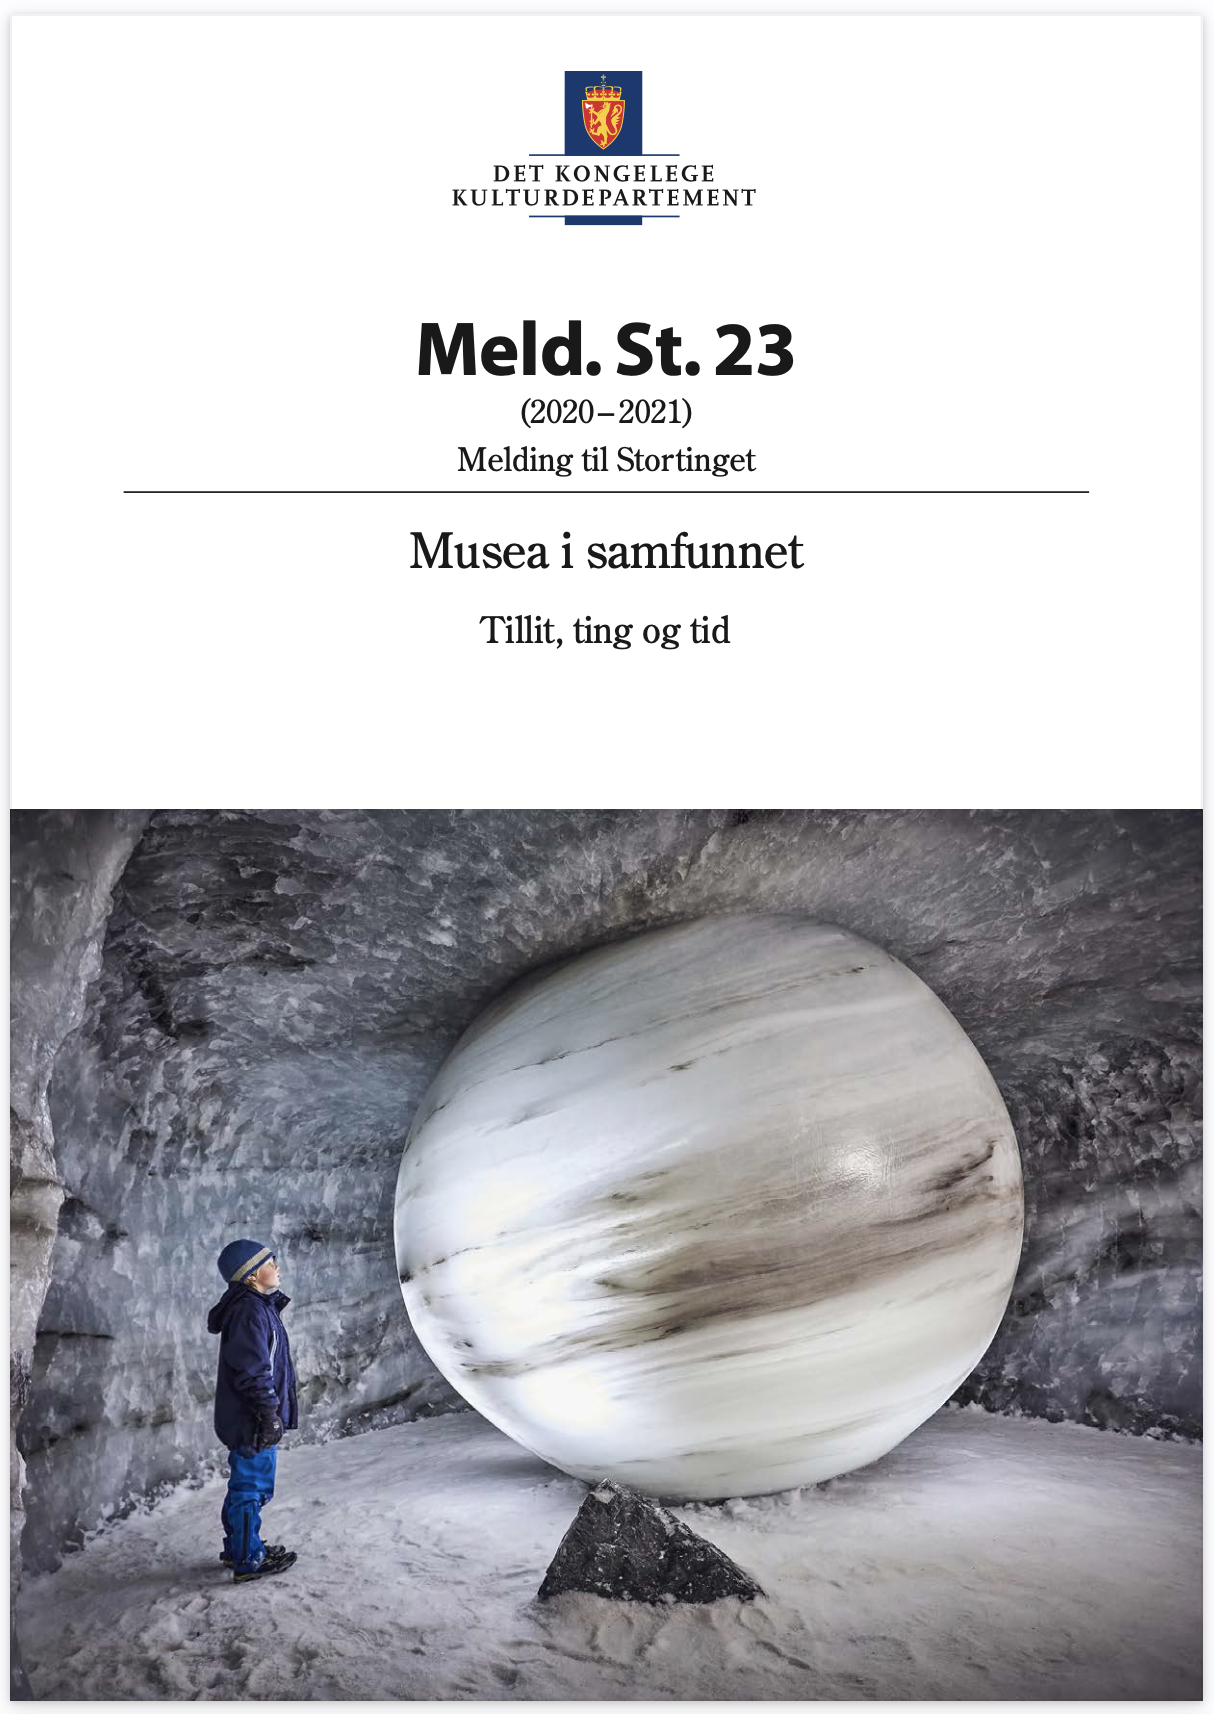
\includegraphics[width=8cm]{pictures/Introduction/stortingsmelding_hoykant.png}
\caption{The recommendation letter report Meld.St.23 \emph{“Museums in the society - trust, things and time"}} {\autocite[p. 1]{melding23}}
\end{figure}

There is a saying among historians that \emph{"the past teaches us about the present"}. History is a subject that is extra rich in perspectives, explanations, and ideas about how people have lived, thought, and acted. It positions us to see patterns that might otherwise be invisible in the present – thus providing a crucial perspective for understanding and solving current and future problems \autocite{UW_website}. Being a knowledge institution, museums have the power to both define and showcase relevant historical events as a perspective to inform present societal issues and debates. 

% Klimahistorie: eget avsnitt?

% Skiftet til museene handler ikke bare om å fornye seg, altså appellere til en bredere målgruppe, men det handler om å "henge med i tiden", og klare å forankre dagsaktuelle debatter/ samtaler med et faglig, vitenskapelig korrekt, blikk.

% Motivation: 

\section{Research Question/ Framing}
The aim of this study is to gain insight to try answer how one can design interactive meaningful experiences in a museum space that addresses sustainability. To understand this, several installations have been analysed as a way to objectify \emph{meaningfulness} as a quality that you can design for. In the HCI community, meaningfulness is recognised as a quality in made products or artefacts that not only make people more efficient and effective, but through use in activities, relationships, routines, and rituals, become meaningful \autocite{zimmerman_designing_2009}. This thesis fills a gap in the literature where the term is explored through a museum context for experience designers, trying to objectify meaningfulness as an interactive quality that support dialogic behaviour between visitors and installations in museums. Special attention has been given to museums that aim to encourage social action, like climate consciousness or climate action as examples of meaningful behaviour museums addressing contemporary discourses want to encourage.

This thesis aim to answer how one can design meaningful interactive experiences in a museum space that addresses sustainability. This is attempted through objectifying meaningfulness as a quality that you can design for in a museum, by identifying and analysing dialogic relations between visitor and installation.

In my attempt to answer how one can design meaningful interactive experiences in a museum space that addresses sustainability, I have composed concepts from three theoretical approaches to place-centred design to make my own theoretical framework to better understand interactive artefacts dialogic qualities and museum experience design. This attempts to answer how museum spaces can look at their respective installations and judge whether or not they stimulate the visitor to dialogue. The hypothesis is that there lies value for the museum to judge whether or not their installations promote dialogue.

\section{Scientific contribution}
The thesis investigates how interactivity can support visitors meaning-making in a museum space. The hypothesis is that an interactive installation or experience have the potential to reinforce the message conveyed in a manner that give rise to thought-provoking or significant reflections that last long after the museum visit. Something which also encompass the power to deliberately stimulate visitors lifestyle choices or actions after the museum visit, in compliance with the museums agenda and vision. 


\section{Chapter overview}
The thesis is divided into three parts; Introduction, Design Process, and Review/ Evaluation. The (report) structure reflects the methodological nature of doing Research through Design, where the Design Process is evidence of the practical activities shaping the thesis project. If not referenced otherwise, all pictures in this thesis come from a shared photo library the research buddies and I have built up and accumulated during fieldwork. The same goes for illustrations. If not referenced else-wise, they are illustrated by me.

\subsubsection{Chapter 2: Modern museums and sustainability}
Chapter 2 is a focused selection of terminology and concepts attained from the literature review that has been conducted throughout/during the thesis project. It is structured in the hope that designers interested in the topic can adopt the concepts as a vocabulary and mean of understanding some of what goes on in the museum world. The literature review has nonetheless been crucial for the thesis evolution. On the one hand, it has influenced the research framing and interest, shaped and refined the research question, and leveraged the vocabulary when documenting/ recounting an exhibition- and installation experience. While on the other hand, it has influenced the convergent and divergent thought process when going in and out/back-and-forth of practical and theoretical work, the designer role, and the researcher role.

\subsubsection{Chapter 3: Three approaches to place-centred design }
Chapter 3 is a continuation of the literature review. Where Chapter 2 indirectly affect the thesis evolution, Chapter 3 present three theoretical approaches that have formatively guided e.g. data-gathering guides during fieldwork, both for observations, interviews and analytical critique.

\subsubsection{Chapter 4: A new way of designing for meaningfulness?}
In Chapter 4, we build upon and borrow concepts from the three theoretical approaches presented in Chapter 3, in the making of a new theoretical framework as a proposal of a new way of designing for meaningfulness.

\subsubsection{Chapter 5: Methodology}
In Chapter 5 you can read on the methodological approach to Research through Design adopted through this thesis.  

\subsubsection{Chapter 6: Design Process}
In Chapter 5 you can read on the methodological approach to Research through Design adopted through this thesis.  


\subsubsection{Chapter 7: Analysis}
\subsubsection{Chapter 8: Discussion}
\subsubsection{Chapter 9: Conclusion}



\chapter{\ding{167} Modern museums and sustainability}

This chapter gives an introduction to literature from the museum field, starting with the ongoing transitional shift to a \emph{new} museology. The chapter will then introduce concepts and terms from exhibition and dissemination practise to extend the vocabulary for talking about museum subjects and roles. Then we will progress into sustainability as a topic representative of a contemporary discourse being addressed in a museum. The chapter is then rounded off with literature on the application and use of technology and interactive installations in "modern museums".

\section{The new museology}
% In this section we address the institutional shift and need in museology to challenge traditional museum practise.
In 1989, Peter Vergo coins the term \emph{the new museology} in a book bearing the same name. Museology is the study of museums, their history and underlying philosophy, and the various ways in which they have, during the passing of time, been established and developed \autocite[p.1]{vergo_museology_1989}. Vergo argue how beyond the physical material like handouts or information panels, there is a subtext comprising diverse and often contradictory strands woven from the intellectual, political or educational preconceptions from the museum stakeholders, e.g. the museum director, the curator, the scholar or the designer \autocite[p.3]{vergo_museology_1989}. Rather than 'old' considerations like administrative tasks, conservation techniques, financial well-being, or, success or neglect in the eyes of the public, the subject matter that should be more questioned or discussed should be more concerned with the museums \emph{purpose} rather than museum \emph{methods} \autocite[p.3]{vergo_museology_1989}. Vergo would therefore define the \emph{new} museology simply as a state of widespread dissatisfaction with the \emph{old} museology considerations. "Unless a radical re-examination of the role of museums within society takes place", Vergo declares that museums in this country (referring to the UK), and possibly elsewhere, may likewise find themselves dubbed 'living fossils' \autocite[p.4]{vergo_museology_1989}.

As Vergo would have it, \emph{"the museum world has undergone radical change since the 1970s. Political and economic pressures have forced its professionals to shift their attention from their collections towards visitors. Whereas in the past the museum tended to be exclusive and elitist, signs of a progressive opening-up and greater accessibility have appeared. A climate of increasing reflexivity within the profession is identified as a ‘new museology’."} \autocite[p. 84]{ross_interpreting_2015}.

\par
Jobbe litt med overgangen!: much literature have been written on the transition from old to new museology, such as (x, x, x). And then 'new' museology as part of the modernization of museums.
"One of the key terms today is learning in formal and informal contexts. Museums, too, are redefining their mission; instead of a focus on collecting and classifying, the emphasis is now on exhibition design and the museum as a place for communication and learning. The museum has thus become, perhaps more clearly than ever before, a place for education and learning, dialogue and debate (Hein 1998; Hooper-Greenhill 1994; Roberts 1997)." \autocite[]{insulander selander design for learning in museum context}


\subsubsection{Museum experience design}
Recent literature in the HCI field concerned with museums agrees that the museum world is rapidly changing from being collection-centred to being community-centred and for the public \autocite[p. 1]{vermeeren_museum_2018}. "Apart from broadening access to collections through, e.g., digitisation initiatives, new ways of involving the public more meaningfully and at various levels have emerged. Experiences inside museums have become more engaging, by extending the experience beyond the physical visit, or by involving the public in various forms of crowd-sourced stewardship of collections." \autocite[p. 1]{vermeeren_museum_2018}. In the book \emph{Museum Experience Design: Crowds, Ecosystems and Novel technologies} \autocite{vermeeren_museum_2018} present four key themes relevant for designers concerned with experience design in museums: 
\begin{itemize}
    \item Engaging the public,
    \item Cultivating diverse audiences,
    \item Availing ourselves of the benefits of digital technology,
    \item and, Leveraging museums’ roles as players in larger economic and cultural ecosystems.
\end{itemize}

 "Too often we (the museum) prioritize our mandate to hold and protect our collections and stop short of making them relevant to today’s audiences, real or potential. Too often we are zoomed way too far in on our objects, and lose sight of what people less invested might know, think, or want from us" \autocite[p. 1]{vermeeren_museum_2018}. In light of this, \autocite{vermeeren_vincent_2018} case on \emph{Becoming Vincent} is instructive where it among the findings is implied how "the importance of and attention to content is related to the increasing value associated with craftsmanship, in the belief that this will provide a real, genuine, and authentic experience" \autocite[p. 298]{vermeeren_vincent_2018}. "When we pull our focus back from the individual museum and its obsession with its objects, we find a larger community outside that is largely indifferent to our obsessions, and needs a story, even a superstar, to motivate their interest" \autocite[p. 1]{vermeeren_museum_2018}. "This is why storytelling can help turn any experience into a memorable and meaningful experience, by unlocking values that would otherwise be not so immediately recognizable by the listeners" \autocite[p. 299]{vermeeren_vincent_2018}.
 Then, "a struggle emerges between the museum’s role as protector of authentic objects and the “facts” around them and its role as a site of experiences—preferably extraordinary ones, because if not, why bother? "\autocite[p. 1]{vermeeren_museum_2018}. "So, while digital apps take us on mobile adventures and open up trails of wonder for some, the vast majority of our visitors still default to analog first and foremost. The more we can design for blended environments that mix the virtues of analog and digital affordances in mutually reinforcing ways to foster a context for meaningful engagement with museum objects, the better off we’ll be" \autocite[p. 1]{vermeeren_museum_2018}.


\section{Exhibition and dissemination practise}
In this section I will present terms and concepts to explain what I mean when I talk about exhibition and dissemination practise. This lays the foundation for the vocabulary which I have adopted throughout the literature review, and brought with me into the thesis project. 
% Comment more about how this section functions as both a literature review and as a practical vocabulary for "things to look for" .

\begin{figure}[H]
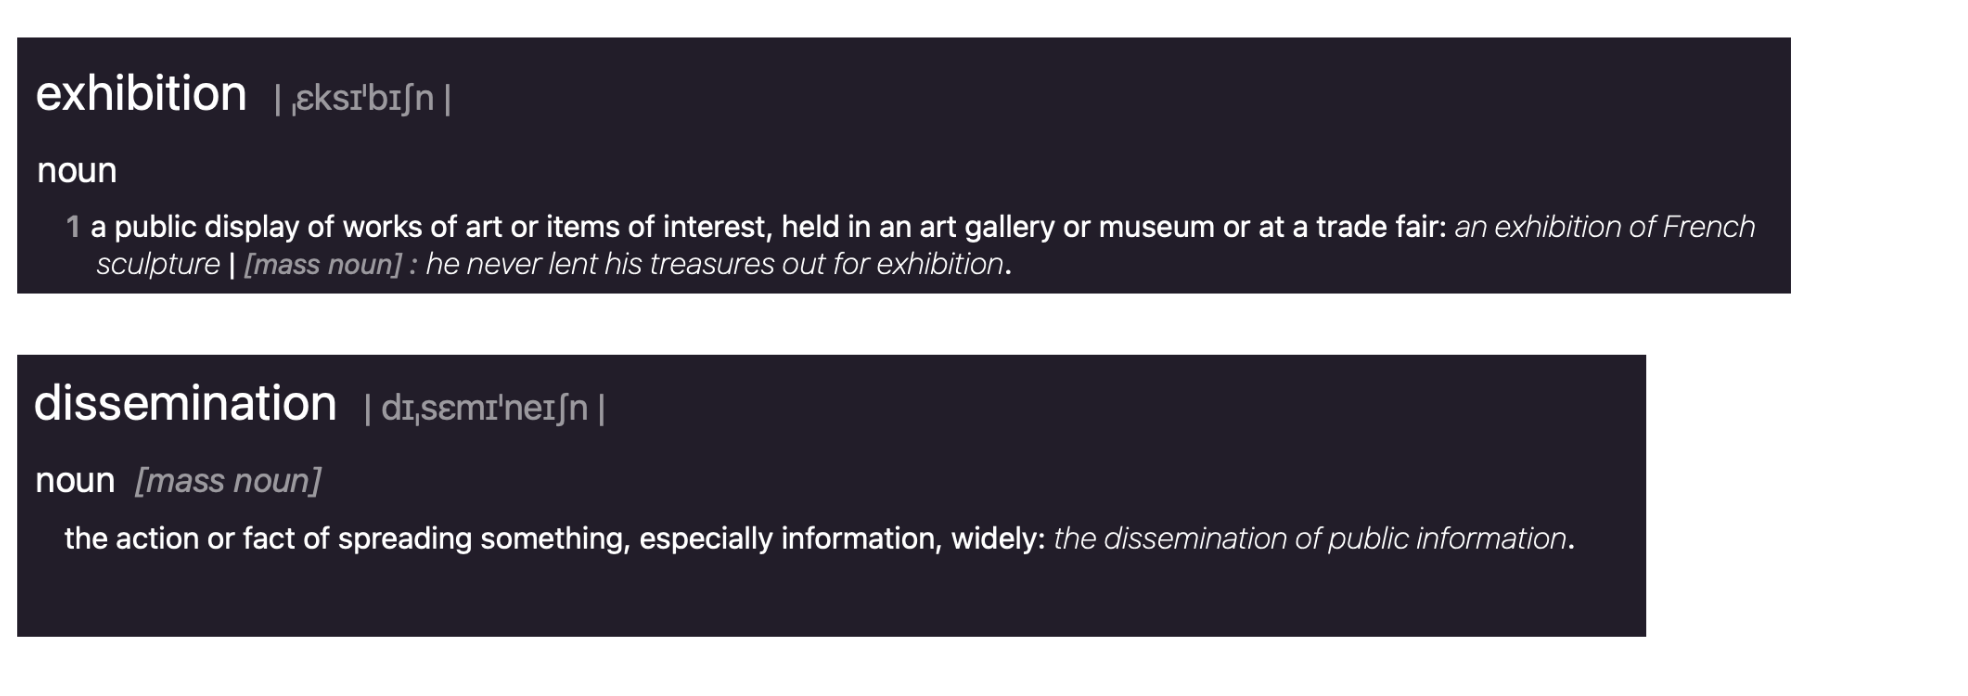
\includegraphics[width=14cm]{pictures/background/exh_diss.png}
\caption{Definitions from the Oxford dictionary of English (UK).}
\centering
\end{figure}

\subsection{Museum discourse and cultural moralism} 
% and look for power structures/ imbalances (cultural moralism or imperialism) in terms of addressing sustainability in museums
In this section one of the major influences from critical humanities literature is presented, which vocabulary have helped to better “read”, describe and understand a museum, exhibition or a specific installation. Mieke Bal is a dutch cultural theorist, video artist and Professor in Literary Theory at the University of Amsterdam, with academic interest and background in humanities, media and culture studies. From her writings on cultural analysis and discourses in the museum, she proposes a humanistic perspective on what differentiates the “new” from the “old” museology, where she presents the museum as a discourse and the exhibition as an utterance within that discourse. By bringing this discursive perspective to the museum, it deprives the museal practise of its innocence, and provides it with the accountability it and its users are entitled to \autocite[p. 214]{Thi_book}. Part of her argument and critique is that politics come straight out of, or more precisely are bound up with, the museal discourse \autocite[p. 214]{Thi_book}, and proposes a threefold direction to museology researchers. First she suggest to systematically analyse the narrative-rhetorical structure of the specific museum, in order to refine the categories and deepen insight into their effects. Secondly she suggest to look at the connection between the museal discourse and the institutions foundation and history, and thirdly she see the need to do self-critical analysis of the museal discourse as a consequence of the nature of discourse. % kanskje nevne at hun særlig har studert: cultural moralism and cultural imperialism i museer som tidligere har disseminert kolonialisering som et tema for globalisering i museer.. 

With my background and scope of thesis it is both irrelevant and I am by no means capable to do a discursive analysis the way Mieke Bal proposes. I do however find aspects of Bal’s discursive perspective relevant, like her proposal of how one can do a narrative-rhetorical systematic analysis of a specific museum. She provides a set of new terms and vocabulary so that I better can “read”, describe, understand and do research on a specific museum and/ or specific installation. I find this perspective along with the extended vocabulary it provides useful so that I better can identify meaningful relations between user activity at installations/ artefacts and the museum experience.

\begin{figure}[H]
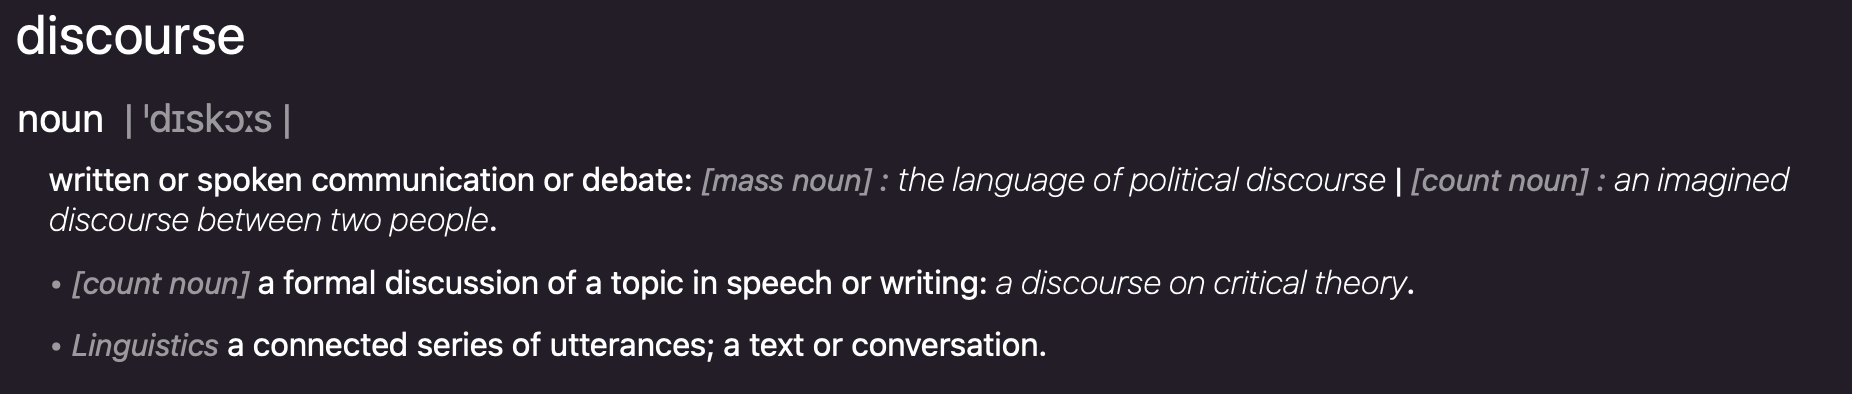
\includegraphics[width=12.5cm]{pictures/background/discourse.png}
\caption{Definition of Discourse from the Oxford dictionary of English (UK).}
\centering
\end{figure}

The museum is an attractive object of study because it requires interdisciplinary analysis; it has the debate on aesthetics at its core, and it is essentially a social institution \autocite[p. 202]{Thi_book}. % Cultural moralism is a concept described as (...xxx...), fronted by Mieke bal.....::
Mieke Bal account for and describe the issue of cultural imperialism in museums, exemplifying case studies related to natural history types of museums that conserves and display ethnic objects and artefacts representing cultures and cultural properties from the past. The ethnographic museum is clearly the most obviously politically charged institution, and it poses the immediate problem of cultural property and collective ownership \autocite[p. 202]{Thi_book}. It raises the question if former colonists are entitled to hold onto objects taken by their ancestors from former colonies, or should they give these back to the country of origin the ancestors of whose inhabitants were their original owners? % Vergo also say something about this, the "problem" of museums placing objects to/ and from cultures. Often to display power. 

I think this (critical and) introspective perspective is necessary to have in a museum context or space addressing sustainability, because the intention of making a meaningful interactive experience is to strengthen the message conveyed by the museum. Both the designer and especially the museum need to be aware of and able to answer to the moral and ethical questions raised in terms of what the message they convey, actually conveys. And that the act of strengthening that message actually send people out of the museum with reflections and thoughts that hopefully leads to social action (climate action, consciousness). % Do the museum "have the balls" to stand up for and answer to the kind of actions they actually promote?

\subsection{Artefacts, artworks and installations}
The very act of collecting has a political, ideological or aesthetic dimension which cannot be overlooked, and Vergo questions; "what makes certain objects, rather than others 'worth' preserving? \autocite[p. 2]{vergo_museology_1989}. "The original intention behind the establishment of museums, was that they should remove artefacts from their current context of ownership and use, (...), and insert them into a new environment which would provide them with a different meaning" \autocite[p. 6]{vergo_museology_1989}. "The essential feature of museums - and what differentiates them from the many extensive private collections which preceded them - was, at first, that the meanings which were attributed to the artefacts were held to be arbitrary; and, second, that the collections should be accessible to at least a portion of the public, who where expected to obtain some form of educational benefit from the experience" \autocite[p. 6]{vergo_museology_1989}.

The heritage museum conserves and exhibits artefacts, while the art museum, works of art. It seems obvious what differs the artefact vs the artwork; yet they differ in regard as to what they represent. Both the artefact and the artwork is charged with cultural meaning. It tells us about a larger cultural situation, e.g. aesthetic conceptions or world views, conceptions of representations or the social relevance of art. However, these meanings is only yielded if we are able to “read” it, or is put in some context that illuminates the cultural meaning \autocite[p. 206]{Thi_book}.

The term artefact suggests a man made object charged with cultural meaning which can, if studied carefully, offer us information on the society in which it has been created \autocite[p. 205]{Thi_book}. The difference between the artefact according to the above definition and the common idea of art is that the former takes for granted what the other represses: the possibility of cultural difference. Instead, artworks are viewed as standing for an aesthetic, and is therefore considered metaphors, transferring their specific aesthetic to the one current sufficient to make the work “readable” as art, regardless of what it could tell us about the culture it comes from \autocite[p. 206]{Thi_book}. While the ethnic artefact, in contrast, is first and foremost considered to be a representative of the larger context of the culture it comes from \autocite[p. 206]{Thi_book}. Hence, it is not a metaphor but synecdoche. Synecdoche is the figure of rhetoric where an element, a small part, stands for the whole simply by virtue of its being a part of that whole \autocite[p. 206]{Thi_book}. Thus the artefact is only readable as culture, no matter what aesthetic qualities it may also have.


\subsection{The curatorial function}
% Kanskje introdusere med noe sånn: Fra boken (thinking about exhibitions), kapittel 1 skriver (Carmen?) om kuratorens rolle i museet. 
The curator are, above all, the institutionally recognised experts of the art-world establishment, whether they operate inside an institution or independently. More than art critics or gallery dealers, they establish the meaning and status of contemporary art through its acquisition, exhibition, and interpretation \autocite[p. 22]{Thi_book}. To a greater extent than other art-world professionals, curators additionally depend on an established infrastructure to support their efforts. This infrastructure includes institutionalised networks, such as those provided by museums, galleries, or alternative spaces; financial sponsors, whether public, private or corporate, and teams of technical or professional experts \autocite[p. 22]{Thi_book}. Curators are the sanctioned intermediaries of these institutional and professional networks on the one hand, and; artists and audiences on the other. The curatorial function is, this, inherently restricted by the interests of the larger or more powerful groups and constituencies in the museum \autocite[p. 22]{Thi_book}.

By selecting, framing and interpreting peripheral art in exhibitions and exhibition catalogues, for instance, art curators can claim to be shaping a more democratic space where specific cultural groups can recognise themselves \autocite[p. 23]{Thi_book}. As the debates of recent years have shown, “identity” is not an “essence” that can be translated into a particular set of conceptual or visual traits. It is, rather a negotiated construct that results from the multiple positions of the subject vis-a-vis the social, cultural and political conditions which contains it. How then, can exhibitions or collections attempt to represent the social, cultural and political complexities of groups without reducing their subjects to essentialist stereotypes? \autocite[p. 23]{Thi_book}.

This situation places the cultural broker at the very core of a contradiction: on one hand, she can be credited for helping to tear down artworld hierarchies, seemingly democratizing the space for cultural action; on the other hand, in a market scenario where “identity” can only be a reductive construct, the framing and packaging of images of the collective self can only result in a highly delusionary enterprise \autocite[p. 23-24]{Thi_book}. The tensions of this contradiction confront art curators with a dilemma; where should they position themselves vis-a-vis the identities of the groups they claim to respect? \autocite[p. 24]{Thi_book}.

\subsection{Dialogical engagement}
"Museums started off as institutions focusing on collecting and preserving objects, open for the public to come and watch. The primary purpose for visitors to come to the museum was to see the original objects. A first notable shift saw the museums move from a collection focus to a visitor focus and from a mission for objects preservation and access provision to a mission of offering meaningful engagements with the collection and rewarding learning experiences for their public. The concept of ‘museum experience’ is the pinnacle of this historical shift, as it implies a focus on the visitor and connections between visitor and objects rather than a focus on collections. In the course of time, new types of museum experiences gradually emerged. The degree of sophistication and immersion increased exponentially when experiences started to be enhanced by the integration of interactive and digital media. In many science and technology museums, for example, visitor engagement and participation are uplifted through the use of new media (e.g. video games, interactive installations and other forms of edutainment) to encourage visitors to engage with the content on exhibit, to experiment with the techniques on show and to appropriate the visiting experience by making it meaningful and memorable. This trend is being adopted also by art museums, where it is by definition more difficult to let visitors experiment with the collections." \autocite[p. 3]{vermeeren_museum_2018}.

\begin{figure}[H]
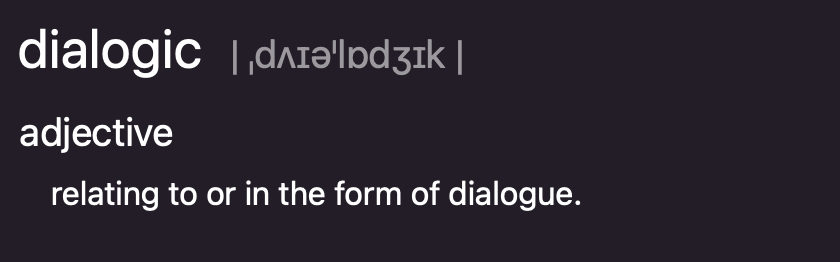
\includegraphics[width=6cm]{pictures/background/dialogic.png}
\caption{'Dialogic' defined in the Oxford dictionary of English (UK).}
\centering
\end{figure}

\subsection{Museology and the Anthropocene}
In a call for publication and participation to the conference "The future of tradition in museology" organized by ICOFOM in Kyoto 2019, the same institutional change and questions concerning the future of museology that we just have read through the eyes of \autocite{ross_interpreting_2015}, \autocite{vergo_museology_1989} and \autocite{vermeeren_museum_2018}, is addressed. They present five directions to be considered worthy of further research, whereas two of them stand out in term of this thesis's research interest. \autocite[p. 4]{icofom_kyoto_2019}:

\begin{itemize}
    \item \textbf{Museological tradition vs global development and new technologies:} What role does museology play and what position does it take in relation to the rapid changes that are taking place? (...), e.g. will cyberspace out rule other spaces and materialities – (...), considering the return to extreme political positions and the “war” of information and knowledge?
    \item \textbf{Museology and the Anthropocene:} How can museology reduce the disastrous effect man has on our planet earth and our living conditions? How can museology help to bridge the gap between mind and matter – the gap that is the reason for the state of mankind right now – the belief that man is superior to nature and all other creatures? (...) So what impact should this insight bring to our dealing with museums, objects and collections, with a sustainable future in mind?
\end{itemize}

\begin{figure}[H]
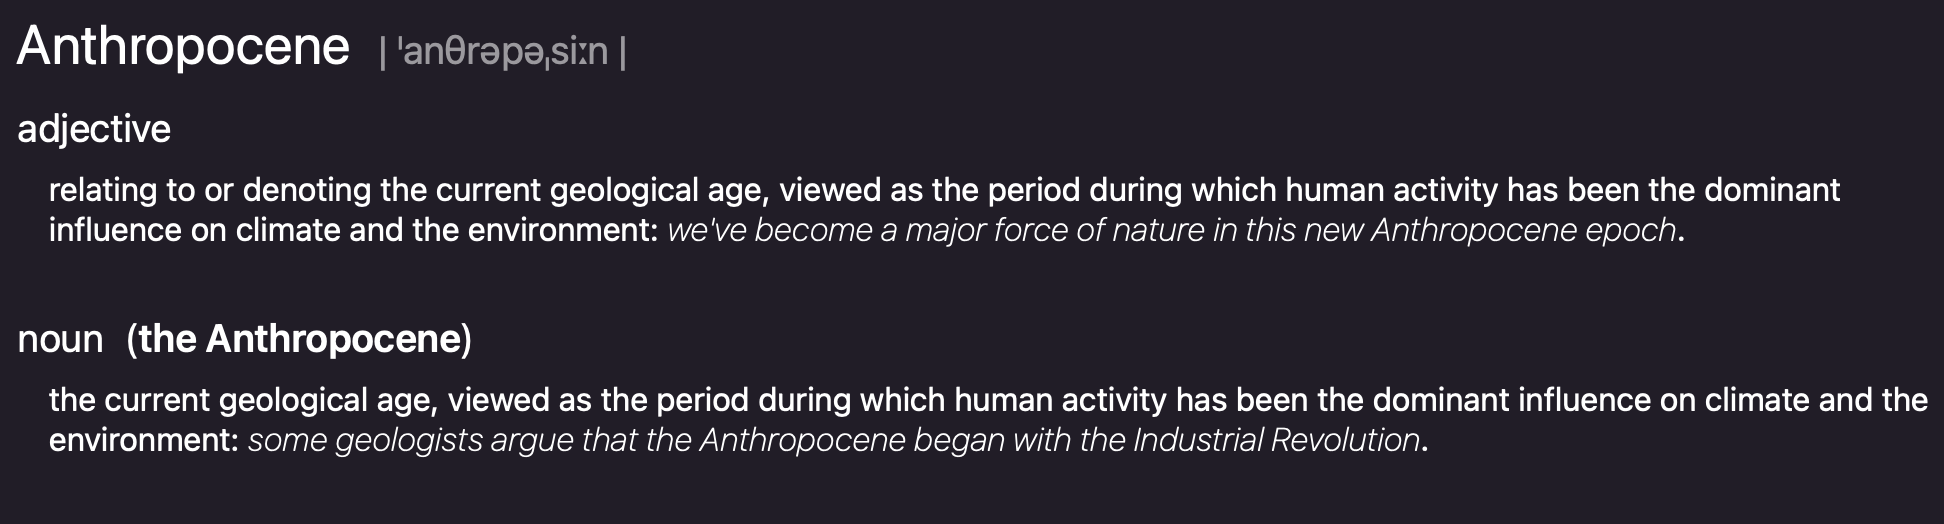
\includegraphics[width=12.5cm]{pictures/background/anthropocene.png}
\caption{Anthropocene definition from the Oxford dictionary of English (UK).}
\centering
\end{figure}

\section{Museums communicating the science of climate change}

"Social research underlines how the mass media frames and presents environmental change and risk in ways that become contested cultural constructs embedded in deep ideological structures" \autocite[p. 1]{salazar_mediations_2011}.\emph{ While significant attention has concentrated on the mass media, less consideration has been given to examining the role of museums and science centres in communicating the science of climate change} \autocite[p. 1]{salazar_mediations_2011}. In the article "The mediations of climate change: museums as citizens media" \autocite{salazar_mediations_2011} looks at museums as cultural brokers around the public understandings of climate change. By engaging with recent conceptualisations around citizens and public media practises, Salazar proposes mechanisms through which the museum sector can act as change-agents in fostering a new form of public pedagogy that incorporates differing civic epistemologies around climate change education and action" \autocite[p. 1]{salazar_mediations_2011}.

\begin{figure}[h]
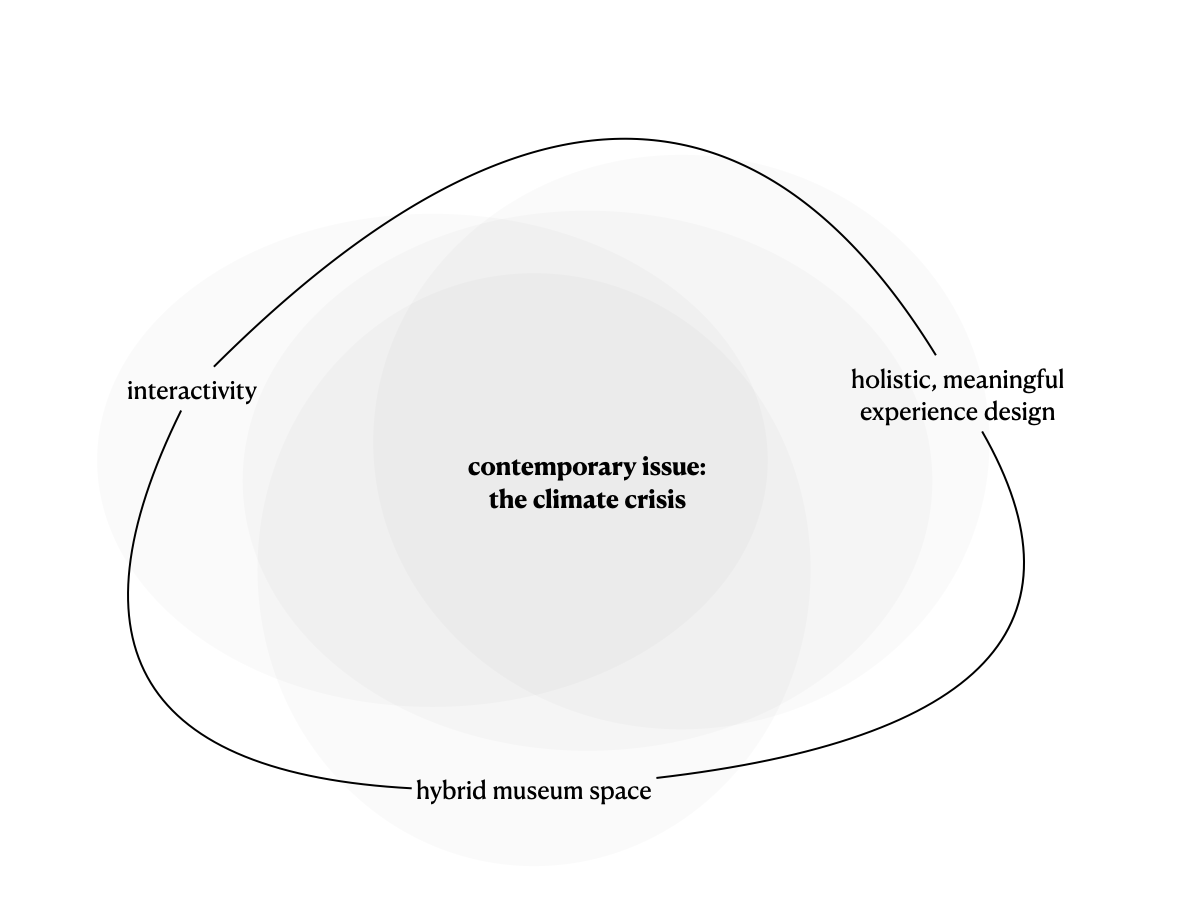
\includegraphics[width=10cm]{pictures/problem_sphere.png}
\caption{My representation of sustainability issues in museums}
\centering
\end{figure}

% https://www.youtube.com/watch?v=GOhfxHHhqpg: Art installation for World Oceans Day at the California Academy of Sciences by futurists Wallace J. Their installation \emph{Plastic Century} is an interactive installation created for the California Academy of Sciences that explores the relationship between plastic, people, and the environment over the 100 years since the birth of Jacques Cousteau.

In a commentary by Richard J. Hebda, they look into the Royal British Columbia Museum (RBCM)’s voyage into the issue of climate change as an example of how museums can play a central role in addressing contemporary issues. Traditionally, museums have been a window to the past, "a place where the past lives" \autocite[p. 1]{hebda_article}. A lot of the issues and societal attitudes that are addressed in the commentary are still relevant today. Traditionally, human history and natural history has been seen as two solitudes that have been exhibited separately. A key appeal for the RBCM, a typical natural history museum to do a climate change exhibit, was to pursue the opportunity to link and integrate the two solitudes in a compelling and relevant manner \autocite[p. 2]{hebda_article}. They justify that the combining of the two is necessary because the exact same challenge is also central in the sustainability debate, at the core of the problem facing society today \autocite[p.2]{hebda_article}. In 2007 when the RBCM decided to make the climate change exhibition, the question of climate change was still a controversial issue \autocite[p.2]{hebda_article}. Addressing the increasing evidence and knowledge in terms of climate change and how it affects and is affected by humans, nearly all reputable scientists felt that change was under way and action was needed \autocite[p.2]{hebda_article}. The political and public atmosphere was foggy, as people did not know whom to believe, what information was science-based rather than rhetoric, and where real uncertainty lay \autocite[p.2]{hebda_article}. The RBCM saw a clear opportunity to dispel the fog and to enlighten their audiences \autocite[p.2]{hebda_article}.

\subsubsection{Changing Climate, Changing Attitude?}

"Many science museums and science centers now recognize their potential to arouse young peoples’ interest and awareness, and are starting to engage them in the climate change debate (e.g. Science Museum London, Australian Museum, Aquarium San Diego, American Museum of Natural History)" \autocite[p. 95]{gorr_changing_2014}. "Whereas some studies show evidence that museum and science center experiences may result in attitude change (Smithsonian Institution 2011; Spock 2000), there is evidence from a range of environmental-related exhibitions that initial changes in attitude and understanding fade after a couple of weeks because museum visitors tend to seek confirmation of their pre-existing attitudes and cling to erroneous beliefs (Adelman, Falk, and James 2000; Cakir 2008; Dierking et al. 2004)" \autocite[p. 95]{gorr_changing_2014}. "Some examples have even illustrated that attempts to increase people’s understanding of climate change enhanced skepticism and resulted in visitors’ total rejection of the issue (Jones 2009; Webster 2010)" \autocite[p. 96]{gorr_changing_2014}.

"Aiming to examine attitude changes in young people, the described study drew on general findings about attitude from social sciences and psychology. A closer look at the theory reveals that attitude is a highly complex and ambivalent term; for instance, a person may want to express both positive and negative attitudes toward the same object (Wood 2000). Whether an experience leads to longer lasting attitude change depends on numerous aspects such as motivation and attention (Petty and Cacioppo 1986). Motivation is mostly dependent on clarity and on the personal relevance of a message (Petty and Cacioppo 1979; Salazar 2011), or it may result from emotions, such as empathy and enjoyment (Roberts 1993)." \autocite[p. 96]{gorr_changing_2014}.



\section{Design as Meaning Making}

\autocite{kazmierczak_meaningmaking_2003} approaches design as an interface for meaning making, or simply the design of meaning. She see "meaning" as standing for a thought induced in the receiver, originated by contact with a design. According to her, design can be simple or complex in their material and conceptual structure but, as wholes, they are interfaces for meaning making \autocite[p. 47]{kazmierczak_meaningmaking_2003}. Borrowing from literature on cognitive semiotics, she proposes a model for design which relates physical form to cognition and comprehension rather than appearance and aesthetic. According to \autocite{kazmierczak_meaningmaking_2003}, there are two reasons why cognitive semiotics offers potentially good results; \emph{"First, it is focused on bridging the gap between form and meaning making or comprehension. Thus, its method of inquiry makes it well equipped for a discussion of symbolic-cognitive human phenomena such as communication. Second, it is compatible with the concerns of design regarding the construction of communications"} \autocite[p. 47]{kazmierczak_meaningmaking_2003}. 

\begin{figure}[H]
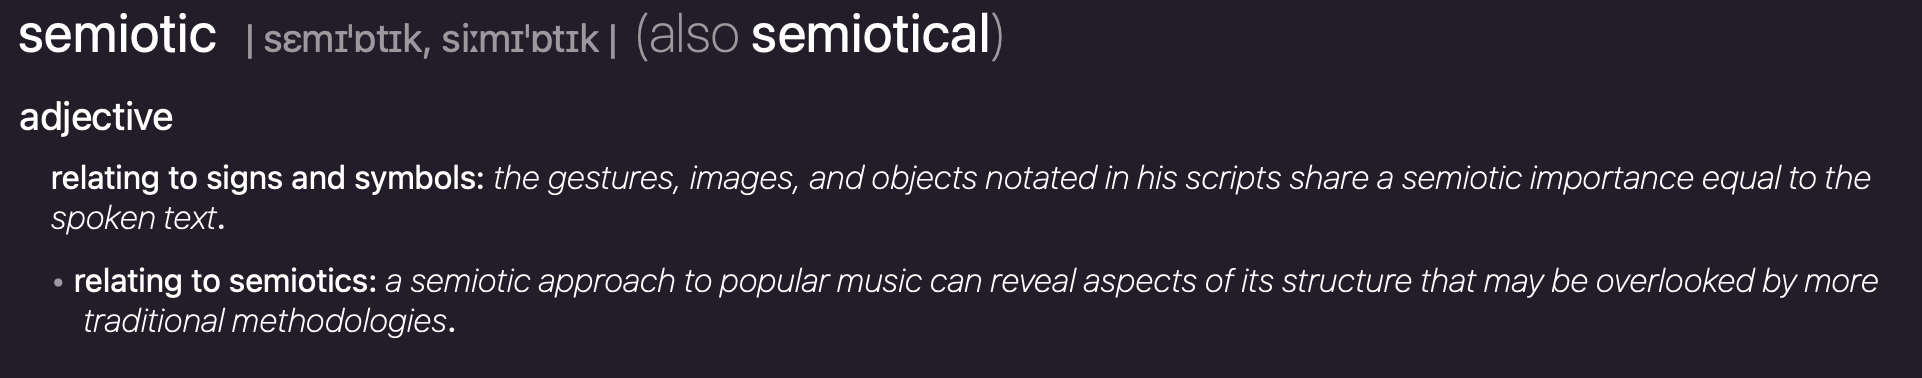
\includegraphics[width=12.5cm]{pictures/background/semiotic.png}
\caption{Definition of Semiotic from the Oxford dictionary of English (UK).}
\centering
\end{figure}

Textual and written components are essential in any museum; 

I would argue that bringing cognitive semiotics (relating to signs and symbols) can be a useful perspective when working in/ designing for museums. It enables the designer to see the museum agenda and curatorial function up against the designed object, and when working with interactivity to emphasise dialogic qualities it should be useful to have the means to see, discuss and question the semiotic aspects of the designed object..... Museums that not only are 

\begin{figure}[H]
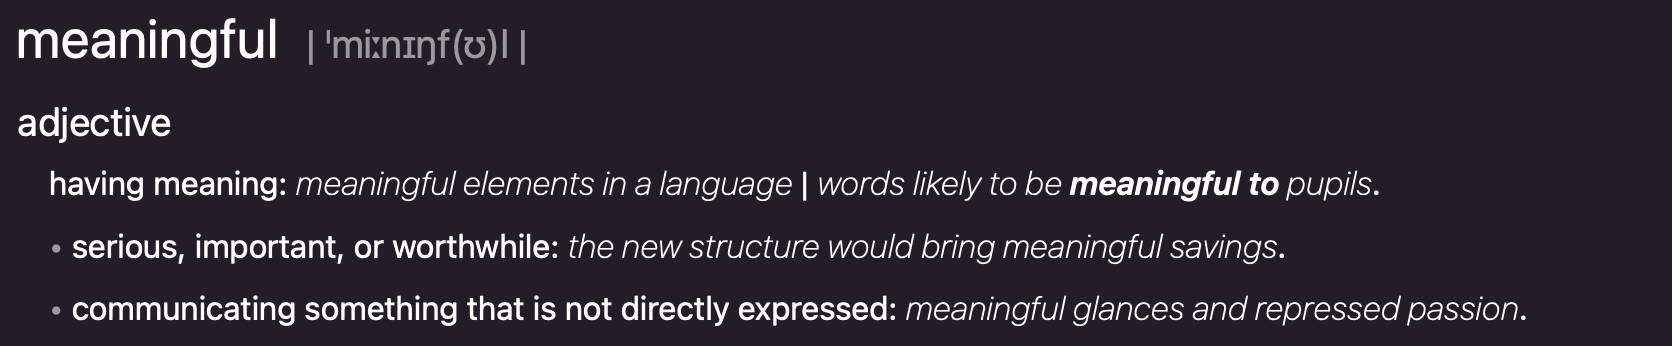
\includegraphics[width=12.5cm]{pictures/background/meaningful.png}
\caption{Definition of Meaningful from the Oxford dictionary of English (UK).}
\centering
\end{figure}


\begin{comment}

Hvordar forstår jeg bærekraft, og hvorfor mener jeg det er viktig?
Hvordan snakker andre om det, og hva må jeg få sagt til leseren om bærekraft?
Hvordan “angriper” jeg bærekraft temaet inn i denne oppgaven? 

\begin{figure}[h]
\includegraphics[width=8cm]{pictures/museumintersections.pdf}
\caption{Can the intersection between museal exposition, the museums exposition of arguments and their exposure of cultural artefact provide data or finds on power structures/ tensions/ imbalance in museums? Especially in terms of sustainability?}
\centering
\end{figure}

\end{comment}

\chapter{\ding{167} Three approaches to place-centred design}
This chapter is a continuation of the literature review, however, three theoretical approaches to place-centred design is presented; Hybrid Place, Place as a dialogue, and, Sense-making. These approaches have all directly guided fieldwork and analysis-oriented efforts, and as you will come to see in Chapter 4, we build upon and borrow concepts from all three approaches to build a theoretical framework that can help both identify and analyse dialogical relations in a museum space.

\subsubsection{Technologically-enhanced physical spaces}
The perspective of “Ubiquitous Computing,” proposed in the early 1990s by Mark Weiser, is based on technological developments that make it possible to embed powerful computational elements and digital components into everyday objects, portable devices, and the built environment \autocite[p. 217]{ciolfi_space_2005}. This trend is inducing significant changes not only in the development and implementation of new technology but also, and more interestingly, in the relationship between interactive systems and their users \autocite[p. 217]{ciolfi_space_2005}. Design must now concern itself with the physical environments people experience in their daily lives. People will encounter technologically enhanced spaces and artefacts as they move through a variety of environments \autocite[p. 217]{ciolfi_space_2005}. These systems will change how physical spaces are used and shaped by people, where the systems can react and respond to their presence and actions. The activities of interacting with the space and its elements and interacting with the computer system will merge into each other \autocite[p. 217]{ciolfi_space_2005}.

The Interaction Design (IxD) field is currently enduring a shift in the understanding of the relationship between people and technologies, where HCI primarily has focused on a single user's traits and preferences, a one-to-one relationship with the computer system \autocite[p. 217]{ciolfi_space_2005}. As a result, interaction Design is now more than ever concerned with the social, emotional, and contextual factors influencing human interaction with a computer system \autocite[p. 217]{ciolfi_space_2005}. Context-aware systems are those that can sense features of the physical setting and feed a representation of this data into the system itself. The sensing devices can be located both around the physical environment and on the bodies of the inhabitants \autocite[p. 218]{ciolfi_space_2005}.

Ciolfi and Bannon's research aim to apply the concept of a place to a particular set of ubiquitous systems: technologically-enhanced physical spaces. With ubiquitous technologies becoming more reliable and widespread, we are now dealing with fully interactive physical spaces containing tangible elements acting as interfaces to access features of the digital domain. The way this is applied and understood in this thesis, the concept of place can assist interaction designers in understanding interaction dynamics in this context. This way, one can aim to propose practical design concepts: "where place goes beyond the vision of space just as a physical setting, a container, and includes many dimensions of human experience within an environment" \autocite[p. 221]{ciolfi_space_2005}.


% Illustration of Hybrid Place?
\break
\section{Hybrid Place}
This section presents the Hybrid Place approach. As the thesis unfolds, I will often refer to this approach as it is; either \emph{the Hybrid Place approach} or simply \emph{Hybrid Place}. This is a place-centered approach to how geographical notions of space and place can aid designers in creating meaningful interactions between end-users and technologically augmented physical spaces. This is aided through four dimensions, presented in section 3.1.2. The four dimensions have both a formative application for the design of the data-gathering guides, as evident in the Appendix, the Design Process (Chapter 6), and Chapter 4: A new way of designing for meaningfulness.

\subsection{Designing a hybrid place}
"Thanks to the development of ubiquitous and pervasive technologies, research focusing on the design of novel interactive artefacts has recently become more concerned with studying and understanding the spatial properties of the world" \autocite[p. 159]{hybridplace_ciolfi}. "Bringing technologies beyond the desktop and into the world requires an ever-increasing interest in the \emph{physical environment} where interaction occurs" \autocite[p. 159]{hybridplace_ciolfi}. "Designing the interaction between ubiquitous technologies and users involves both a re-conceptualization of the interface as an assembly of tangible physical elements (including furniture and everyday objects) and, importantly, an understanding of the relationship between users and the physical space that is augmented by the technology" \autocite[p. 159]{hybridplace_ciolfi}. Following the interest in the physical environment where interaction occurs, Ciolfi and Bannon discuss how geographical notions of space and place can aid designers in creating meaningful interactions between end-users and technologically augmented physical spaces. After reviewing literature discussing the use of spatial concepts and metaphors within the interaction design field, they present a conceptual framework to design technologically enhanced environments for museums and exhibitions. Their goal is to show how a place-centered approach can practically guide and support design, specifically within a setting that has seen many cases of technology introduction that have led to the visitors' distraction from the museum holdings instead of extending and supporting the museum experience \autocite[p. 159-160]{hybridplace_ciolfi}.


Ciolfi and Bannon (2007) are particularly interested in the experience of place. They strive to understand the ways people come to ascribe meanings to particular places and how certain places evoke complex webs of significance for people \autocite[p. 160]{hybridplace_ciolfi}. This is different from other similar research approaches that have attempted to use ideas from architecture and urban planning to inform the placement of interactive artefacts, e.g., \autocite{Cullen_book}, or noting how the environment affects people's movement and interaction, e.g., \autocite{Alexander_book}. Instead, they base their articulation of place on the work of the geographer \autocite{Tuan_book}. According to Tuan, it is only natural that a place is grounded in the physical, material reality of the world. And that experience is shaped through physical sensing, exploration, and habitation. Based on Tuan's conceptualizations, Ciolfi and Bannon propose an articulation of the concept of place that highlight the different dimensions as interconnected aspects of the individual experience, see Figure 3.1:

\begin{figure}[H]
\centering 
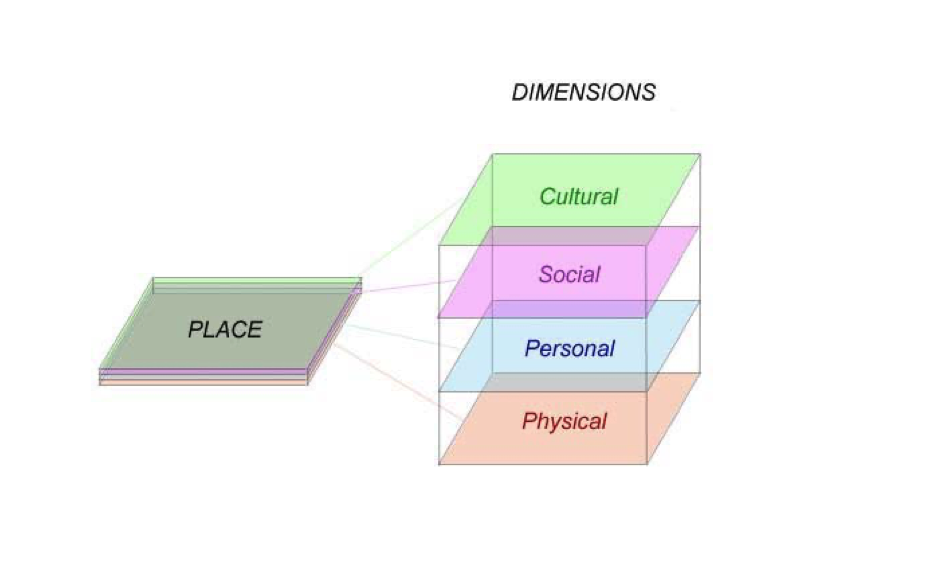
\includegraphics[width=12.5cm]{pictures/Theory/tuans_dimensions.png}
\caption{Tuan's conceptualization of place}
\autocite[p. 224]{ciolfi_space_2005}
\centering
\end{figure}

The articulation of the four dimensions of place can help interaction design in interactive spaces by bringing aspects of individual traits and preferences, social interaction, and cultural influences together with the physical features of the space \autocite[p. 163]{hybridplace_ciolfi}. "These dimensions do not exist \emph{a priori}, but emerge and become visible in practice and experience as they lead to and emerge through people's actions and activities in the museum space or with the installation" \autocite[p. 163]{hybridplace_ciolfi}. As Ciolfi and Bannon explain it, each dimension is present at any moment of one's experience of place, but the dynamic interconnections shape the experience itself among these dimensions. Each particular experience of the place is both individual and unique, although influenced by the presence of- and interaction with others. "Others" could be the other visitors in the museum or, e.g., a group of friends or family visiting together, as is expressed through the social dimension. In order to understand a place and its inhabitants, all four dimensions and their interplay have to be taken into account \autocite[p. 162]{hybridplace_ciolfi}.

Ciolfi and Bannon argue that a place-centered approach can practically guide and support museum experience design. I have found this approach helpful in the process of understanding how one can design interactive and meaningful museum experiences. It helps position and argues why and how the context, e.g., the surroundings and environmental qualities, influences the one-another impression of the museum and the exhibition, or a particular installation. The concept of the museum being a hybrid place can help to understand interaction dynamics in the museum context. In addition, it provides a vocabulary and a theoretical lens to talk about and understand a specific experience with e.g. an interactive installation. The level of abstraction on the four dimensions provides an opportunity to incorporate different types of museum experiences. This can be useful in the initial stages of a design process when getting to know a new museum context. It provides a holistic lens to help read the room and learn its dynamics concerning the discourse. I hypothesize that interactivity alone will not build a meaningful experience. Instead, a meaningful experience is rather a close interplay between the installations in the narrative path that the museum builds as the exhibition and a way to remember the place where the meaningful experience occurred. Then, over time, when months or years have passed, and the details of the experience are forgotten, what remains is the memory of something meaningful happening in that place; the museum. That is what makes you want to come back to the museum, possibly bringing friends and family so that they too can experience something meaningful.


\subsection{Four dimensions}
When it comes to designing a hybrid place, as researched by Ciolfi and Bannon (2007), the main contribution is the place-centered approach that provides the basis for discussing the place-related qualities in the museum of study. In Ciolfi and Bannon's case, they used the approach to highlight the limits of existing technologies and to propose the design of novel ones \autocite[p. 163]{hybridplace_ciolfi}. In contrast, I am interested in using the place-centered approach to highlight meaningful relations in the museum.

Ciolfi and Bannon conducted a case study \emph{the design of the interactive exhibition 'Re-Tracing the Past' at the Hunt Museum, Limerick}. The study shows how attention to place and its dimensions can inform design in quite concrete ways and help in overcoming the problems of current interactive museum installations \autocite[p. 178]{hybridplace_ciolfi}. Through the development of their conceptualization of 'place', involving people's lived experience of the physical space, based on \autocite{Tuan_book}'s work; they articulate four dimensions of place: physical, individual, social, and cultural \autocite[p. 178]{hybridplace_ciolfi}. Their evaluations demonstrate that the exhibition they designed supported visitors' engagement with museum artefacts, encouraged social interaction, discussion, and debate, and allowed for personal and unique contributions to the place \autocite[p. 178]{hybridplace_ciolfi}. Through the case study of 'Re-tracing the Past', they derived four dimensions where the consideration of the multiple dimensions of peoples experience allowed to pinpoint issues to be dealt with in the design phase \autocite[p. 178]{hybridplace_ciolfi}. These issues are as following:

\begin{itemize}
    \item How people appreciate the exhibit
    \item How people interact with eachother; and
    \item How people devise their own path through the exhibits and leave a trace of their presence in the space.
\end{itemize}

These "issues" are place-related considerations that can prove useful to take note of when designing to support or extend an experience. In the search as to how one can design for meaningful interactive experiences in a museum space, these considerations will let already existing dialogic patterns come to the surface. \autocite{hybridplace_ciolfi}'s four dimensions are made as one way to uncover what place-related patterns and behaviour already happens in the museum:

\begin{itemize}
  \item \emph{The physical/structural dimension:} Relating to materials, structures and environmental factors. The exhibition should be aesthetically pleasing pleasing in order to merge harmonically with the museum; it should should be a space that favours participation and active discovery; it should be welcoming and friendly; it should support group interactions as well as individual's, and be accessible by different age groups.
  \item \emph{The personal dimension.} Related to the feeling and emotions we associate to a place, to the memories related to or evoked by it, to the personal knowledge and background we invest the place with while making sense of it. The exhibition should not have a prescribed sequence of actions in order to allow visitors to configure their visit; the exhibition should encourage visitors to express their opinions, comments and reflections and, to some extent, to leave their own trace; the visitors should feel welcomed and at ease. 
  \item \emph{The social dimension.} Related to social interaction and communication within the place, to the sharing of resources and memories, to social co-ordination and ethics, etc. Social interaction among groups of visitors should be supported and favoured. Also, the museum Docents should be encouraged to take part to the exhibition together with visitors.
  \item \emph{The cultural dimension.} Related to the rules, conventions and cultural identity of a place and of its inhabitants. The exhibition should be a representation of the museum's culture and identity. It should also suggest to visitors that - although located within a museum - the conventional cultural rules of behaviour in museums do not apply to it. People should feel free to interact actively with the installation, make themselves comfortable and so on.
\end{itemize}



% Illustration of Place as a dialogue?
\break
\section{Place as a dialogue}
This section presents a dialogical approach to the museum; Place as a Dialogue. As the thesis unfolds, I will often to refer to this approach as \emph{Place as a Dialogue}, or simply \emph{Place}. They present five dialogic principles, presented in section 3.2.2., that help identify and describe the sensory transactions between the visitor and the interactive exhibition artefact or installation.

\subsection{A dialogical approach to place}
John McCarthy and Luigina Ciolfi present what they call a dialogical approach to place, people, and technology. Dialogical is an adjective relating to or in the form of dialogue, (as seen in Figure 2.5: Dialogical engagement). In light of seeing and working with the climate debate as a museum discourse, I have been searching for approaches to museum experience design where interactivity or interactive dynamics is measured to support dialogical engagement. I was interested in understanding more about;
\begin{itemize}
    \item How can exhibition artefacts invite visitors to come together and discuss sustainability issues?
    \item Can interactive installations encourage visitors to take more action in sustainability issues after the exhibition visit?
    \item Can new/different interactions with natural objects contribute to increased climate consciousness and activism?
\end{itemize}



In Ciolfi and McCarthy’s opinion, frameworks that have been made to guide the design of interactive museum exhibitions developed in the field of museums studies, underplay aspects of visitor’s active sense making and interpretation. They argue that most practical and conceptual contributions from both museum studies and interaction design have fallen short of their potential to reflect on and design technologically mediated museum experiences partly because of the underdeveloped or under-articulated conceptualisations of visitor experience with which they work \autocite[p. 248]{mccarthy_place}. \emph{Experience involves acting and being acted upon, sensing and feeling both, and transforming them into something emotionally and intellectually meaningful. As sensory and affective experience becomes transformed in thought and story, a museum (or any-other environment) can become a significant place for people and contributes in some meaningful way to transforming the people themselves} \autocite[p. 250]{mccarthy_place}.


\subsection{Five dialogic principles}
The dialogical approach attends to the complexity and plurality of experience of place both as a material and ideal, physical and cultural, sensory and reflective experience. Thus it suggests that analysis of the experience of a place requires attention to both the immediate sensory transactions and the ways in which the immediate experience transforms in the telling \autocite[p. 251]{mccarthy_place}. They propose the following dimensions as building blocks of what they call a dialogical ontology that can prove to be useful in the design of and evaluation of interactive museum experiences:

\begin{itemize}
    \item \textbf{Museum Experience is Relational.} Experience is seen in terms of the variety of relationships and practices of which it is constituted. One way to look at this variety is in terms of the relationships that sustain different museums, for example relationships between past and present, the building and the community, museum staff and visitors, exhibits and visitors. 
    
    \item \textbf{Museum Experience is Open.} There is a sense in which the very idea of a digital artefact or installation in a museum plays on the boundary between two contrasting genres; fx digital and traditional. Beyond these and more genres, some museums play with the openness of experience by creating areas for enquiry, study, questioning and discussion, places that actively promote dialogue.

    \item \textbf{Experiences in a Museum are at the Centre of a Variety of Sense-making Practises.} Environments, objects, artefacts and indeed exhibitions and museums attain meaning for people through their ongoing experience with and reflection on them. We interpret the situation in terms of our previous experiences and we reflect on our experience and our response to it. These processes give our experiences a narrative quality.
    
    \item \textbf{Museum Experience Situates Artefacts in Narrative.} The narrative around them can be as important to experiencing them as the objects themselves. There is a sense in which we actually ‘make’ the experience by recounting it, as the expression of experience is both structured by and structures the experience. 
    
    \item \textbf{Museum Experience is Sensitive to the Peculiarities of Space and Time.} Attending to the ways in which we make sense of experience introduces temporal and social dimensions to our account of experience. The temporal refers to the ways in which past and future are folded into the present experience as we make sense of it. Becoming present also changes past and future experience. We have seen how anticipating a future that includes explaining current experience to others changes current experience. Of course, it also transforms what future experience might be as we fill the future with those imagined explanations and encounters, which in time becomes the past transforming the present. 
    
\end{itemize}


% Illustration of Sense-making?
\break
\section{Sense-making}
This section presents research that addresses sense-making in HCI, on how to support user’s active indexing in museums. It is also accounted for the difference between meaning-making and sense-making, and in section 3.3.3., we present 8 strategies for the creation of Spatio-contextual embedding and the support of indexing. As the thesis unfolds, this approach is often referred to as either \emph{Sense-making strategies}, or, simply \emph{Sense-making}.

\subsection{Meaning-making vs. Sense-making}
In the search to answer how one can design interactive meaningful experiences in a museum space, I have been looking to understand how visitors orient and make sense of the museum surroundings and comprehend how, e.g., an interactive installation is to be used. Moreover, how the installation fits in and extends or supports the discourse related to the other installations in the exhibition journey. Hypothesizing that this would help understand the relationship between the visitor's attention span and engagement, where sense-making is seen as a pre-necessity to meaning-making. Designing a meaningful interaction will be useless if the visitor gives up on the installation because they cannot make sense of it, strengthening the argument for bringing sense-making aspects into the design of a meaningful experience.

Meaning-making and, Sense-making; the two terms are similar, but as we understand and use the terms in this thesis - they have slightly different “functions” and are relevant in different “order.” \emph{Sense-making} is primarily used to describe and look at how someone makes sense of something. Do they understand how something is to be used in a museum space? For example, when interacting with an interactive exhibition or installation, how intuitive is it to be used, and how long do people interact with it to “get it.” Furthermore, is it clear why the installation is relevant in the museum space? 

\emph{Meaning-making} on the other hand, is more than anything related to the reflective aspects of designing a meaning. It is more concerned with how the installation experience can give or take away reflections linked to the expository agency. So as a designer, one has to ask or answer, “what is it that this installation shall convey?” - and then look at how the interactive experience supports that agency and what types of reflections and after-thoughts stem from experience.

\subsection{Spatio-contextual embedding and Indexing}
Eva Hornecker contributes to the HCI/IxD fields with knowledge on design for human agency, sense-making, and mindful engagement with our environment. In the article \emph{The To-and-Fro of Sense Making: Supporting Users’ Active Indexing in Museums}, she presents two conceptual notions; spatio-contextual embedding and indexing. These concepts are complementary and can be applied in conceptual, analytical, and evaluating stages in the design process.

\emph{“Spatio-contextual embedding”, conceptualizes installation designs that augment natural objects and environments while keeping the primary focus on attention. The key to this “embeddedness” is that interaction is contextualized within a meaningful setting, creating relationships between system and environment. While retaining a focus on original objects or environments, it supports users’ active engagement and sense-making by inviting, enticing, or forcing them to draw connections. At the heart of this is indexing.} \autocite[p. 1]{hornecker_to-and-fro_2016} The key takeaway is that design that is spatially contextualized and physically embedded seems to engender and support indexing actions, and as a result of that increases the visitor's engagement with its surroundings. 

Hornecker’s working definition of indexing is explained as the mindful referencing back-and-forth between two representations or entities, comparing and relating them to each other, and creating new meaning while doing so \autocite[p. 2]{hornecker_to-and-fro_2016}. In the article's preface, a group of people is situated on a field trip to a hilltop. The group uses a panel with a simplified depiction of the view to make sense of and engage with the scenery. One of them points out a famous mountain on the panel and then points in the distance, saying its name, while the rest attempt to follow the reference. This is used as a simple explanation of Hornecker's definition of the act of indexing.

Indexing practices support human sense-making and engage people with their surroundings \autocite[p. 39]{hornecker_to-and-fro_2016}. Think of it as the mental process when one tries to read the room, understand how something works, or how something is intended to be used. Indexing is the subtle interpretation act that manifests as sense-making. It is a useful concept for the interaction designer working in a museum or a similar exhibition domain to guide the design and evaluation of whether or not installations make sense for the visitor. It can be a useful concept in terms of designing for the extension of time spent in front of/with the installation and for rethinking the ‘unpopular’ installations, strengthening the exhibition experience as a whole \autocite[p. 39]{hornecker_to-and-fro_2016}. Hornecker’s understanding of indexing is closer to the tradition of gesture studies and ethnography, which focus on the ways people coordinate their actions, in contrast to the semiotic tradition (as explained in Chapter 2, section 2.2.6, Figure 2.6), where the focus lies in the semiotic ability to project or provide the visitor with the information needed to understand the context. 

"Indexical expression is ubiquitous in our lives, and an elementary part of our communication and coordination practices, as shown by conversation and ethnographic studies" \autocite[p. 3]{hornecker_to-and-fro_2016}. This linguistic-communicative understanding of indexing is extended to include the notion of “indexing for yourself.” It was inspired by ideas that highlight how, for example, pointing can serve as a memory aid for individual cognition, using the external environment as a resource to aid cognition \autocite[p. 3]{hornecker_to-and-fro_2016}. This is why Hornecker’s notion of indexing is more positioned to expand the idea that people actively index to make connections between different things - that indexing is linked to the human action, not being a semiotic property of the artefact \autocite[p. 5]{hornecker_to-and-fro_2016}. Hornecker’s focus lies in identifying and understanding the user’s active indexing actions and in-detail investigation that takes place in the given situation while investigating how technology explicitly can support and foster indexing \autocite[p. 2]{hornecker_to-and-fro_2016}.

\subsection{Sense-making strategies}
Then comes the question as to how to design for indexicality? "More than just integrating systems into a context, it is about purposely enabling users to make comparisons and references in both directions" \autocite[p. 34]{hornecker_to-and-fro_2016}. Hornecker presents eight strategies for creating spatio-contextual embedding and support indexing. The strategies have a question format style as a way to make conceptual work more accessible for designers who dislike the vocabulary of design rules and guidelines, preferring open phrasing\autocite[p. 34]{hornecker_to-and-fro_2016}. The focus is on what to achieve rather than what to avoid \autocite[p. 34]{hornecker_to-and-fro_2016}. All of the strategies go together to create spatio-contextual embedding. However, considerations and trade-offs need to be considered when combining strategies that fit the project or domain \autocite[p. 34]{hornecker_to-and-fro_2016}.

\begin{figure}[H]
\centering 
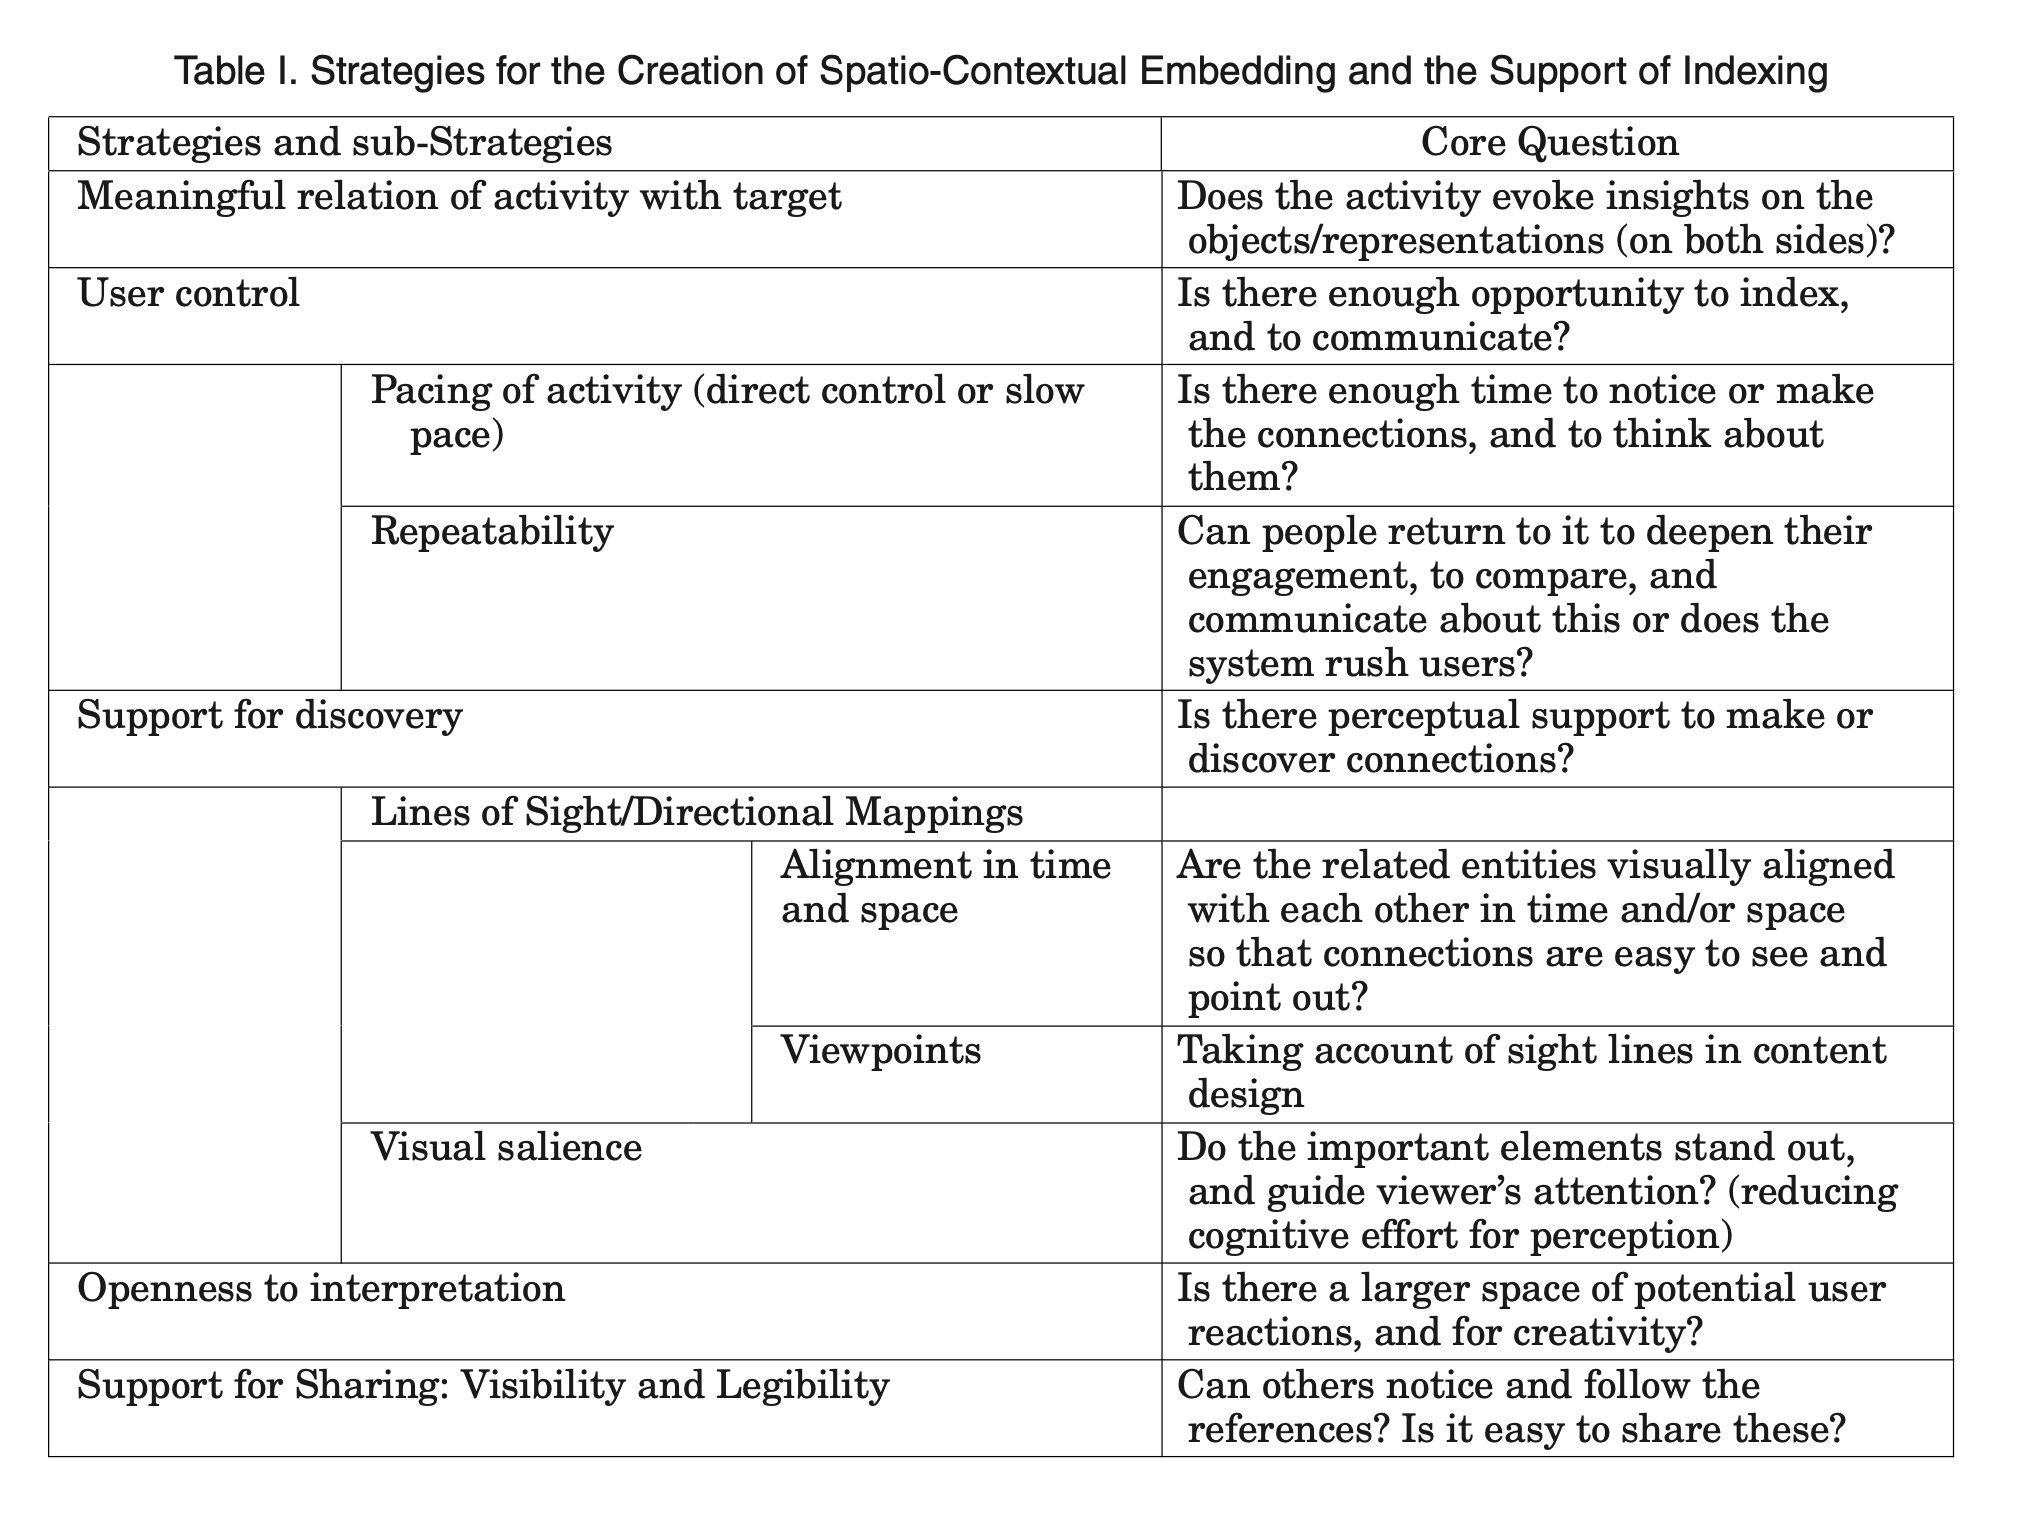
\includegraphics[width=12.5cm]{pictures/strategies.png}
\caption{Sense-making strategies}
\autocite[p. 35]{hornecker_to-and-fro_2016}
\end{figure}

\chapter{\ding{167} A new way of designing for meaningfulness?}
In this chapter it will be showcased how the \emph{Hybrid Place-, Place as Dialogue- and Sense-making strategies} have been operationalised as a theoretical lens to form a proposal of how one can design for meaningfulness. 

This chapter presents the thoughts behind and making of this thesis research contribution: \emph{the framework}.

\section{14 dialogical principles}

The initial problem framing was concerned with designing an installation that addresses sustainability, which triggered a design process and conceptual exploration of sustainability-themes worthy of investigation. Guided by this framing I chose to explore \emph{the relationship between human and nature}. Through literature review (Chapter 2), essay-writings (see appendix) and prototyping (see Chapter 8: Exploring input through plants) I learned that elements, or qualities, (I tend to use the two terms litt hipp som happ). 


Main RQ: How can one design meaningful interactive experiences in
a museum space that addresses sustainability?
answered by: (Sub-RQ): synthesising (or objectifying?) meaningful-
ness as a quality that you can design for in a museum.
through: (Sub-RQ): finding/identifying dialogic relations between
visitor and installation.

Need to defend and justify \emph{why} meaningfulness. 


\begin{figure}[h]
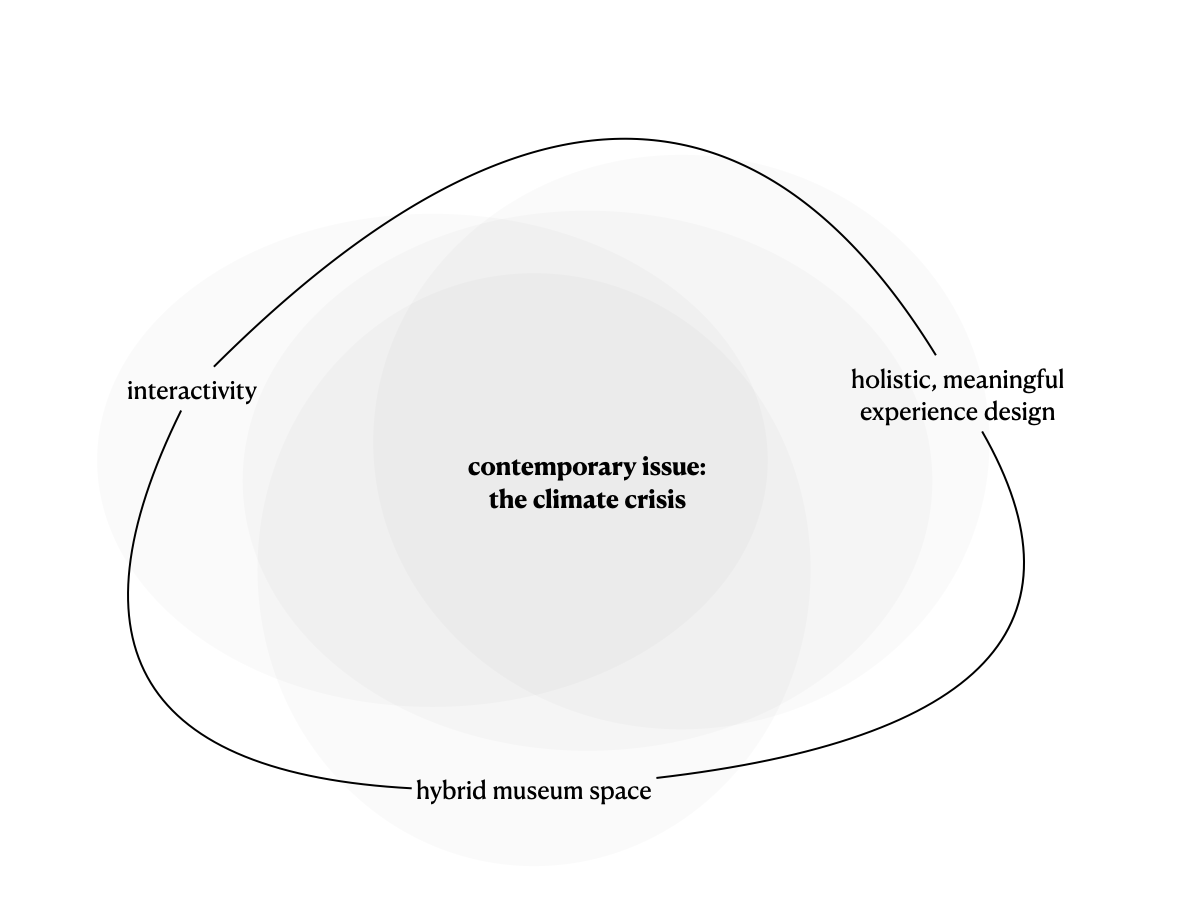
\includegraphics[width=10cm]{pictures/problem_sphere.png}
\caption{My representation of sustainability issues in museums}
\centering
\end{figure}

\begin{figure}[H]
\centering 
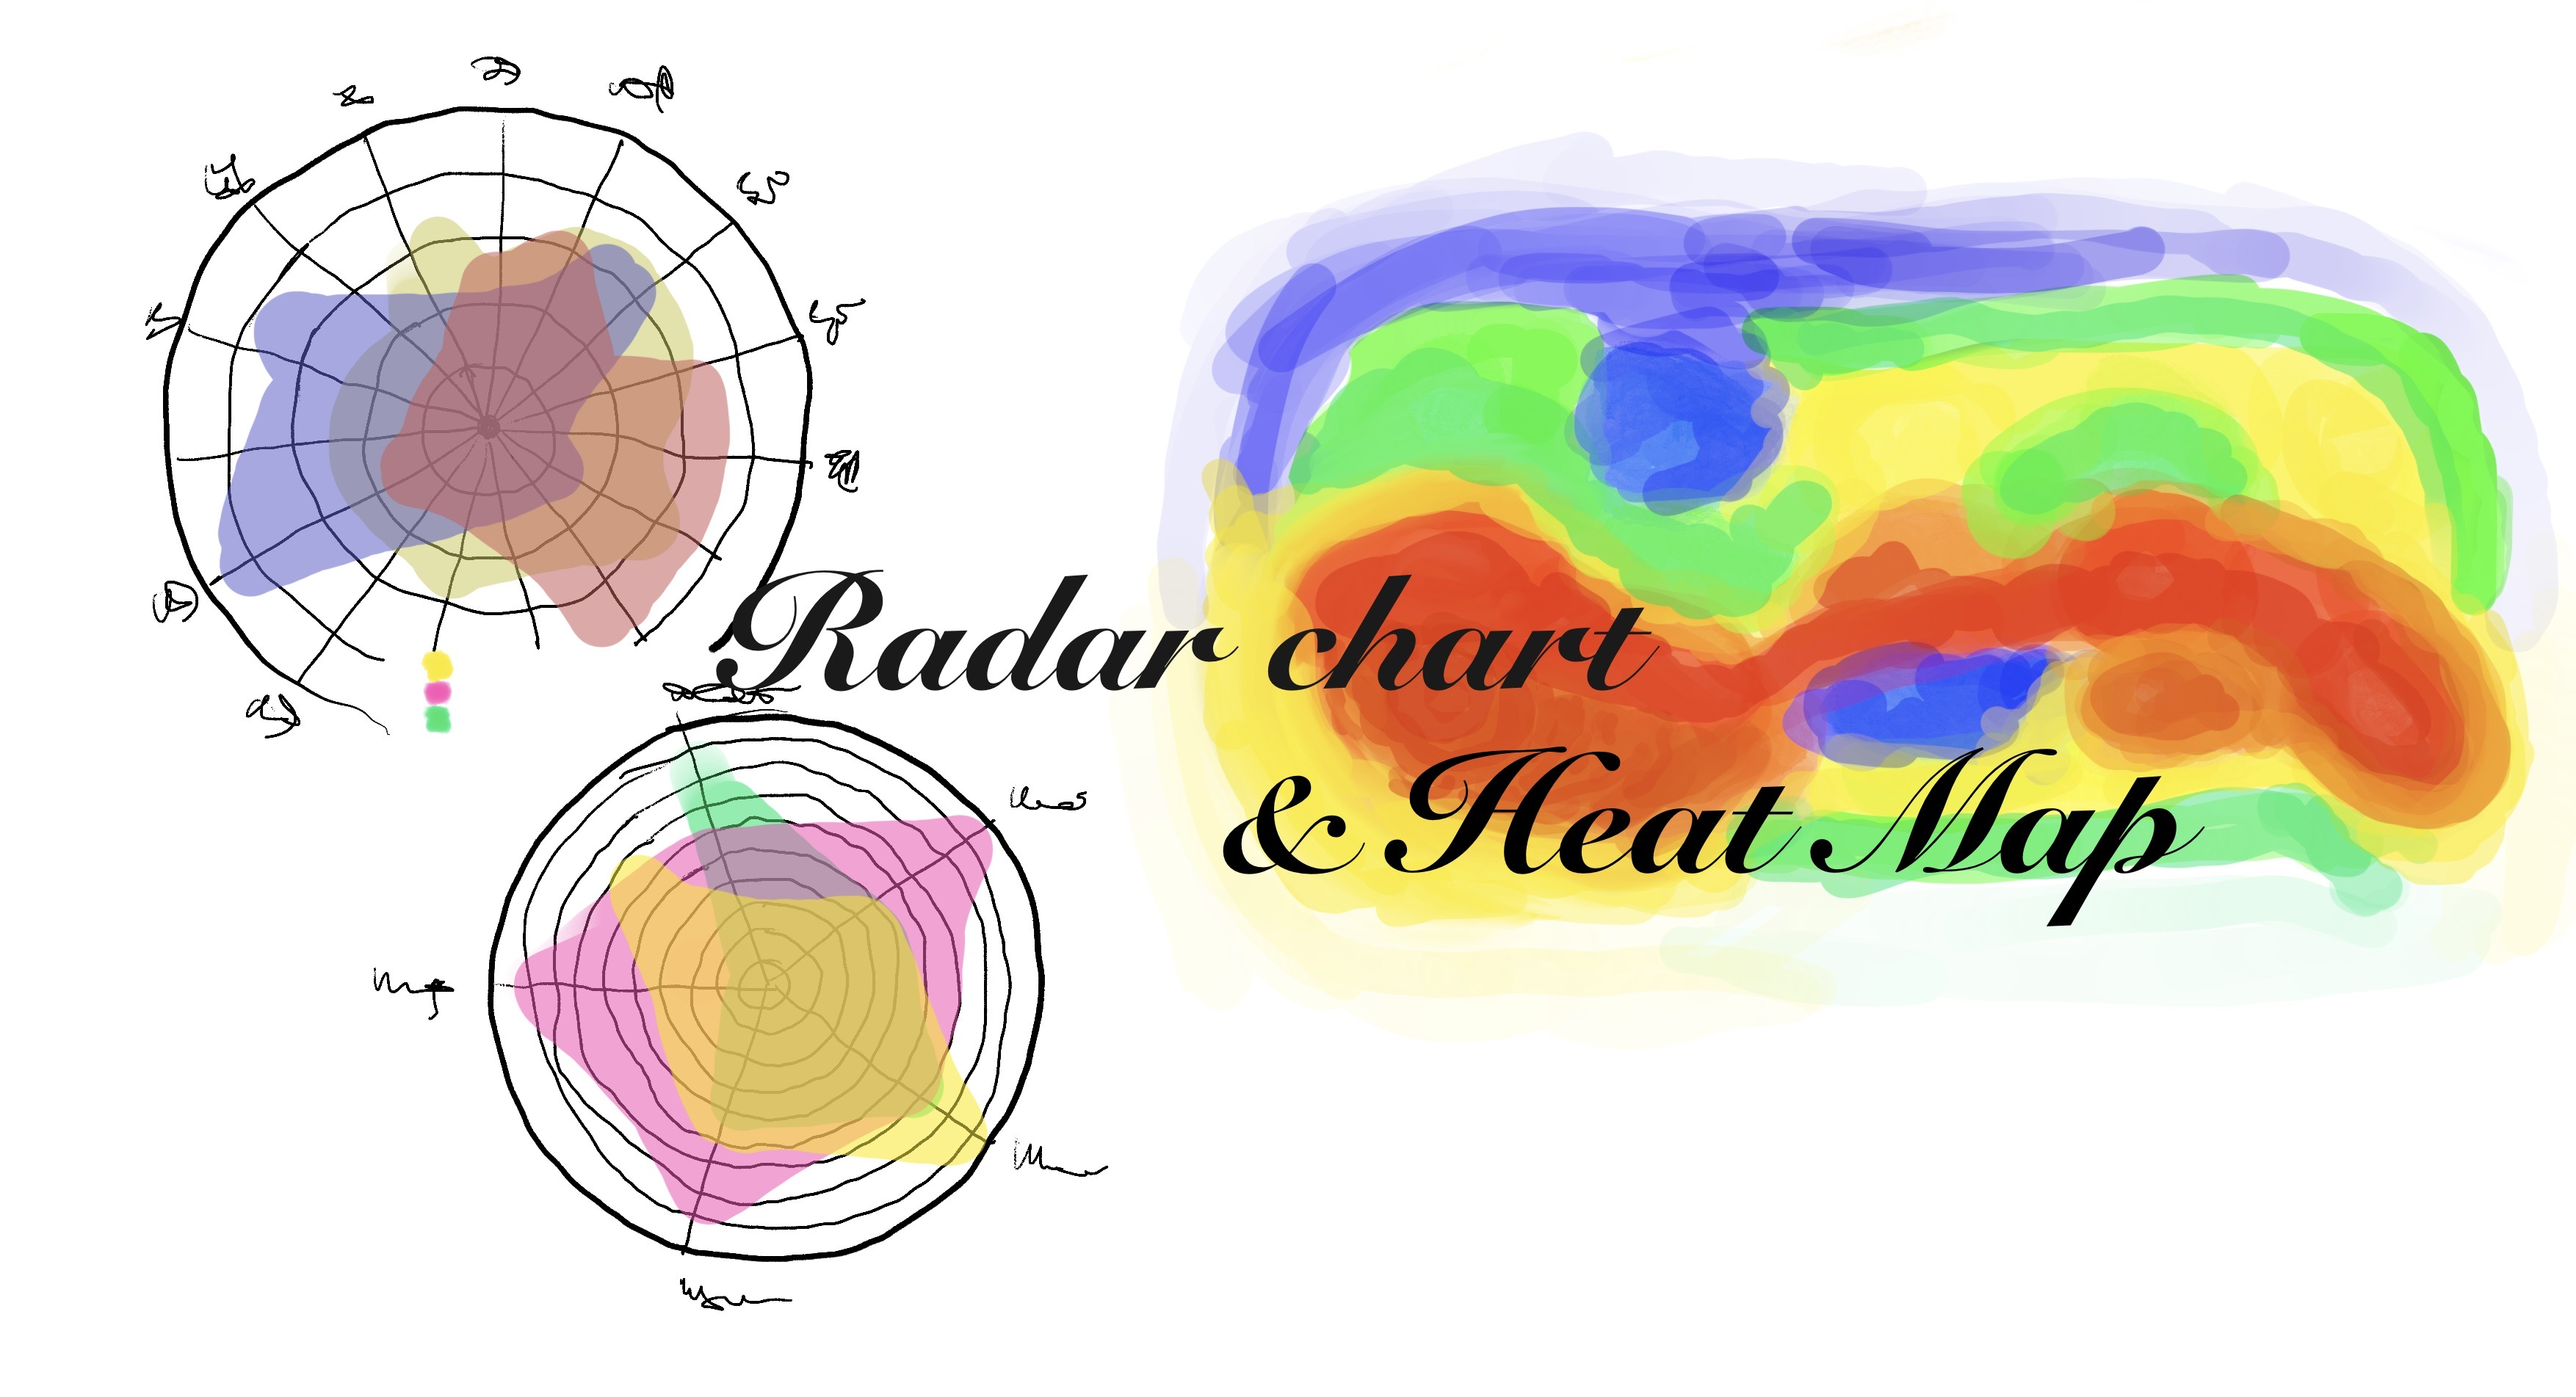
\includegraphics[width=10cm]{pictures/Theory/radar_and_heatmap.jpeg}
\caption{}
\end{figure}




\section{Design for interactive meaningful experiences in a museum}

\begin{figure}[H]
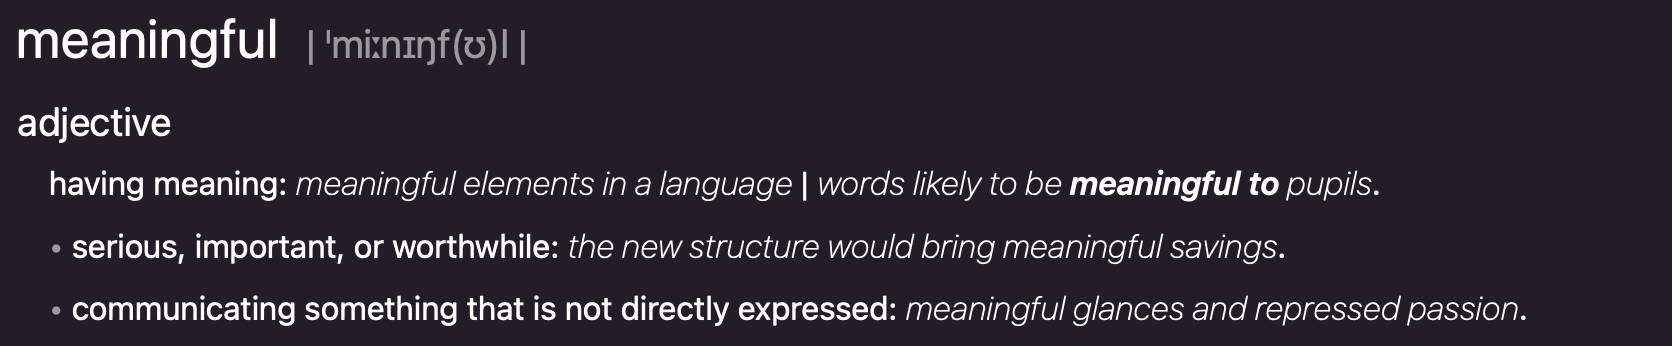
\includegraphics[width=12.5cm]{pictures/background/meaningful.png}
\caption{Meaningfulness}{\autocite{Oxford_dictionary}}
\centering
\end{figure}

The main purpose of this analysis-oriented part is to contribute with knowledge that make visible dialogic qualities between interactive installations and visitor-experience. 

"Finally, by making different things intended to address the same problematic situation, RtD can reveal design patterns \autocite{Alexander_book} around problem framings, around specific interactions, and around how theory can be operationalized" \autocite[p. 178]{zimmerman_research_2014}.


"Each one of these patterns is a morphological law, which established a set of relationships in space, which can always be expressed in the same general form: $X \rightarrow r (A, B, ...)$, which means: Within a context of type X, the Parts A, B, ... are related by the relationship r." \autocite[p. 90]{Alexander_book}.


The way I understand meaningfulness is to compare three approaches; how do the installation fit into the museum agenda? How well does the installation disseminate the message conveyed? and then, in what degree is the interactive elements in the installation dialogic (e.g. how well do they stimulate conversation). In my search for how one can design meaningful interactive experiences in a museum space that addresses sustainability, I propose the theoretical lens I have used to understand and look for meaningfulness in museums. This visualisation illustrates three "edges", of what I mean when I talk about (and synthesise) meaningfulness. 


\begin{figure}[h]
\centering 
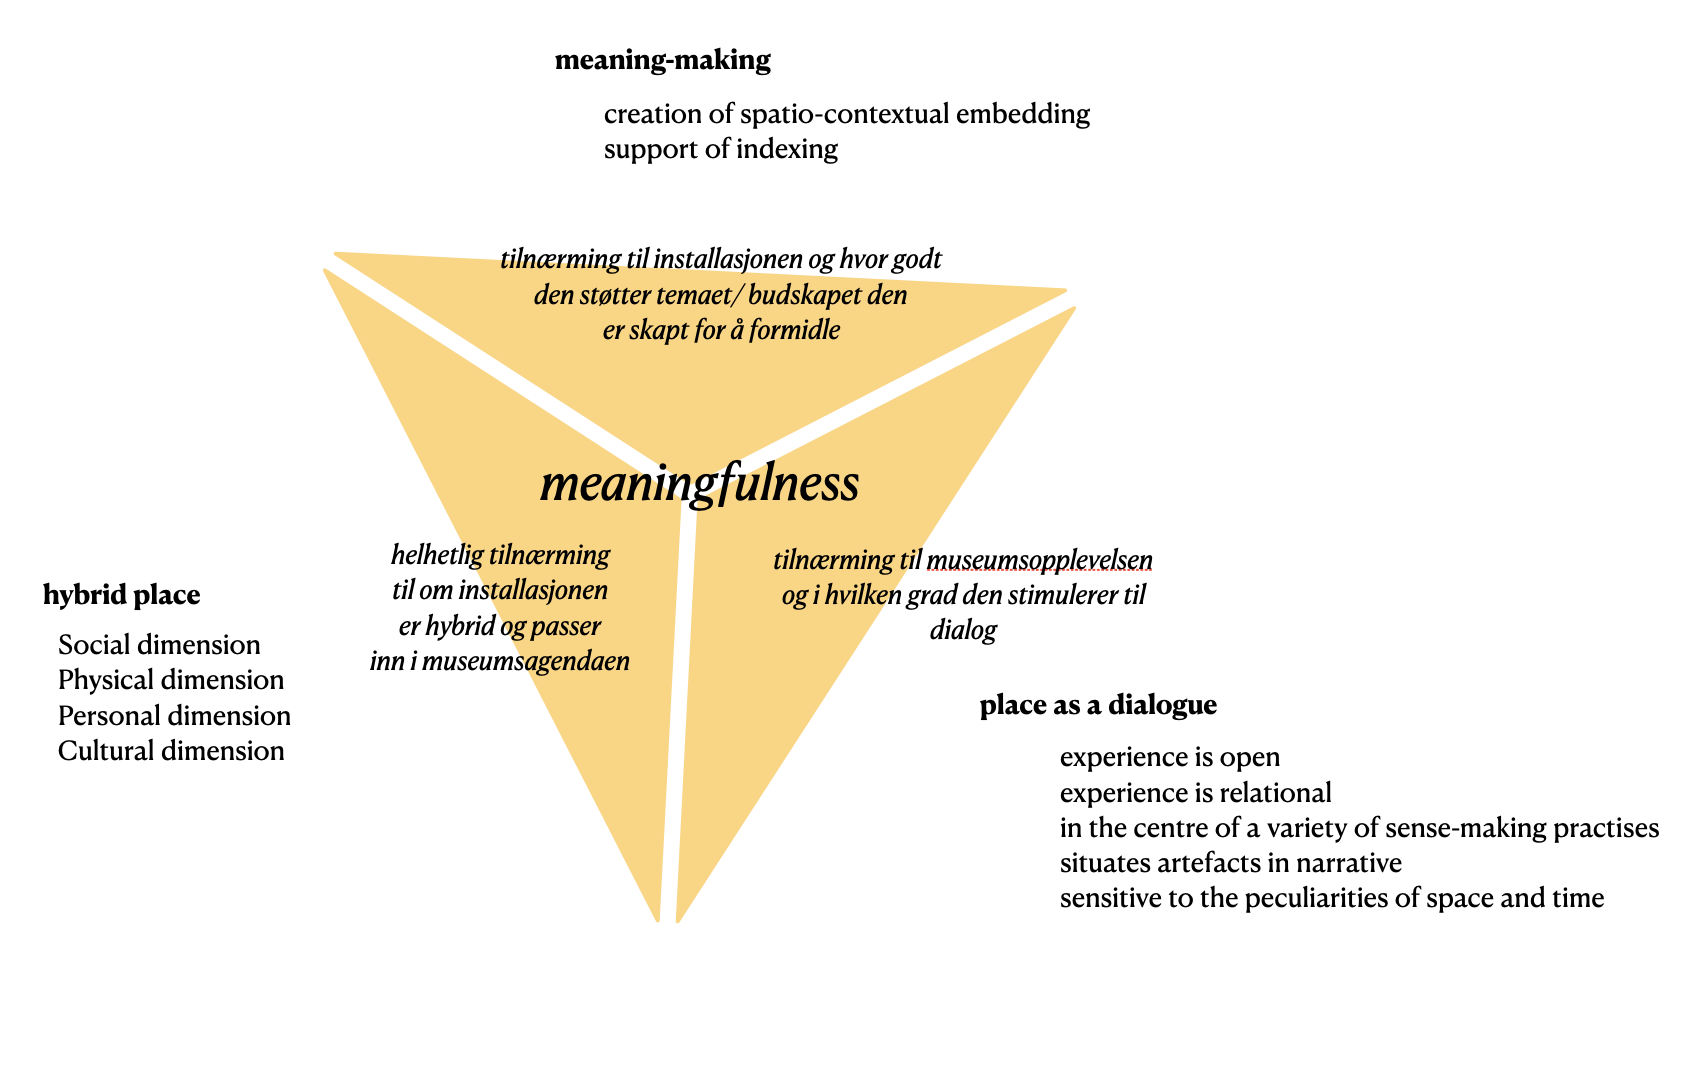
\includegraphics[width=13cm]{pictures/meaningfullness_triangle.png}
\caption{}
\end{figure}


\begin{figure}[h]
\centering 
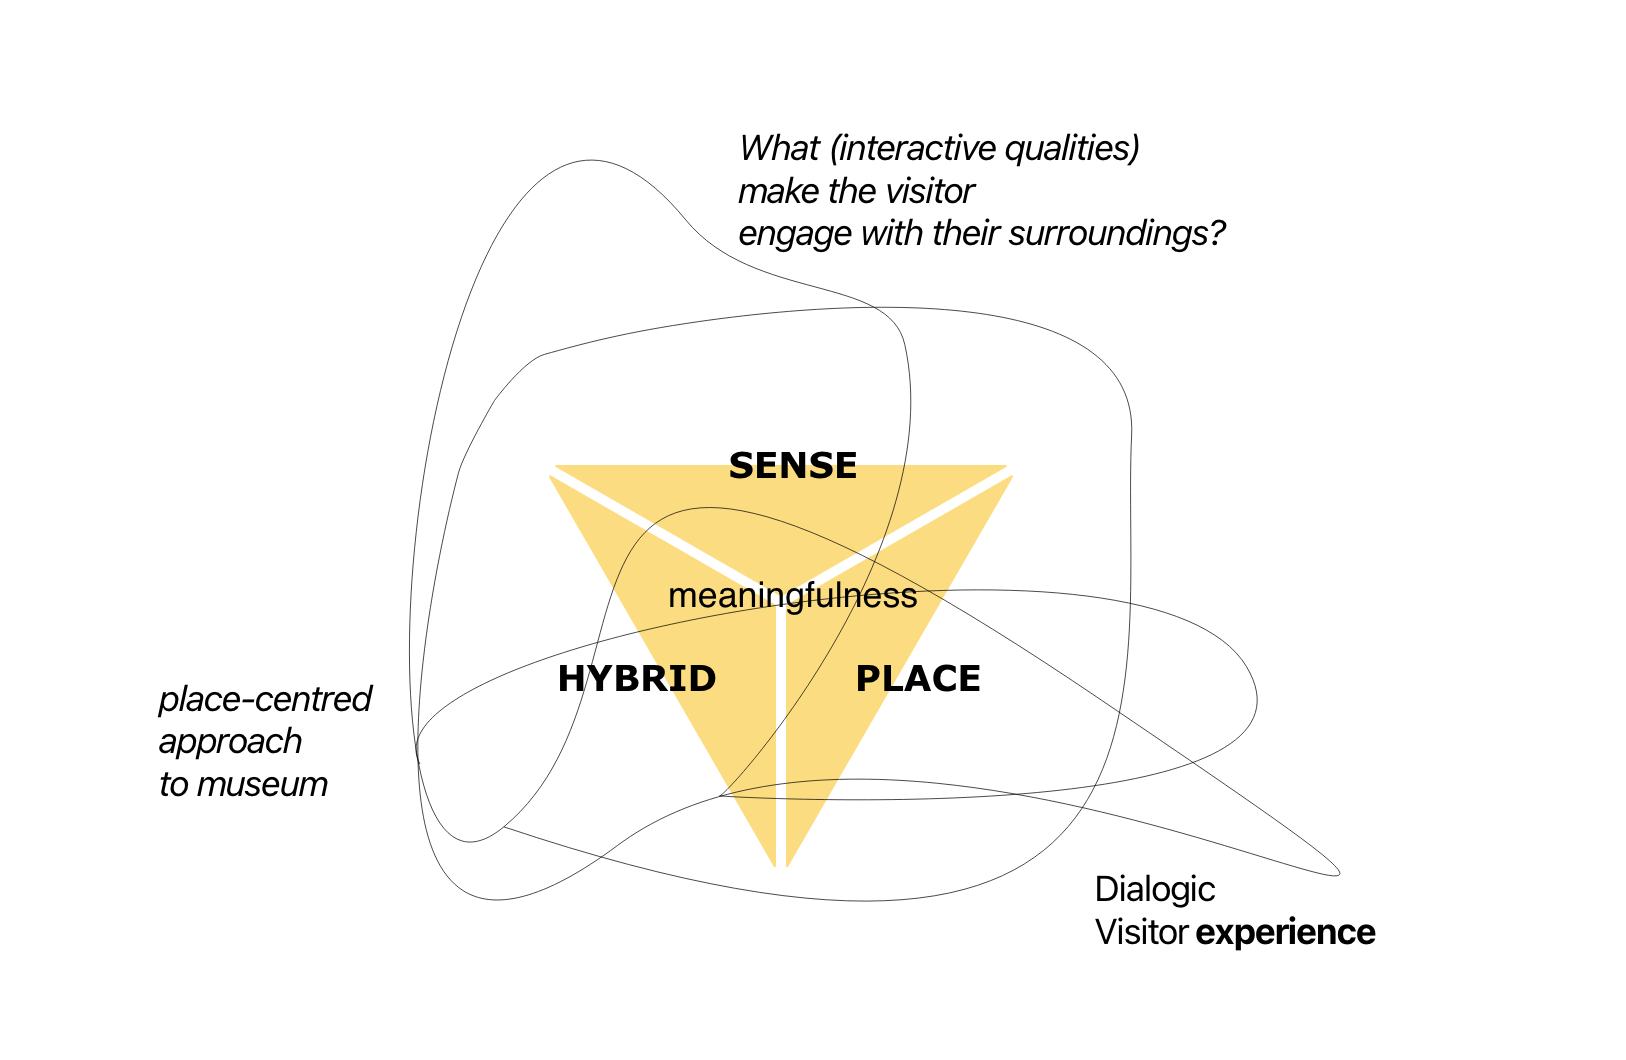
\includegraphics[width=13cm]{pictures/Theory/early_iteration_framework.png}
\caption{}
\end{figure}

\begin{figure}[h]
\centering 
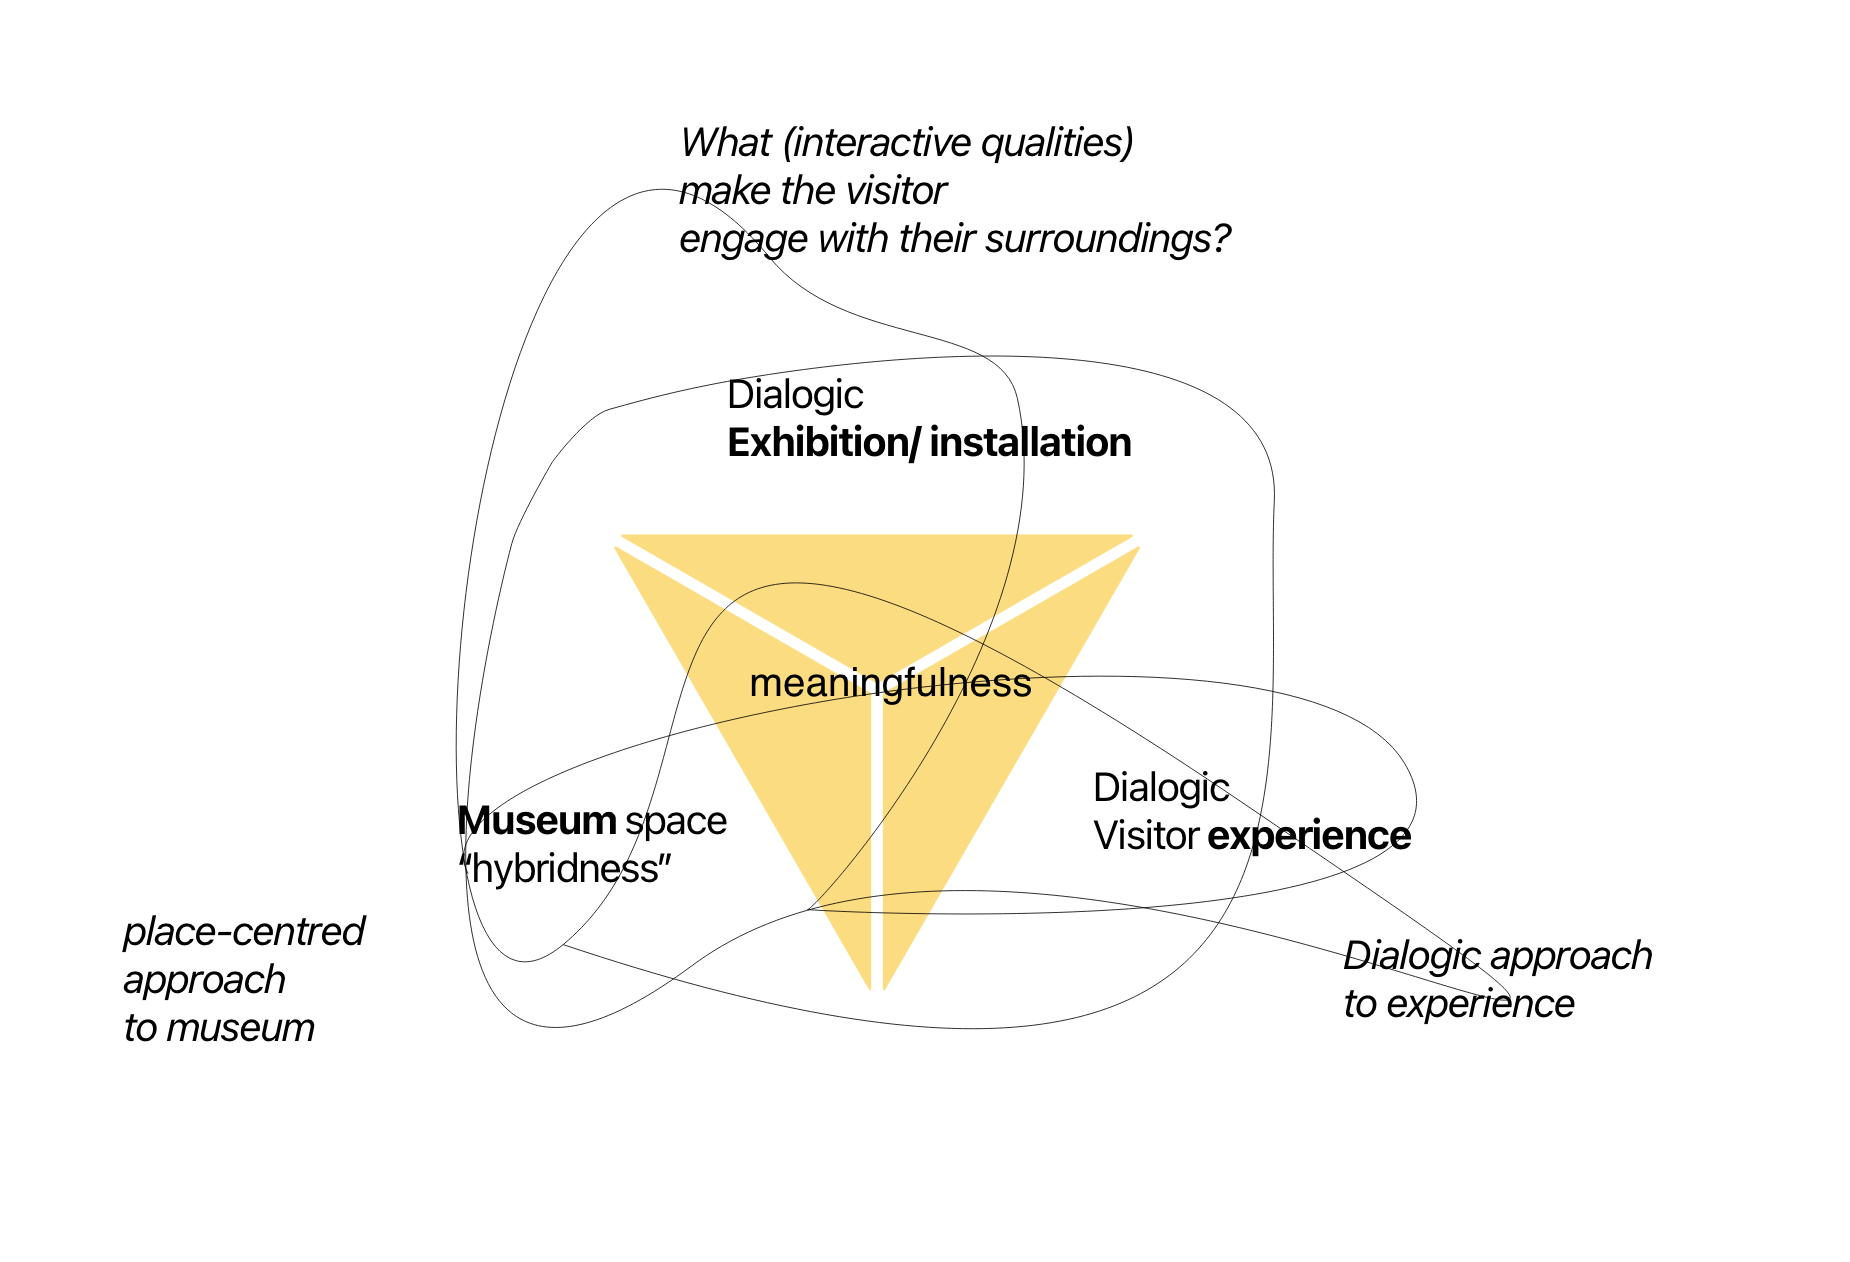
\includegraphics[width=13cm]{pictures/Theory/meaningfulness_triangle.png}
\caption{}
\end{figure}

The visualisation illustrates my definition of meaningfulness as a quality that you can design for. The triangle is an attempt to showcase what "aspects" I borrow/build upon from each respective theoretical framework, and then how together they fulfill three dimensions to how meaningfulness can be understood (interpreted?).
From the Hybrid Place framework I borrow four dimensions; the \emph{physical, social, personal and cultural}, as a way to portray/ map out the installation in relation to its environments. I see it as a holistic approach to judge the "hybridness" of the installation in relation to its surrounds, so that I can see in what dimensional direction the potential meaningful relation between visitor and installation could be.

The practical application of this analytical tool is something like this (the tables underneath), where I have plotted in the different installations and exhibitions to their respective tables. A thoruough walkthrough of the analysis is accounted for in Chapter 9: Analysis.



\part{Design Process}

\chapter{\ding{167} Methodology}
\section{About the process }

August - December 2020, the first semester on the master degree was spent finding a supervisor and deciding/ orienting on what I wanted to write about. The second semester was for the most part theoretical, getting to know the museum domain and working on the research question and angle for the thesis. Started 

\begin{figure}[h]
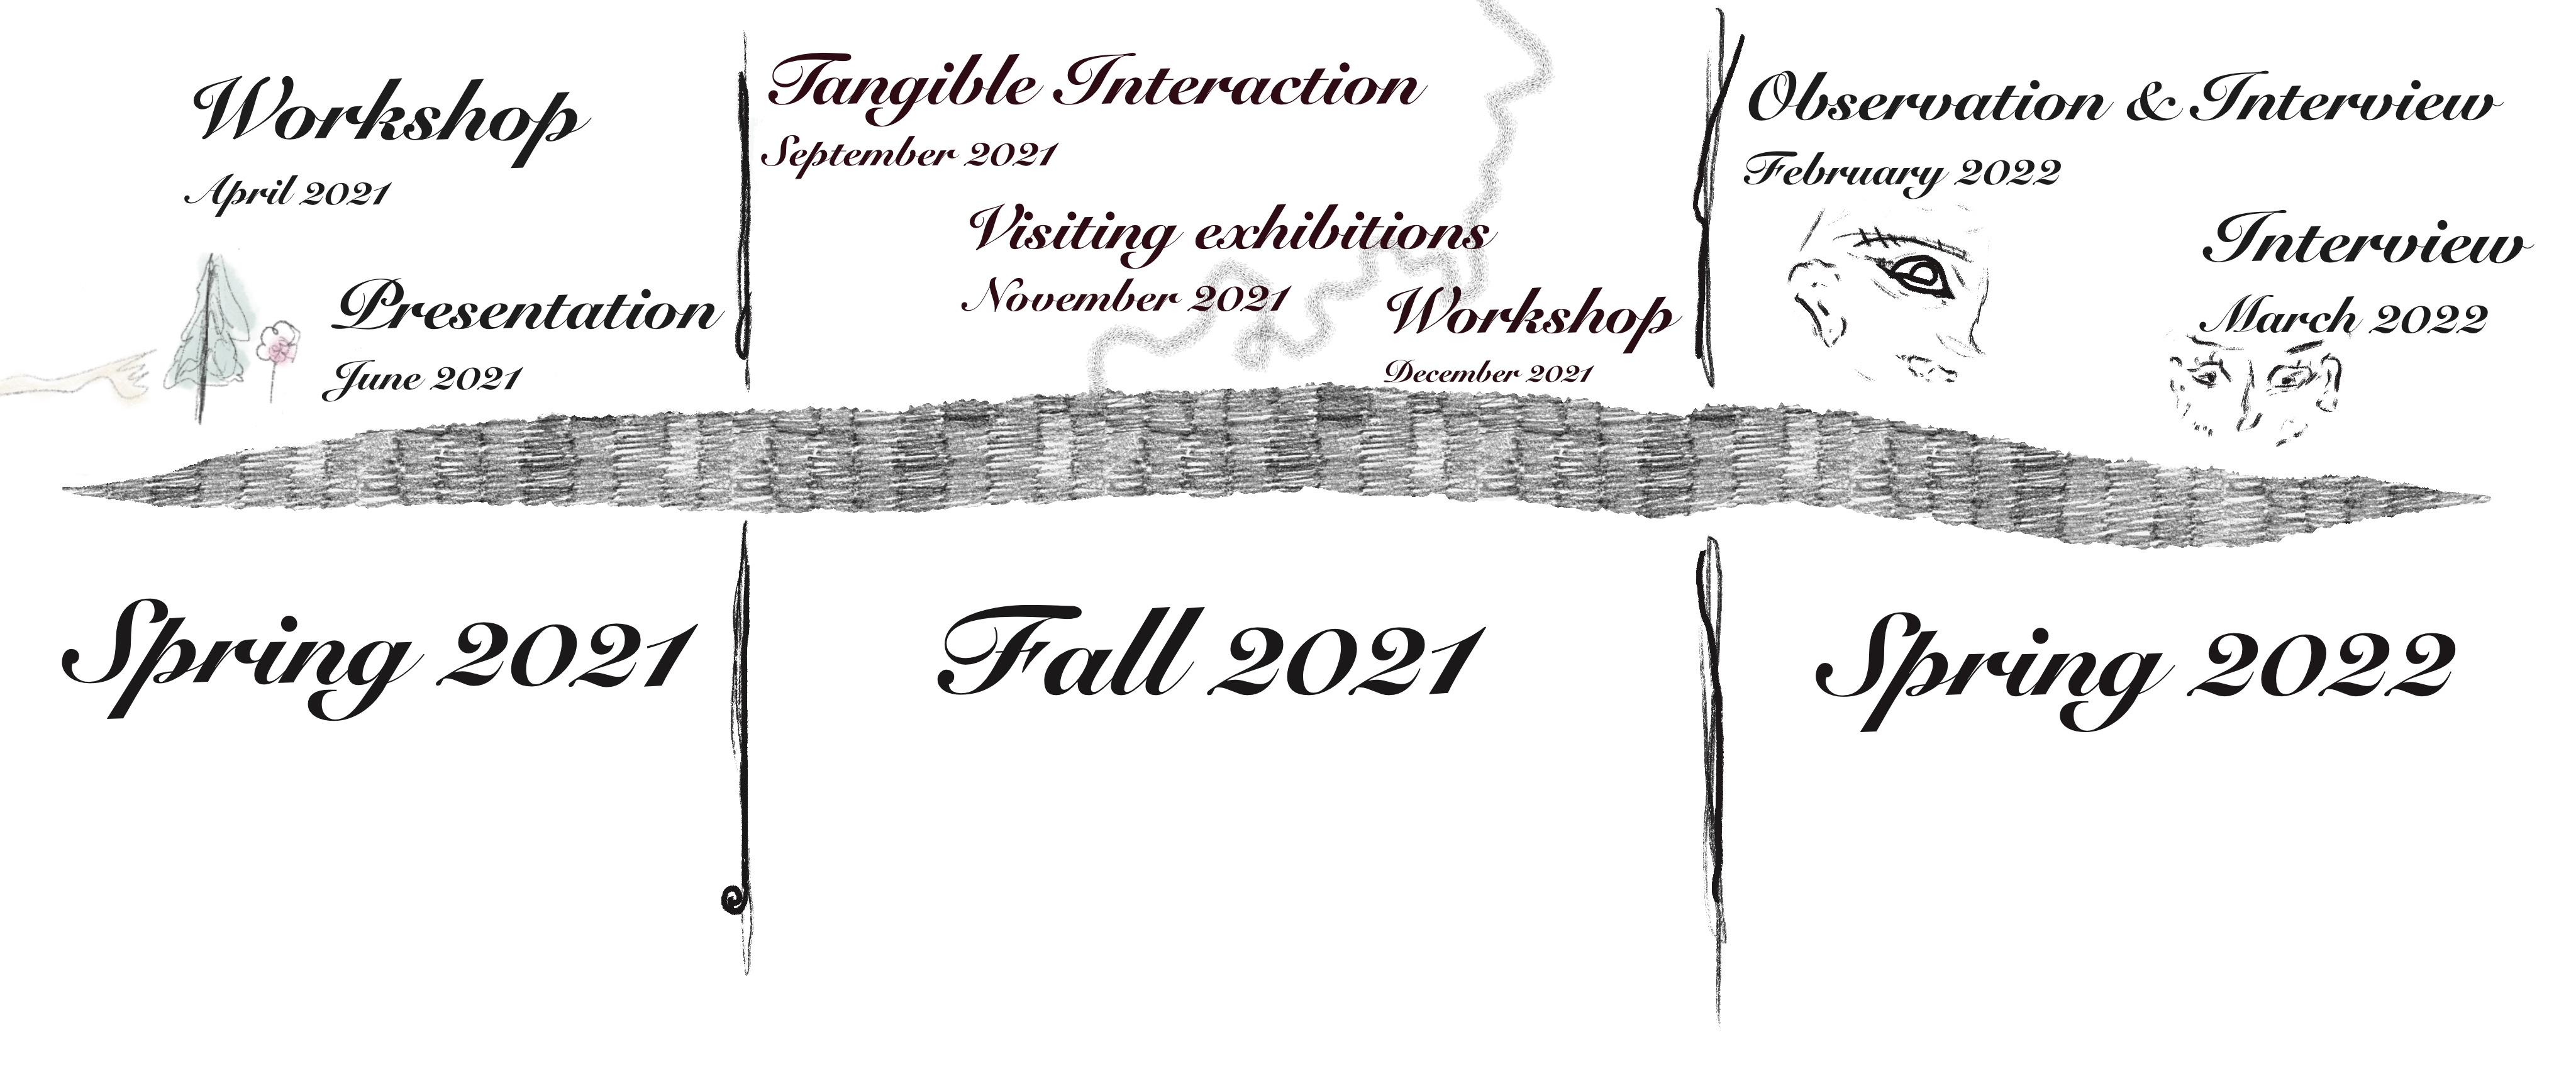
\includegraphics[width=13cm]{pictures/timeline.jpg}
\centering 
\end{figure}


The dataset that I/we have done for this thesis is as following:
\begin{itemize}
    \item Workshop with stakeholders from Klimahuset, april 21
    \item Presentation w/ prototypes at Klimahuset, june 21
    \item Visited 5 different interactive exhibitions, fall 21
    \item Energy visualisation workshop with Qi-installation
    \item Observation of 2 school children classes in Klimahuset, february 22
    \item Interview with two of Klimahuset Docents, february 22
    \item Interview and observation w/ concept developer at Munch, march 22
    \item Analysis/ theorethical framework workshop sessions
\end{itemize}

\section{The dataset}
Over the course of this thesis, my research buddies and I have visited in total 10 exhibitions from 7 different museums in Oslo. From these museum visits, we have documented 22 interactive installations that forms the dataset used for analysis and similar investigations in our respective thesis's. 

\begin{figure}[H]
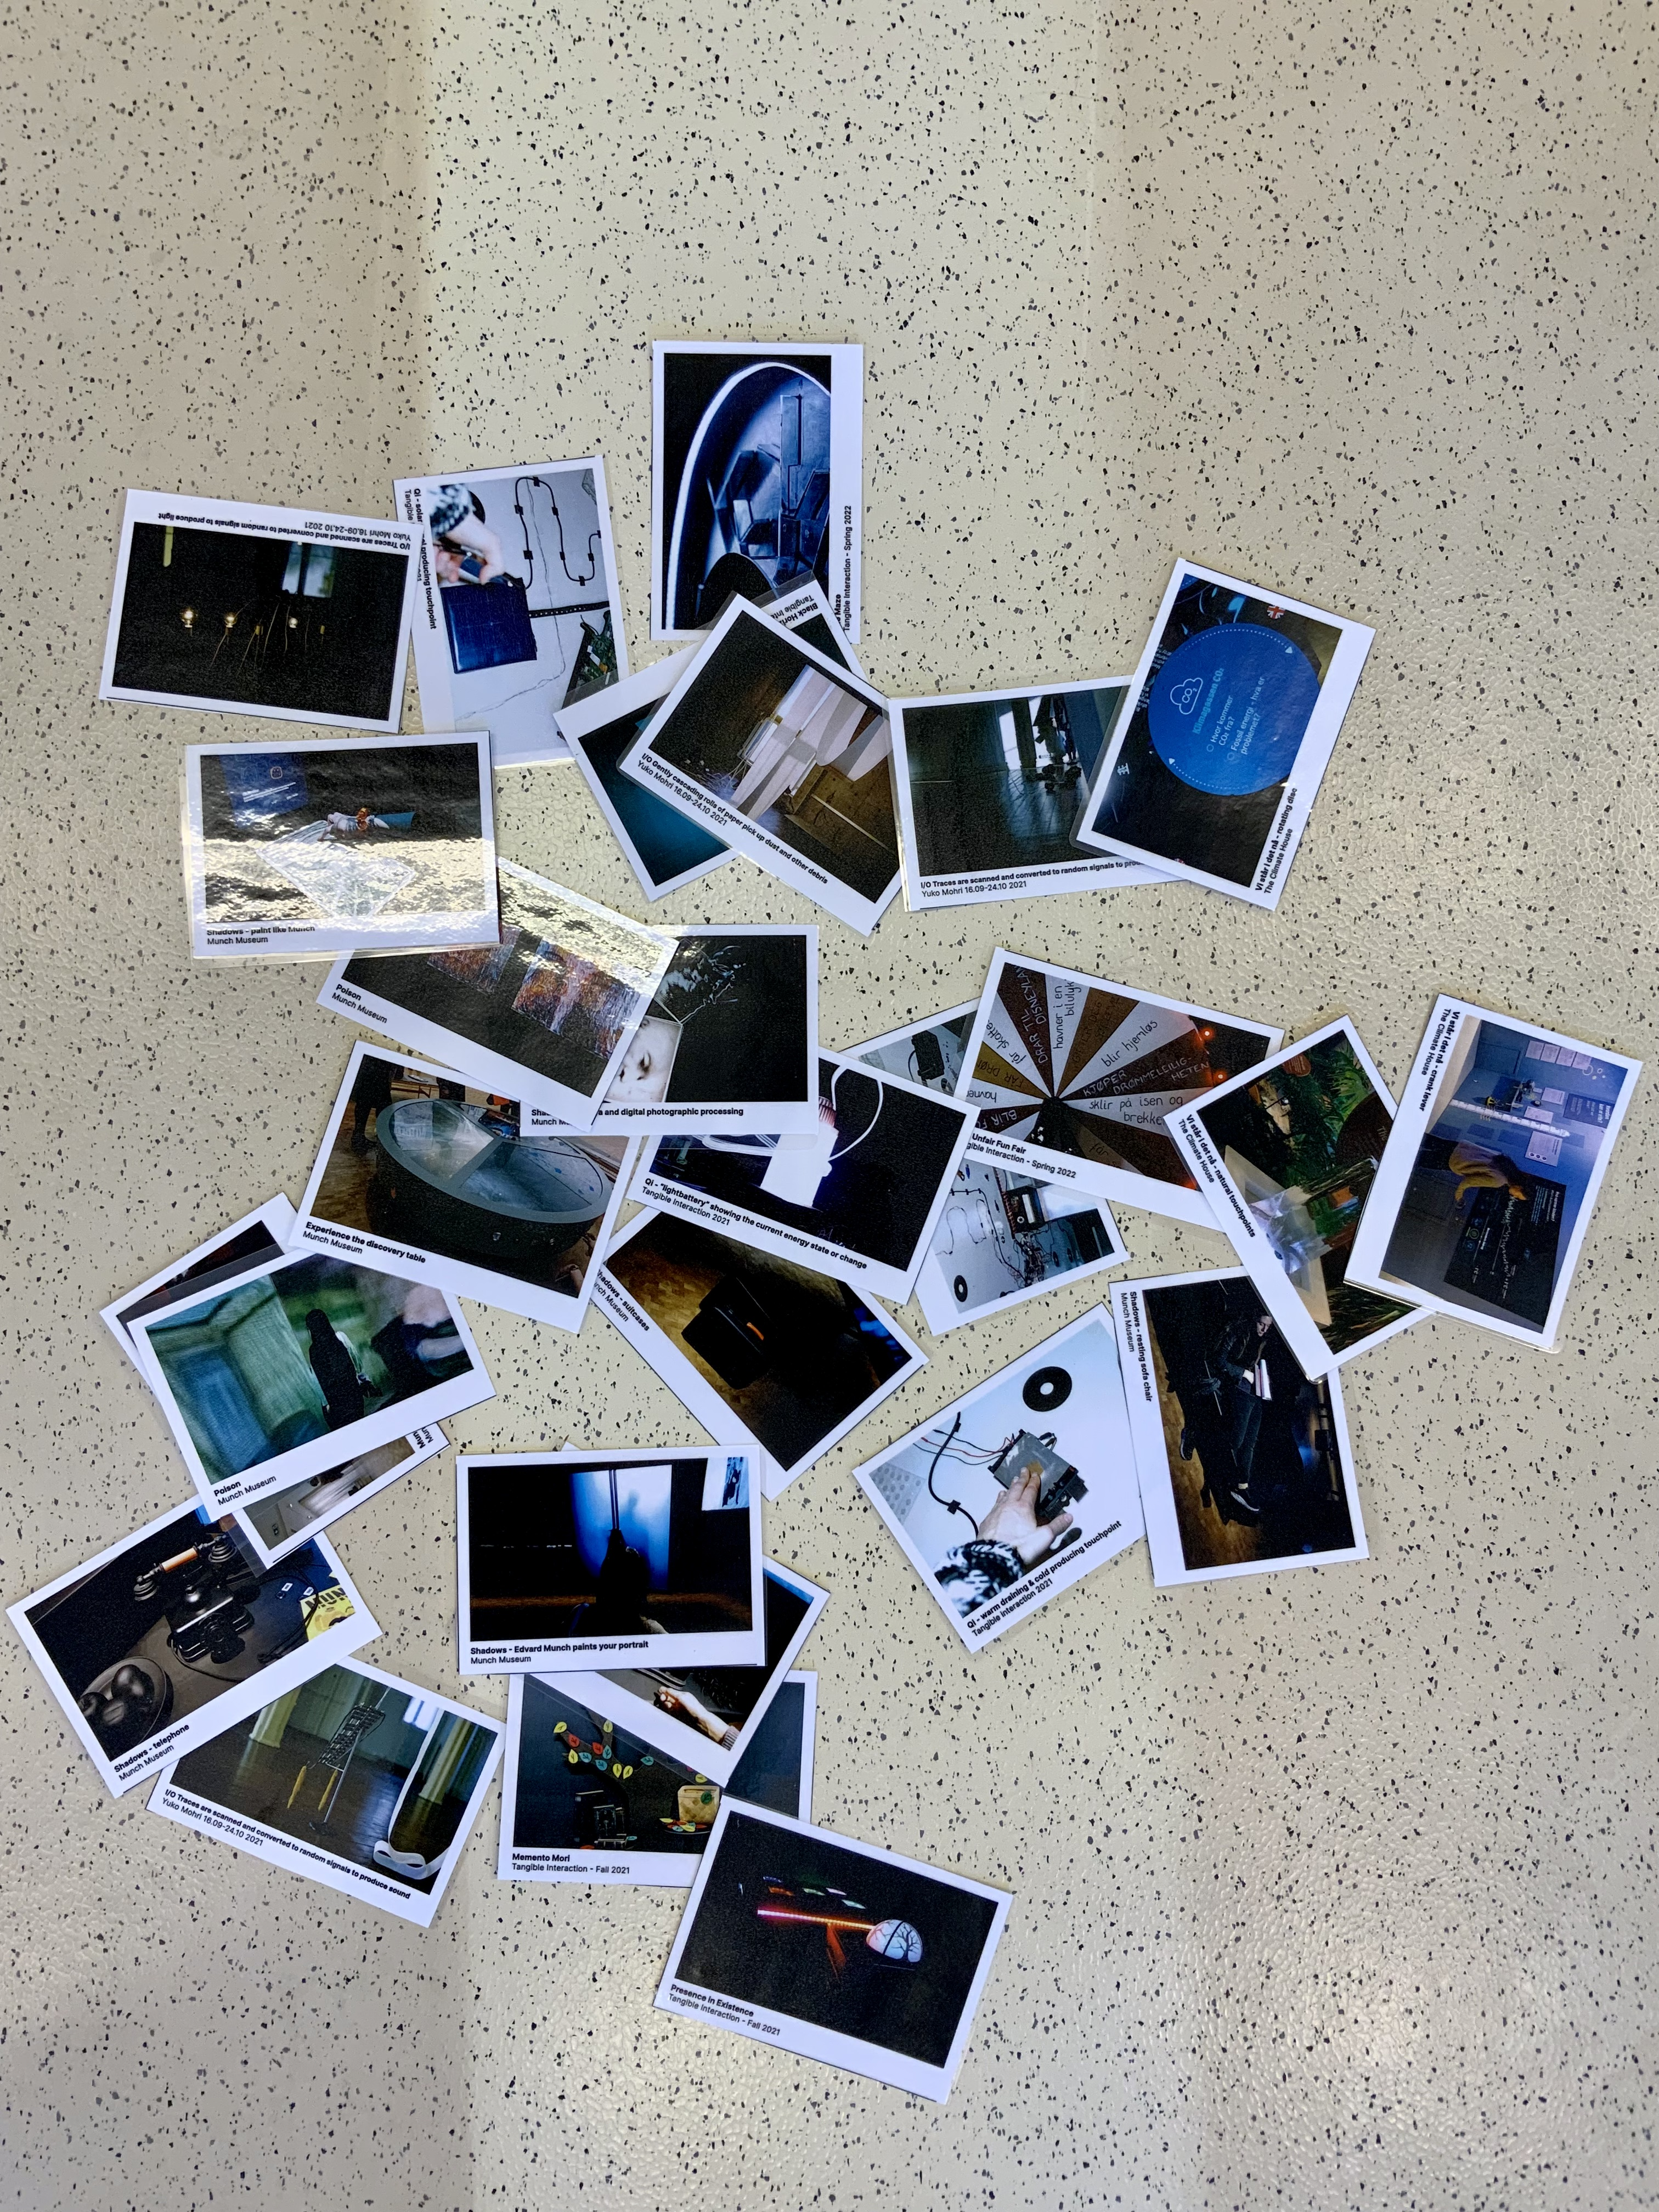
\includegraphics[width=12cm]{pictures/dataset/datasett_oversikt.jpeg}
\centering 
\end{figure}

I think this is basic qualitative analysis?

Måten jeg har gått frem på ved bruk av dette datasettet, sett opp mot mine utvalgte teorier, har vært en form for deduktiv systematisk prosess. Det vil si at jeg til å begynne med har systematisert og kategorisert installasjonene opp mot hver teori; feks som jeg har gjort her fra en av de interaktive installasjonene på klimahuset haar jeg

\subsection{"data laundering"}
Write out:
\begin{itemize}
    \item explain why munch shadows is analysed as one. and only weighted as one. and how that affects the dataset.
    \item discuss how the amount of tangible installations affect the dataset
    \item discuss the analog-tangible vs interactive-tangible installations (ice cube, munch peepholes and discovery table)
\end{itemize}

\begin{figure}[H]
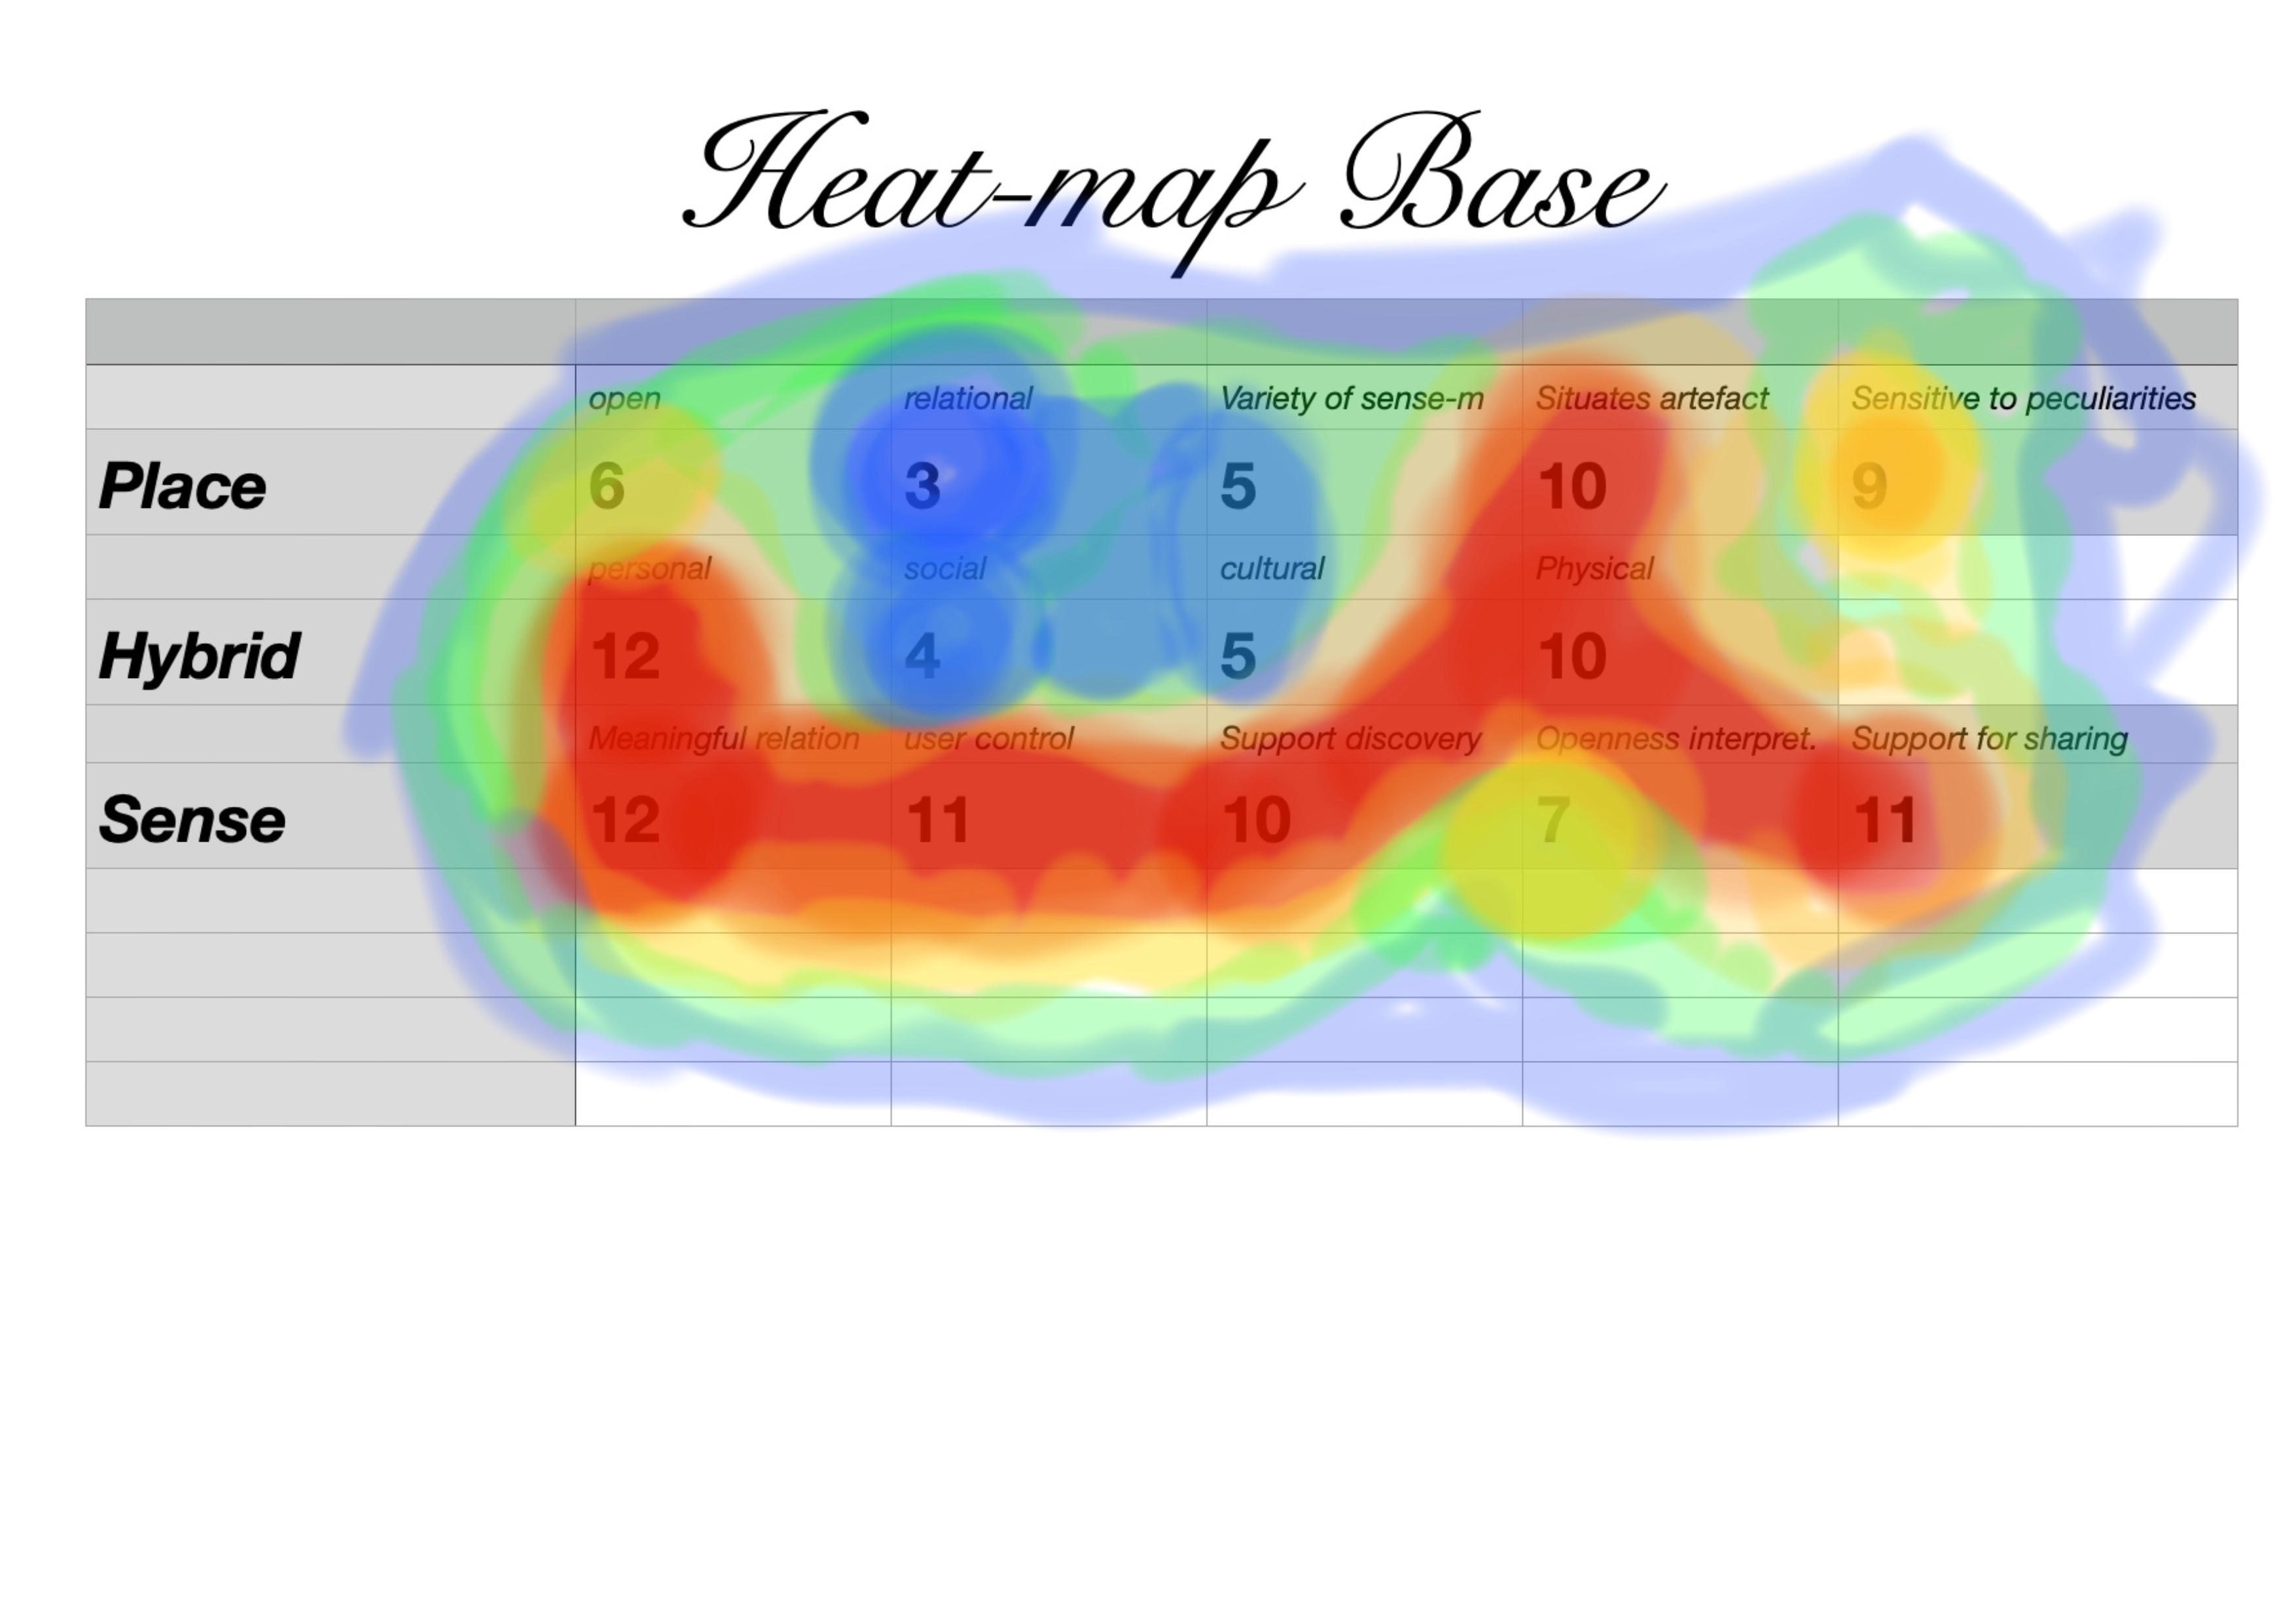
\includegraphics[width=11cm]{pictures/dataset/heatmap.jpg}
\centering 
\end{figure}


\section{First iteration: getting to know the bigger picture}

I started the first analytical iteration by sorting the dataset into the three theories I base my understanding of meaningfulness on; \emph{Hybrid place, place as a dialogue} and \emph{Sense-making strategies}. I made one table for each theory, where the frameworks's principles/ and dimensions formed the columns and the 22 different installations the rows. I then went through each installation and plotted in whether or not the installation fulfilled the principle/ dimension. Categorising it this way opened up for looking at the dataset in correlation with each theory separately, making it possible to see overall trends in the dataset according to the theories. Another


respective theory from a birds-eye, holistic, perspective, but it will also work as a quick-reference guide for the second analysis iteration when I'm trying to merge the three theories and/ or finding new relationships between the data across the theories.

The categorisation of the data is highly subjective, but theoretically grounded, based on my personal experience with- and interpretation of the installations and knowledge of the museum institution the installation was part of. I have also chosen to merge all the Munch - \emph{Shadows} installations as one, because they are a part of the same exhibition and do not differ in their interactive qualities. Because of this, the dataset used for this analysis shrinked from 22 to 16. This choice of merging the \emph{Shadows} installations was made in the process of fitting the installations into the theory's principles/ dimensions, when I saw that they all checked the same boxes. 


\begin{figure}[H]
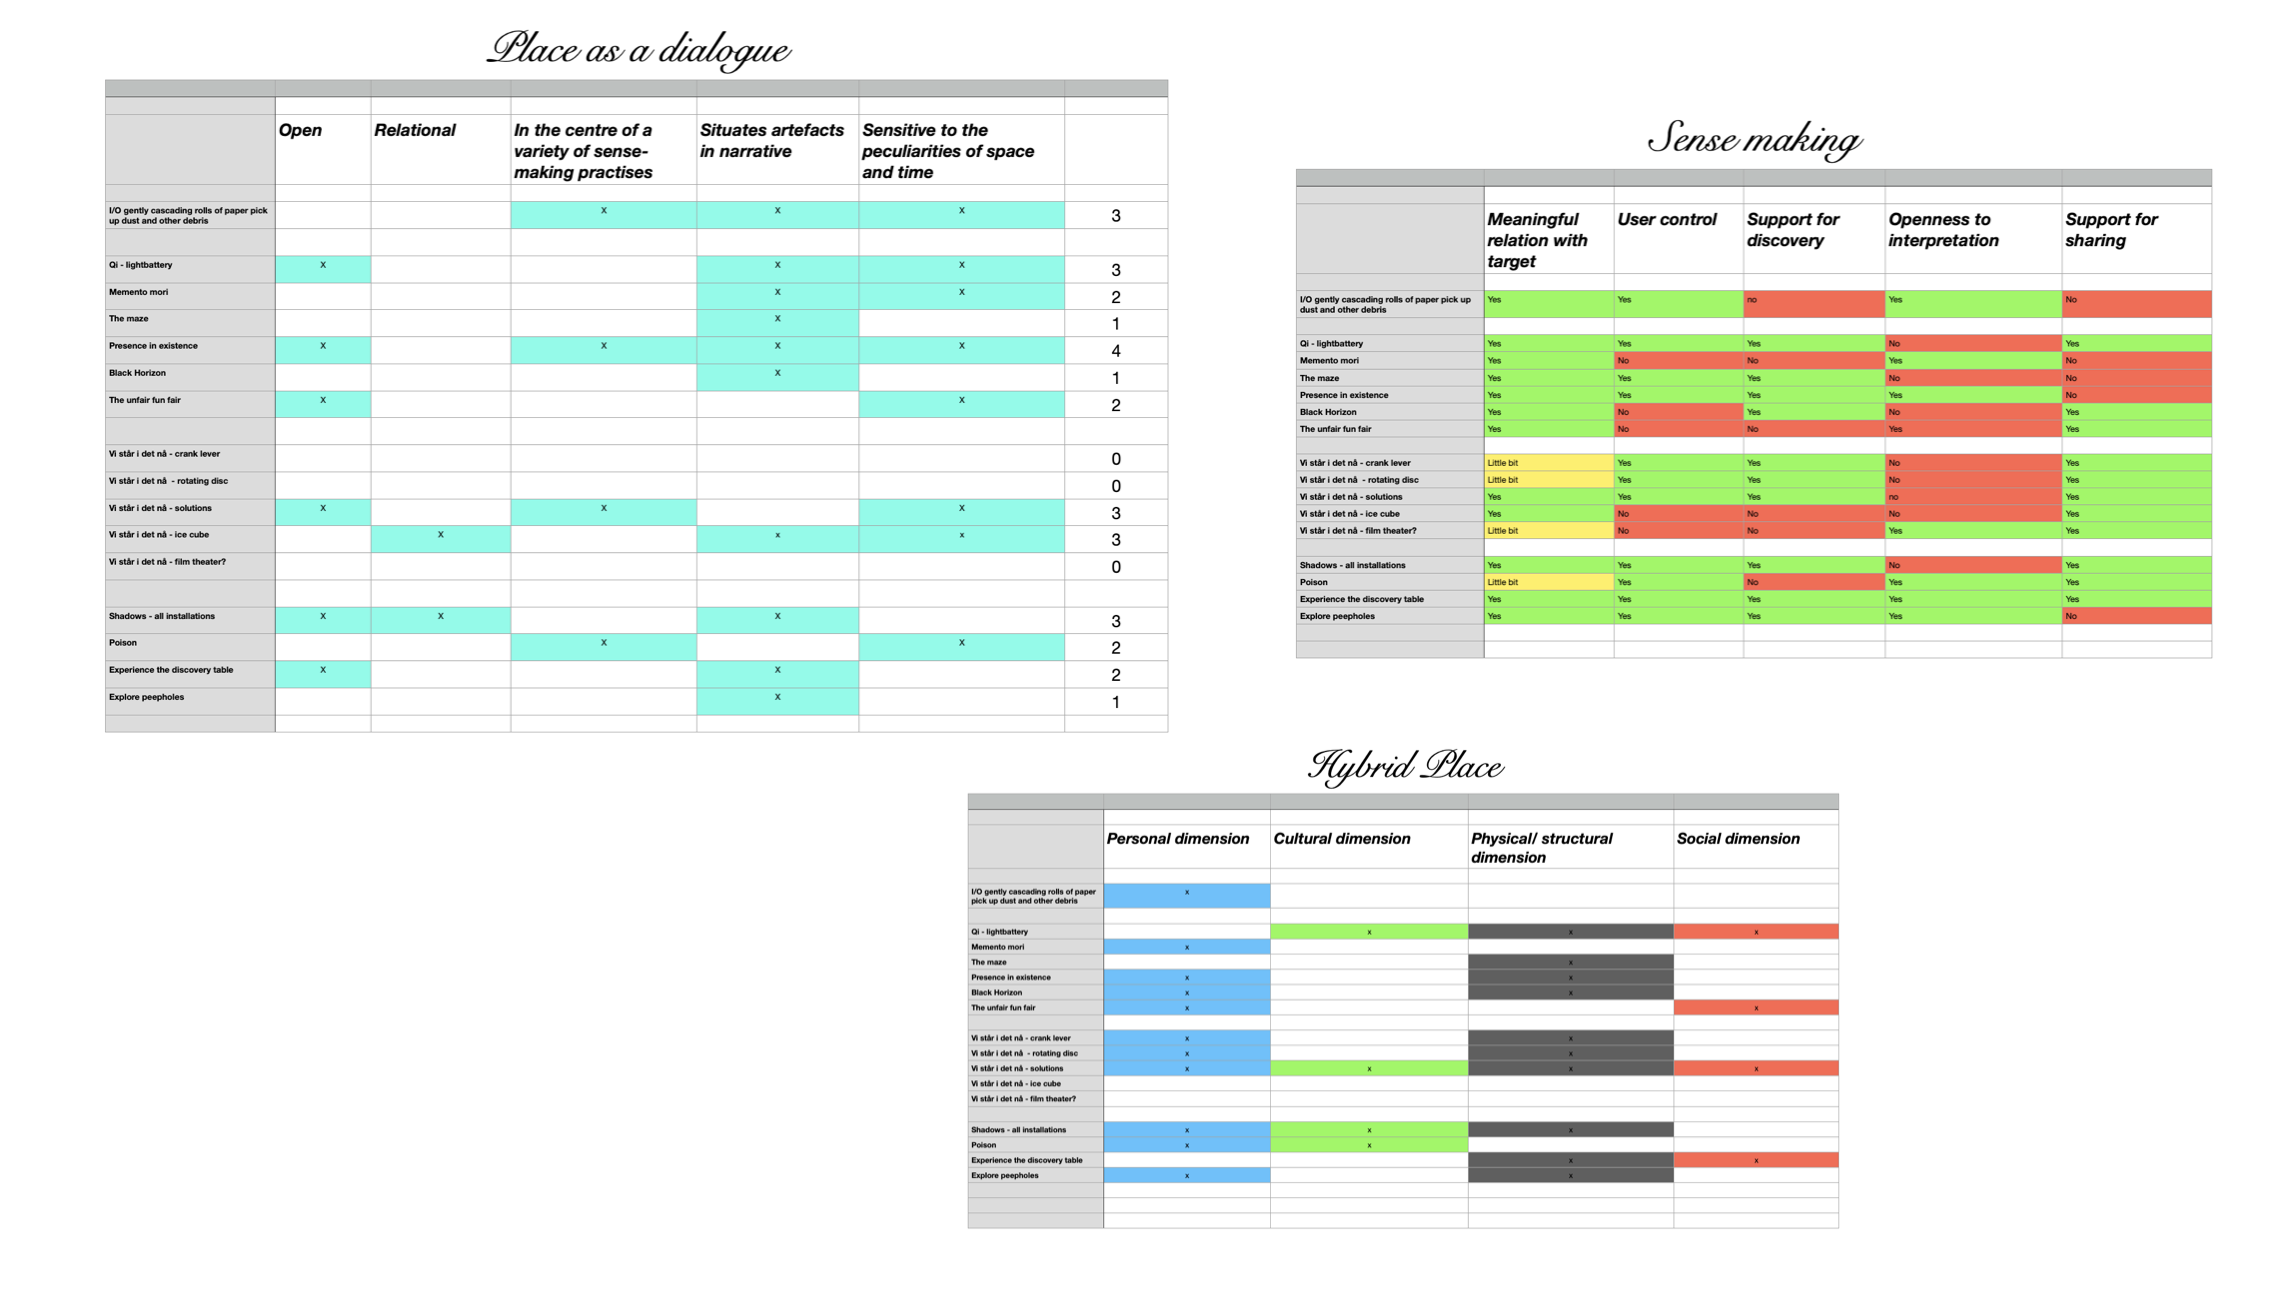
\includegraphics[width=13cm]{pictures/dataset/analysis_tables.png}
\centering 
\end{figure}

After mapping the installations in the tables, it opened up for crunching the first numbers. In this iteration I want to see the dataset from a holistic view. Abstracting from the details and seeing how the installations map up in the bigger picture. To do this I needed a diagram that could compare the different principles up against eachother. I chose to create radar charts to do this, and made a radar chart for each theory. 

\begin{figure}[H]
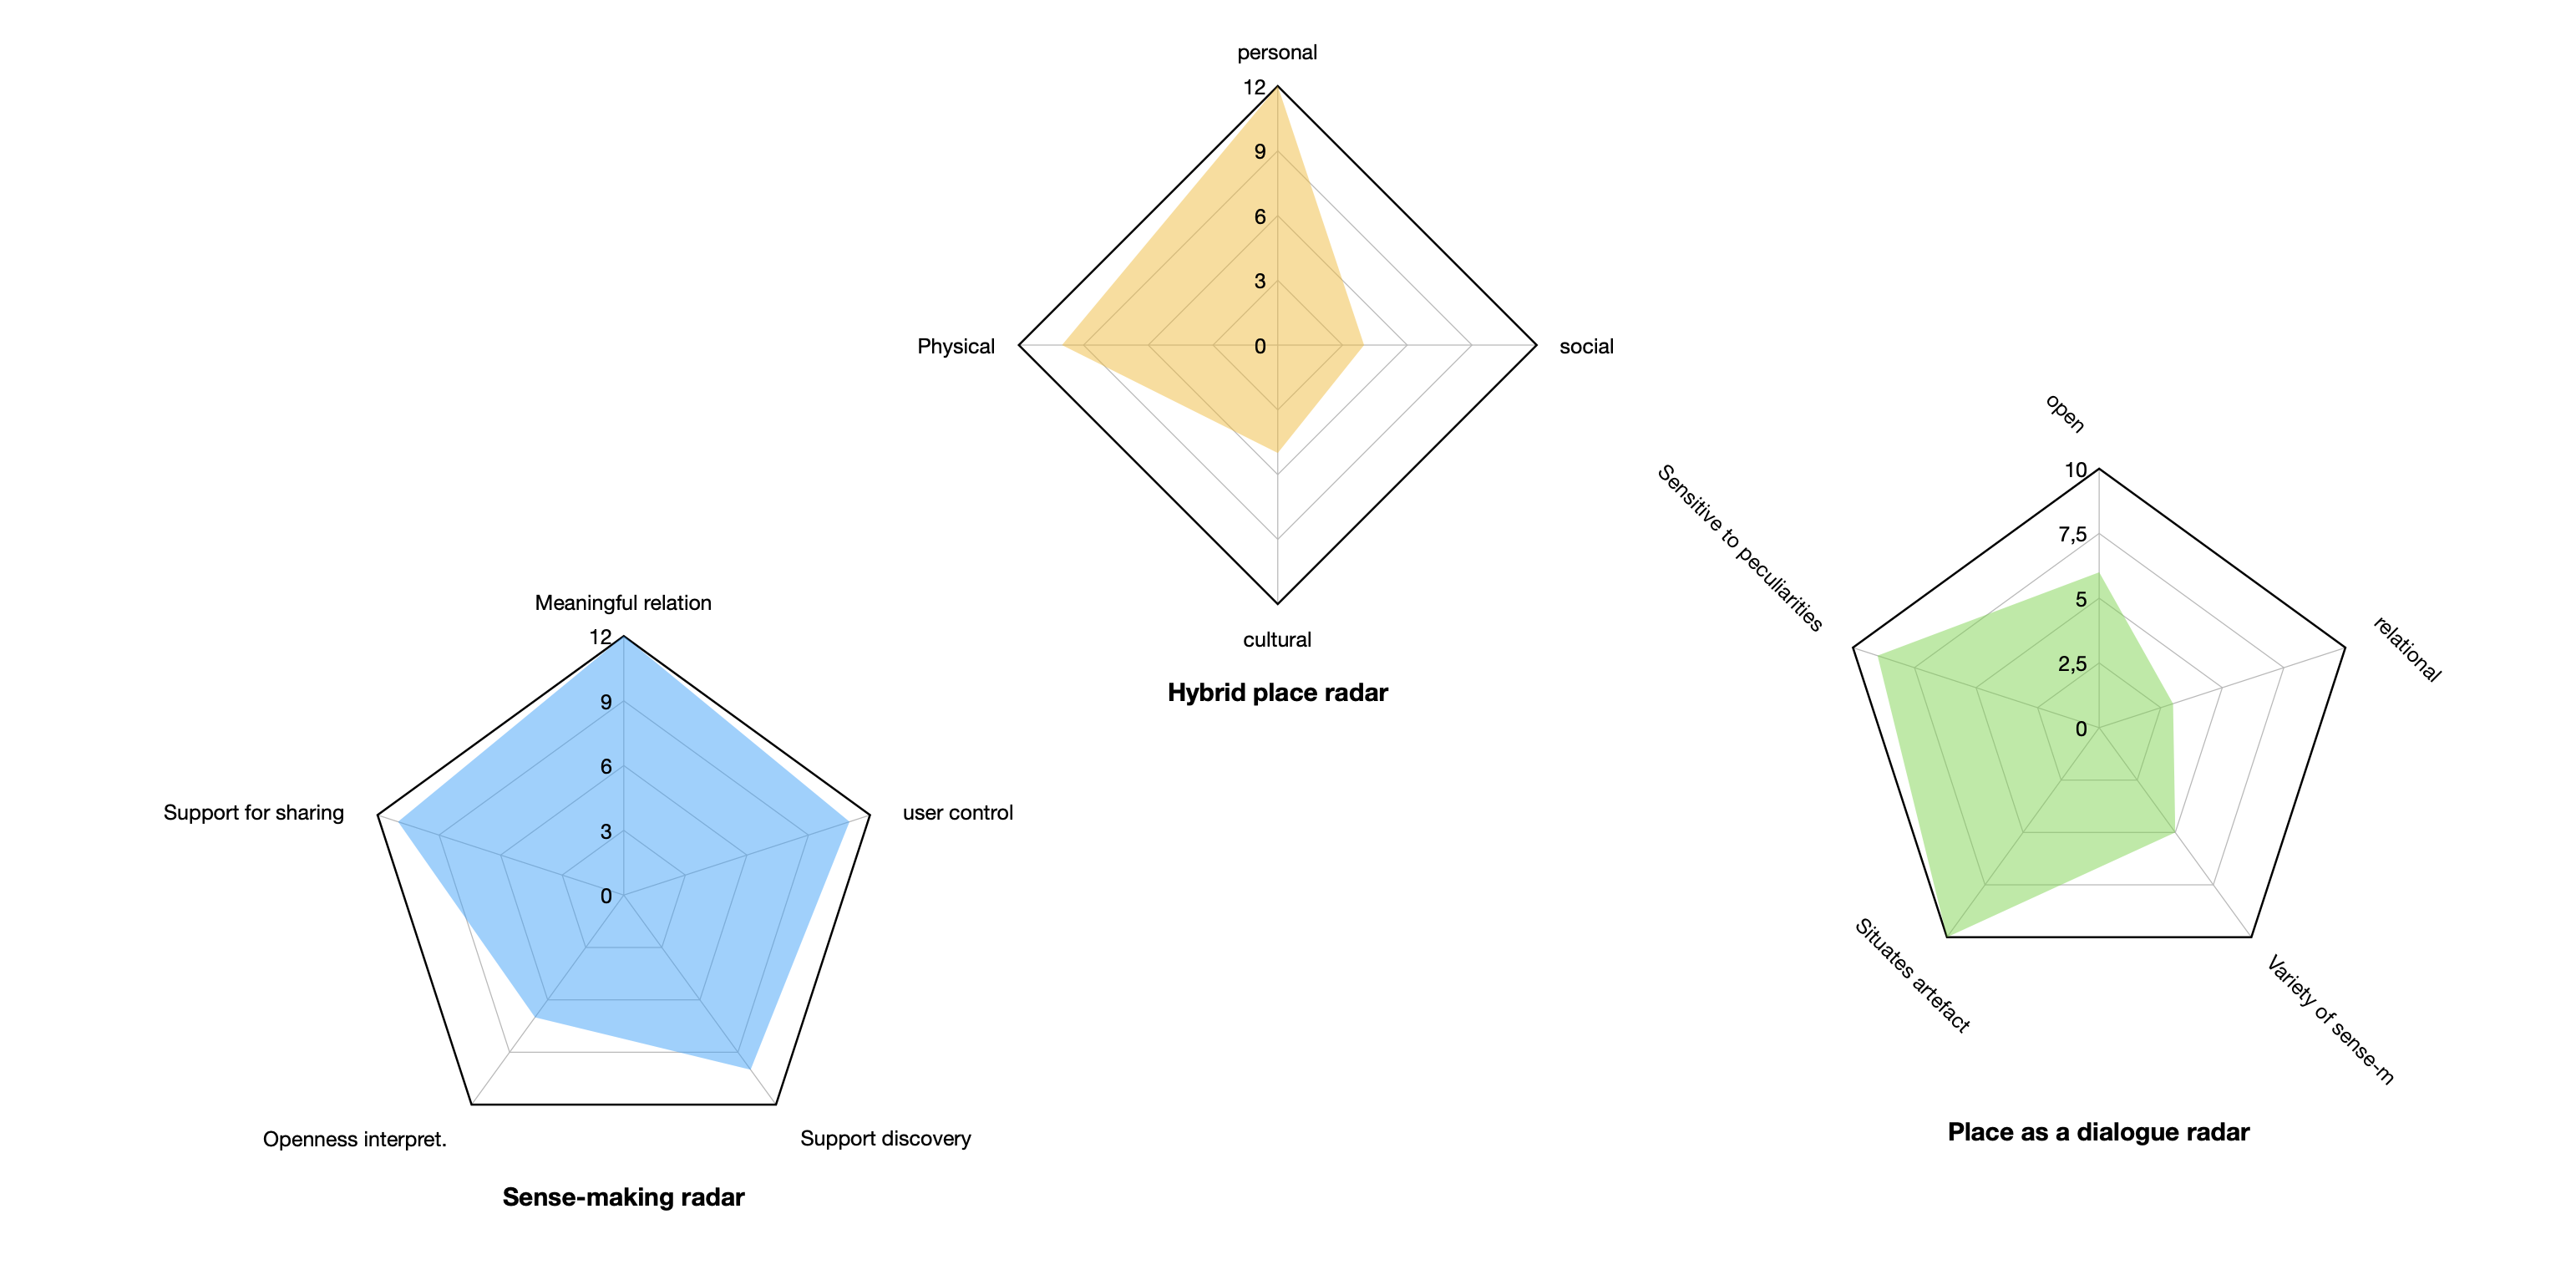
\includegraphics[width=13cm]{pictures/dataset/analysis_radars.png}
\centering 
\end{figure}

\emph{"Findings"}
\par

What I have learned by looking at the radar charts so far is how the different theories fulfill, or complement eachother. The way I have gone forward in looking at the radar charts is as following:
\par I'll start by looking at the hybrid place radar chart, noticing how the personal and physical dimension is fulfilled, while the social and cultural dimension is very little fulfilled. What does this mean? According to the Norwegian museum policy strategic thinking, it is wanted that museums transition from the personal dimension to the more social and cultural dimension. The fact that installations in my analysis shows presence in the physical dimension is positive, in terms of enabling the personal dimension, experience-wise, to involve more tangible or at least dynamic experiences in the museum space.
\par Then, if we shift focus for a second to look into the sense-making radar chart, we see that one of the corners that is fulfilled by almost all installations in this analysis - support for sharing is fulfilled. How come, that even though the social dimension is not fulfilled while almost all installations, in terms of sense-making have good support for sharing? 

\par Then again, we can look at what dialogic qualities the installations turns out to have little "relationalness", which is a dialogic principle/ quality that involves the Docents in the museum for example, or relational qualitites.






\section{Second iteration: looking for patterns}


\section{The role of prototyping in this thesis}
Research through design is a type of research practise where the researcher create artefact- or object prototypes to gain the necessary insight needed to drive and conduct the research project. Prototyping, or the use of prototypes can be used in a variety of ways, and in every stage throughout the project. In the field of human-computer interaction (HCI), software engineering and design, the term prototype is commonly used to signify a specific kind of object used in the design process (Lim et. al., 2008, p. 2). The prototypes are either physical or digital, and function as either a speculative solution, as a manifestation of a design idea, or to explore a design space - all in relation to the research scope and focus. Prototypes are the means by which designers organically and evolutionary learn, discover, generate and refine designs \cite{lim_anatomy_2008, p.2}. They are design-thinking enablers deeply embedded and immersed in design practise, not just as tools for evaluating or proving successes or failures of design outcomes (Lim et. al., 2008, p. 2).

In the search for a new way of thinking about prototypes and prototyping, based on the need for exploring and establishing a definition that differs from current approaches in software engineering contexts where engineers use prototypes to identify or satisfy requirements: Lim et. al., conceptualise prototypes as tools for traversing a design space where all possible design alternatives and their rationales can be explored (Lim et. al., 2008, p. 2). In that way, the prototype serves as a communicative manifestation, where the designer is enabled to communicate the rationales of their design decisions through the prototype (Lim et. al., 2008, p. 2). Prototypes stimulate reflections, and designers use them to frame, refine and discover possibilities in a design space (Lim et. al., 2008, p. 2). This new way of thinking about prototypes differs markedly from requirement-oriented approaches like software engineering, recognising design activities as flexible rather than rigid, reflective rather than prescriptive, and problem-setting rather than problem-solving (Schön, 1982). A design idea that satisfies all the identified requirements does not guarantee that it is the best design since a number of ways can meet each requirement (Lim et. al., 2008, p. 2). If the focus of prototyping is framing and exploring a design space, what matters is not identifying or satisfying requirements using prototypes but finding the manifestation that in its simplest form, filters the qualities in which designers are interested, without distorting the understanding of the whole (Lim et. al., 2008, p. 2). In order to support this perspective and to provide a stable foundation for the study of prototypes in HCI, Lim et. al. (2008) proposes a framework for conceptualising prototypes. The framework is an attempt to create an understanding of the nature of prototypes in general and to provide a language for articulating the characteristics of a particular prototype (Lim et. al., 2008, p. 3). Two fundamental aspects of prototyping form the basis of the framework:

1) prototypes are for traversing a design space, leading to the creation of meaningful knowledge about the final design as envisioned in the process of design, and
2) prototypes are purposefully formed manifestations of design ideas.
(Lim et. al., 2008, p. 3)

Will answer these:
What values are important in my context?
What is my design outcomes?
What is my design space?
Experience prototyping? Am I going to prototype an experience?
Why and how do I intend a particular prototype to support the design process?

In this thesis, the role of prototyping will be a proof of concept where the perspectives are manifested or represented. As a proof of concept of how I have used the framework/ thinking to design a meaningful interactive experience.
The prototypes main function is to work as a “mediator”, to facilitate for conversations with museumspeople or designer that will give insight to what the prototypes adresses.


\chapter{\ding{167} Design Process}

\section{Investigating narratives and storytelling with Klimahuset}
\par
\emph{31.05.2021, workshop with members of staff from Klimahuset}
\par

In the beginning of May 2021, me and my research buddies were requested to host a workshop for different members of staff from Klimahuset as a way to kickstart the collaboration with the museum. Inspired by readings on narrative theories and learning in contemporary art museums, and the way narratives are constructed in a museum context \autocite{narrative_sitzia}, we saw this as an opportunity to learn more about how narrative play a part in telling a story and in conveying a message. We wanted the workshop to explore how to engage participants in building a narrative, and anticipated that it would give us some insight on how to build climate-crisis related narratives. This would also give us the opportunity to get some input on which sustainability issues can be a better fit, topic-wise, when designing for a learning-oriented type of installation. Lastly, we wanted to facilitate a conversation on the current existing exhibition in Klimahuset, to get some feeling if there were any topics or sustainability issues they wished the current exhibition should address.

We designed the workshop timeline to endure three phases; brainstorming, storyboarding and presentation. Because of the ongoing pandemic we conducted the workshop digitally through Zoom, using Miro as the workshop platform-tool. We primarily wanted to get a better grip on different topics and issues in the climate debate that could be used as groundwork for design fictions, which is why we tried to brainstorm three dimensions that can make up a story; a theme, a dilemma and a setting. Therefore we asked them:

\begin{itemize}
    \item What topics in the climate debate do you think is important to address?
    \item Write down issues/ dilemmas related to climate debates.
    \item Write down (a climate-related) setting.
\end{itemize}

In the next part of the workshop we wanted the participants to create their own individual storyboard, where they could choose between all commonly brainstormed themes, dilemmas and settings - to make up their own story that they would later present. And then to finalise the workshop, the participants presented their own story. It was interesting to see the diversity and different perspectives from the participants and their respective stories. Even though some participants had used the same theme, dilemma or setting, they all differed in terms of what the participant wanted to convey with their story. 

In the aftermath of this workshop, the collected stories and notes from the discussions have worked as a foundation for me to look into the relationship between narratives, dissemination in museums and meaning-making. The main finding I got from the workshop is the notion on how a well written narrative have the power to make us think about or see ourselves and the Earth around us with new eyes, enabling us to engage in and relate to the climate crisis through the narrative that is told. The climate crisis is first and foremost a story about humans and humanity, and the power in the narrative therefore lies in the message conveyed. 

\begin{figure}[h]
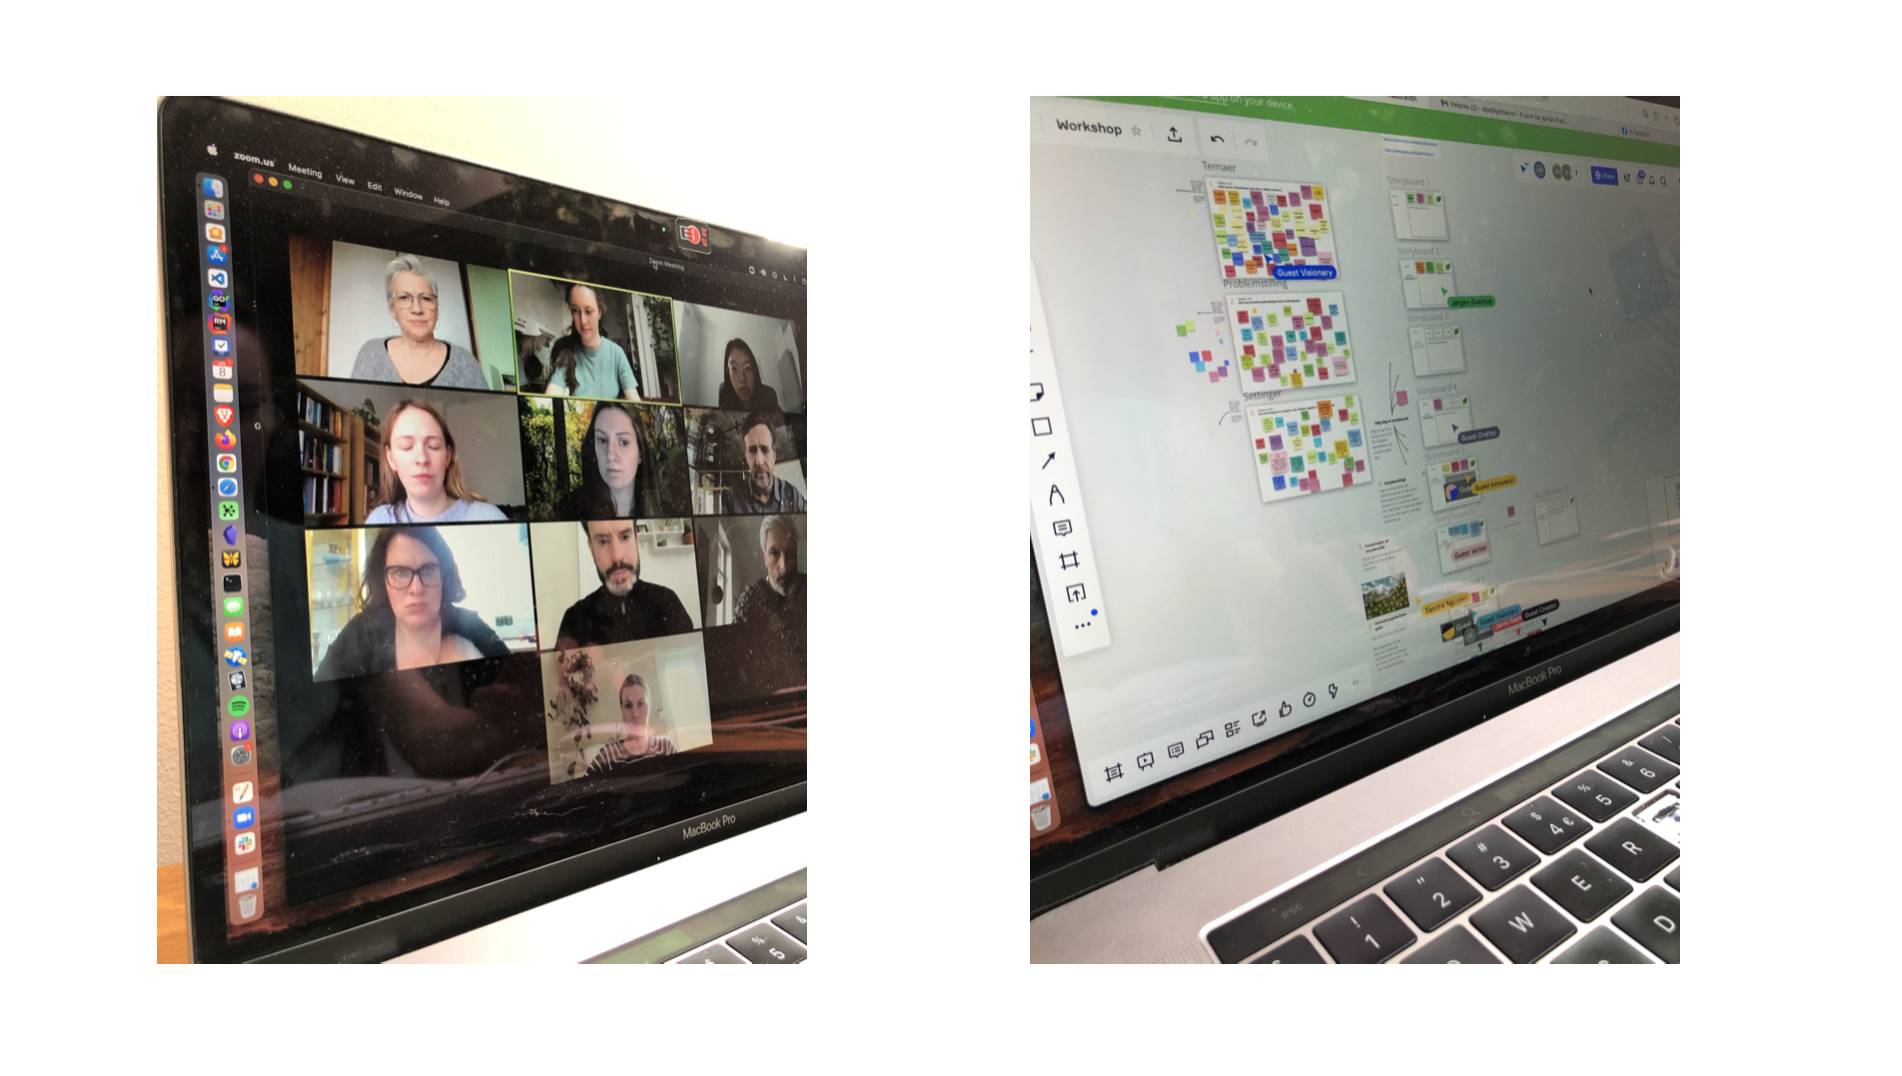
\includegraphics[width=13cm]{pictures/narrative_workshop.png}
\centering 
\end{figure}


TODO: Add workshop guide in appendix, and elaborate more on the actual workshop design. Account for the choice behind the workshop design, and be more clear about what the RQ and research motivation at the time was. And also what lessons learned I/we had, and how that affected the way forward.


\section{Exploring input through plants}
\par
\emph{01.05.2021, presentation at Klimahuset}
\par

The thought behind this project was to explore how human touch on plants could be used as input, or as a type of controller, to manipulate elements of the installation. The statement of using an actual, living plant would be a direct reference to the relationship between human and nature: plants, animals and ecosystems, bringing nature closer to the discourse where sustainability issues are discussed, inviting to reflections to the ecological damage that we are responsible for. I think this exploration addresses the research question as to how interactive artefacts can provide new depth to the museum discourse, by exploring how human touch through plants can stimulate emotions or values like empathy and awareness, reinforced by the educational environment (the whole museum) the installation is placed in. I believe the plant installation could be interesting to use in combination with learning about plant/ nature related climate disturbances like the burning and destroying of the rainforest, but also in a local, Norwegian context; the windmill debate, hydropower, national park borders, repercussions of cottage development or light pollution. During the shaping of this exploration, I managed to define yet a research question that I want to inquire into; can new/different interactions with natural objects contribute to increased climate consciousness and activism?	

\begin{figure}[H]
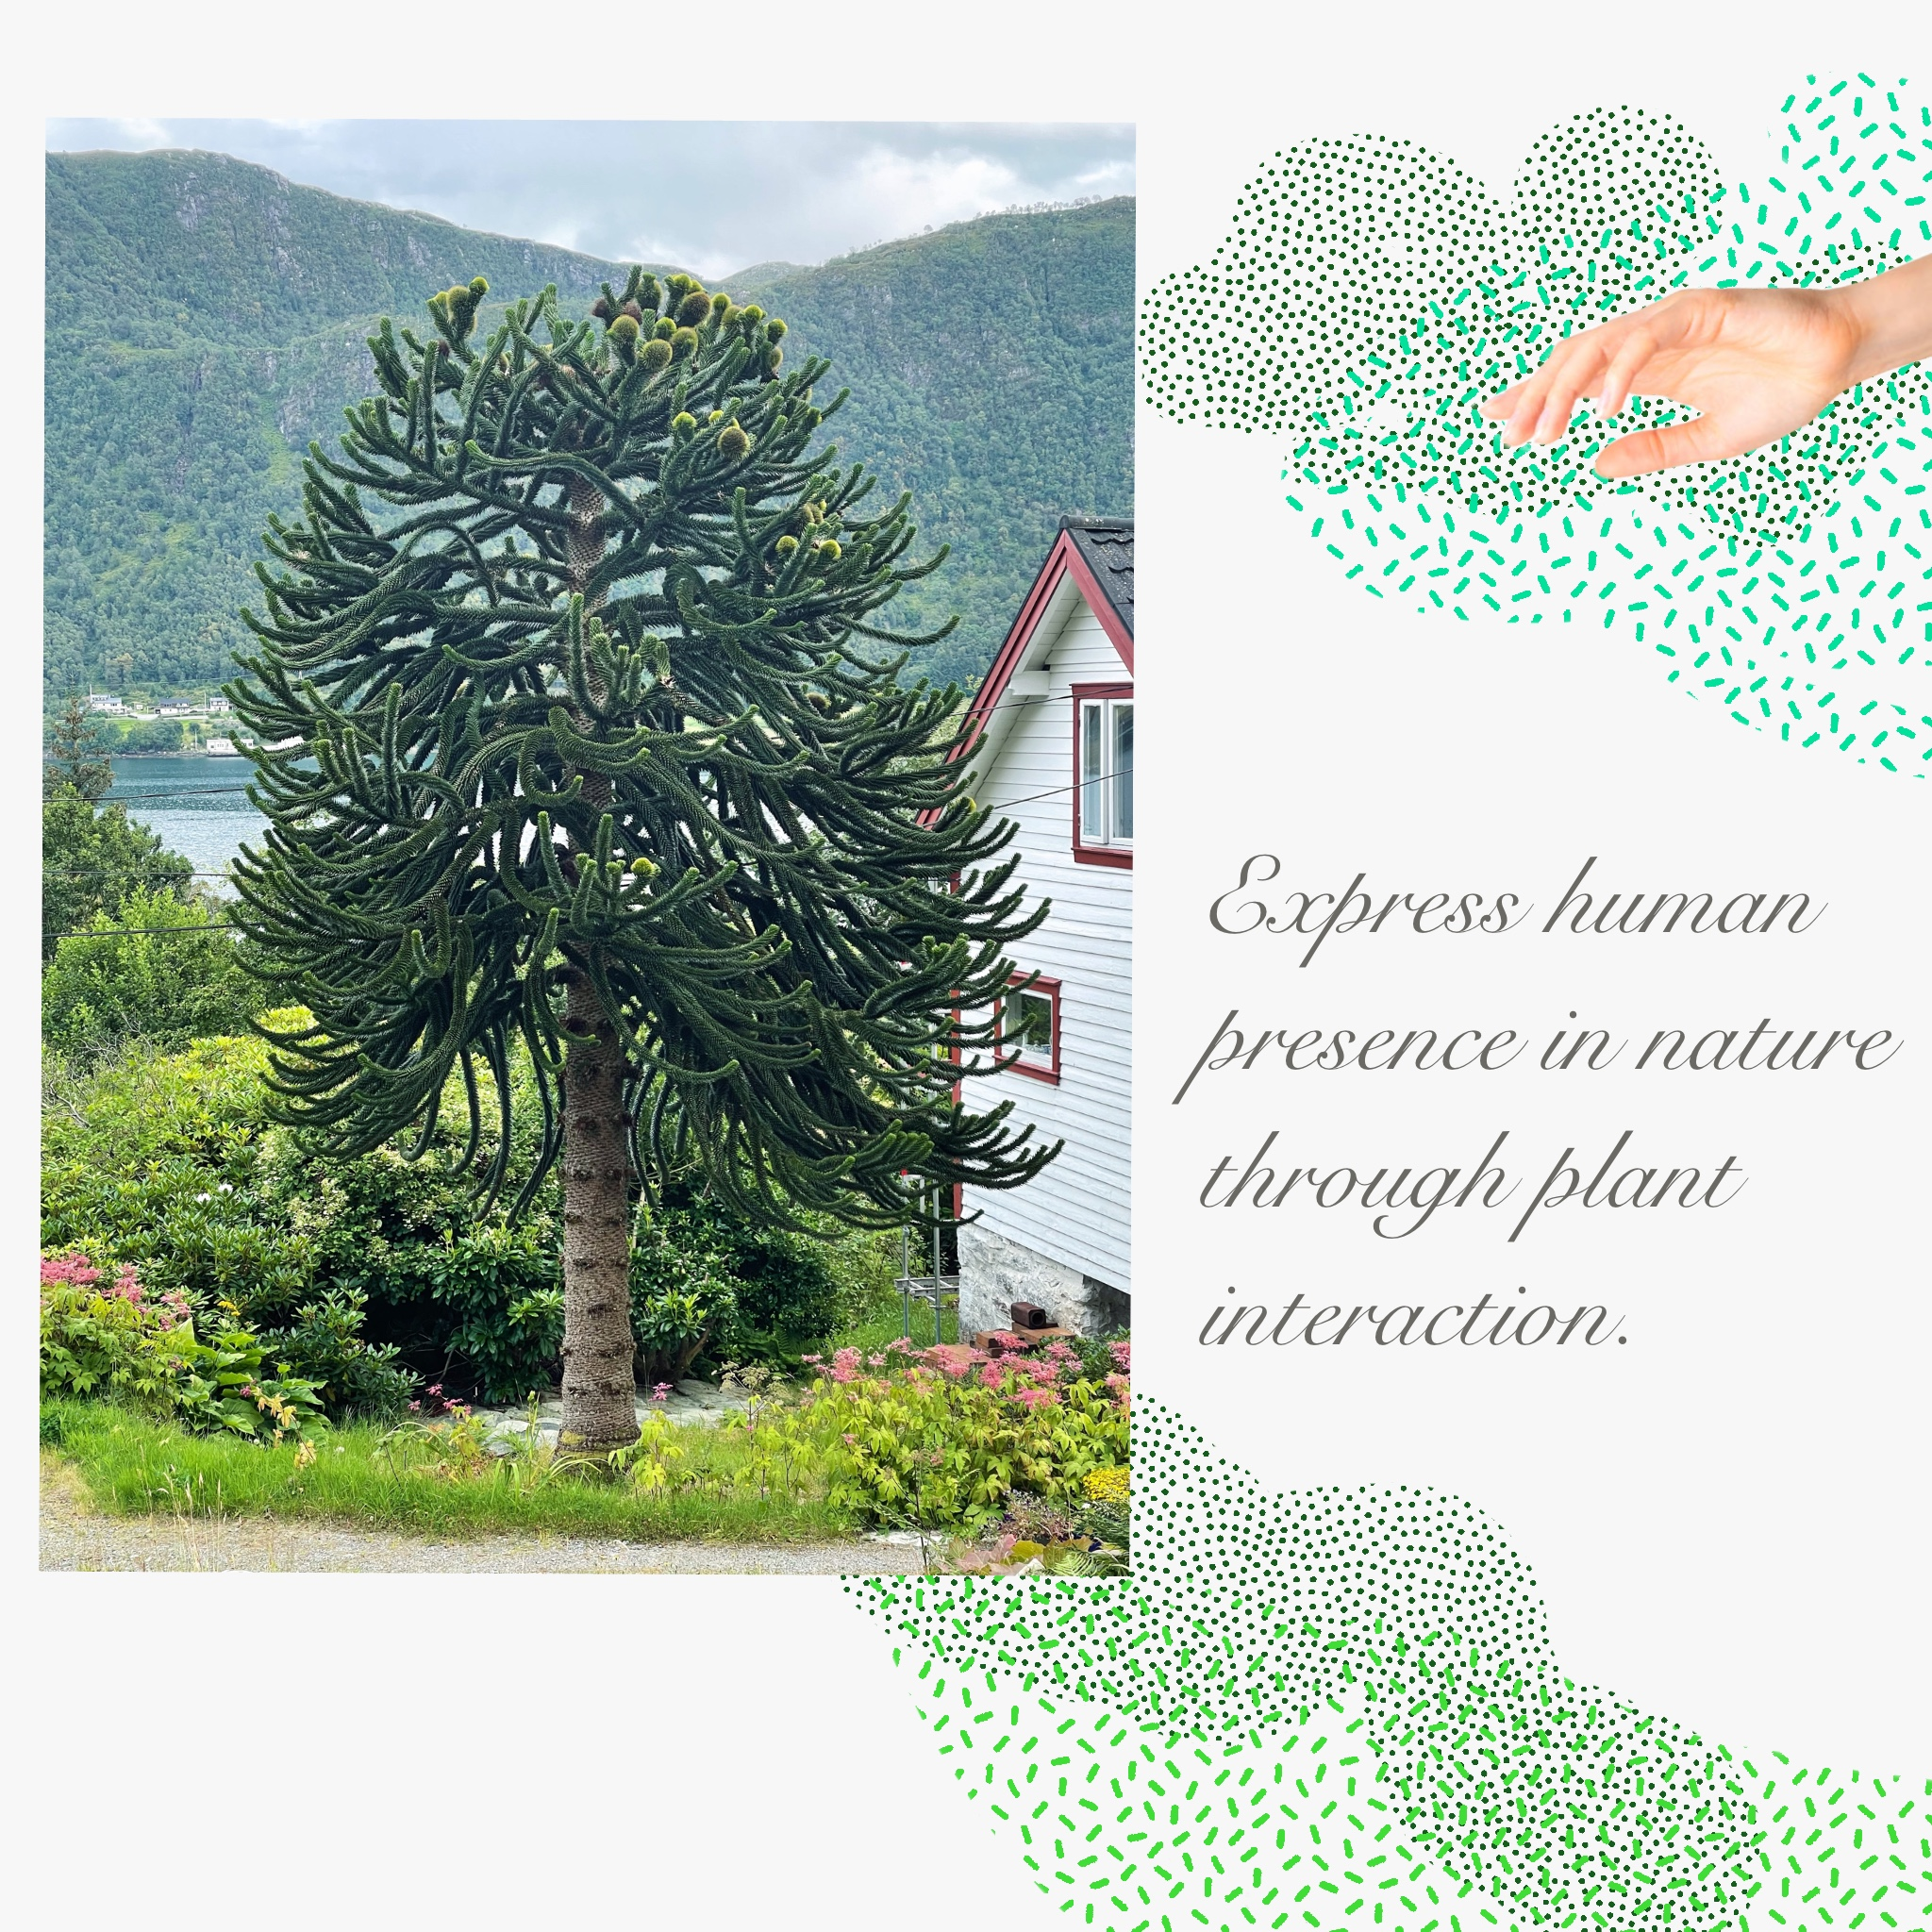
\includegraphics[width=13cm]{pictures/human_presence.jpg}
\centering 
\end{figure}


\section{I/O (In Oslo) by Yuko Mohri}
\par
\emph{22.10.2021, excursion to Atelier Nord}
\par

In late October, me and my research buddies visited Atelier Nord to see and analyse the ongoing exhibition by Yuko Mohri: I/O (In Oslo). Going in, we expected the exhibition to be or have interactive qualities, and my research interest during this fieldwork was guided by \autocite{hybridplace_ciolfi}'s Hybrid Place dimensions. 

This is how Atelier Nord describes the installation: 
\emph{Gently cascading rolls of paper are fixed to a framed structure in the ceiling and pick up dust and other debris. The traces are scanned and converted into random input-output signals that case a constellation of objects, such as feather dusters and old musical instruments, to move and produce sound. The site-specific characteristics - including movements of air, humidity, and the undulating surface of the floor - are picked up by the rolls of paper, gradually permeating it with the unique features of the exhibition space. The result is an organic environment where the same sound and movement never occurs twice. In this case, the gallery might be likened to a biotope-like ecosystem that interweaves the natural and artificial.} \autocite{yukomohri_web}

Guided by the Hybrid Place framework, I first looked for the physical and structural qualities of the space. I noted how the showroom was large, kind of empty and very open. The installation itself consisted of two separate installations, both placed in the center of the room, so that visitors could walk both around and in-between the two installations. There was also a small room where the visitor could see a movie about Yuko Mohri and her thoughts behind the installation. There was no tape on the floor, or signs saying to not touch or walk, and in that sense the showroom invited to make our own path and discover the installation in our own pace and way we wanted. The showroom was pretty small, perhaps around 30kvm, and aesthetically quite plain. The wooden floor creaked when walking, and the sound echoed through the space. There was no music or what-so-ever in the background, only faint city-noises from one side of the housing and rustling of leaves from the other. The installation produced sound randomly from two outputs; feather dusters and an old musical instrument. During our visit we only heard the thumping from the feather dusters you can see depicted above. I noted how "clacking" sounds from both my own and other visitors shoes directed the attention toward movement in the room. The effect were especially reinforced after standing still for a while, looking, thinking about the installation. I noted that in the moment, sound and movement produced by the other visitors in the room influenced my mental presence being drawn back-and-forth, in-and-out, from the mind-space I was present in when observing and thinking about the installation, and then drawn back again to the physical space. Because of the showrooms atmosphere as I just described, and the room being small, it's easier to meet eye-to-eye with the other visitors, listen in on their conversations, and simply being aware of their presence. It felt a little awkward to talk, and sometimes also to move, resulting in a quiet/ whispering way of communicating with my research buddies during the visit.

\begin{figure}[h]
    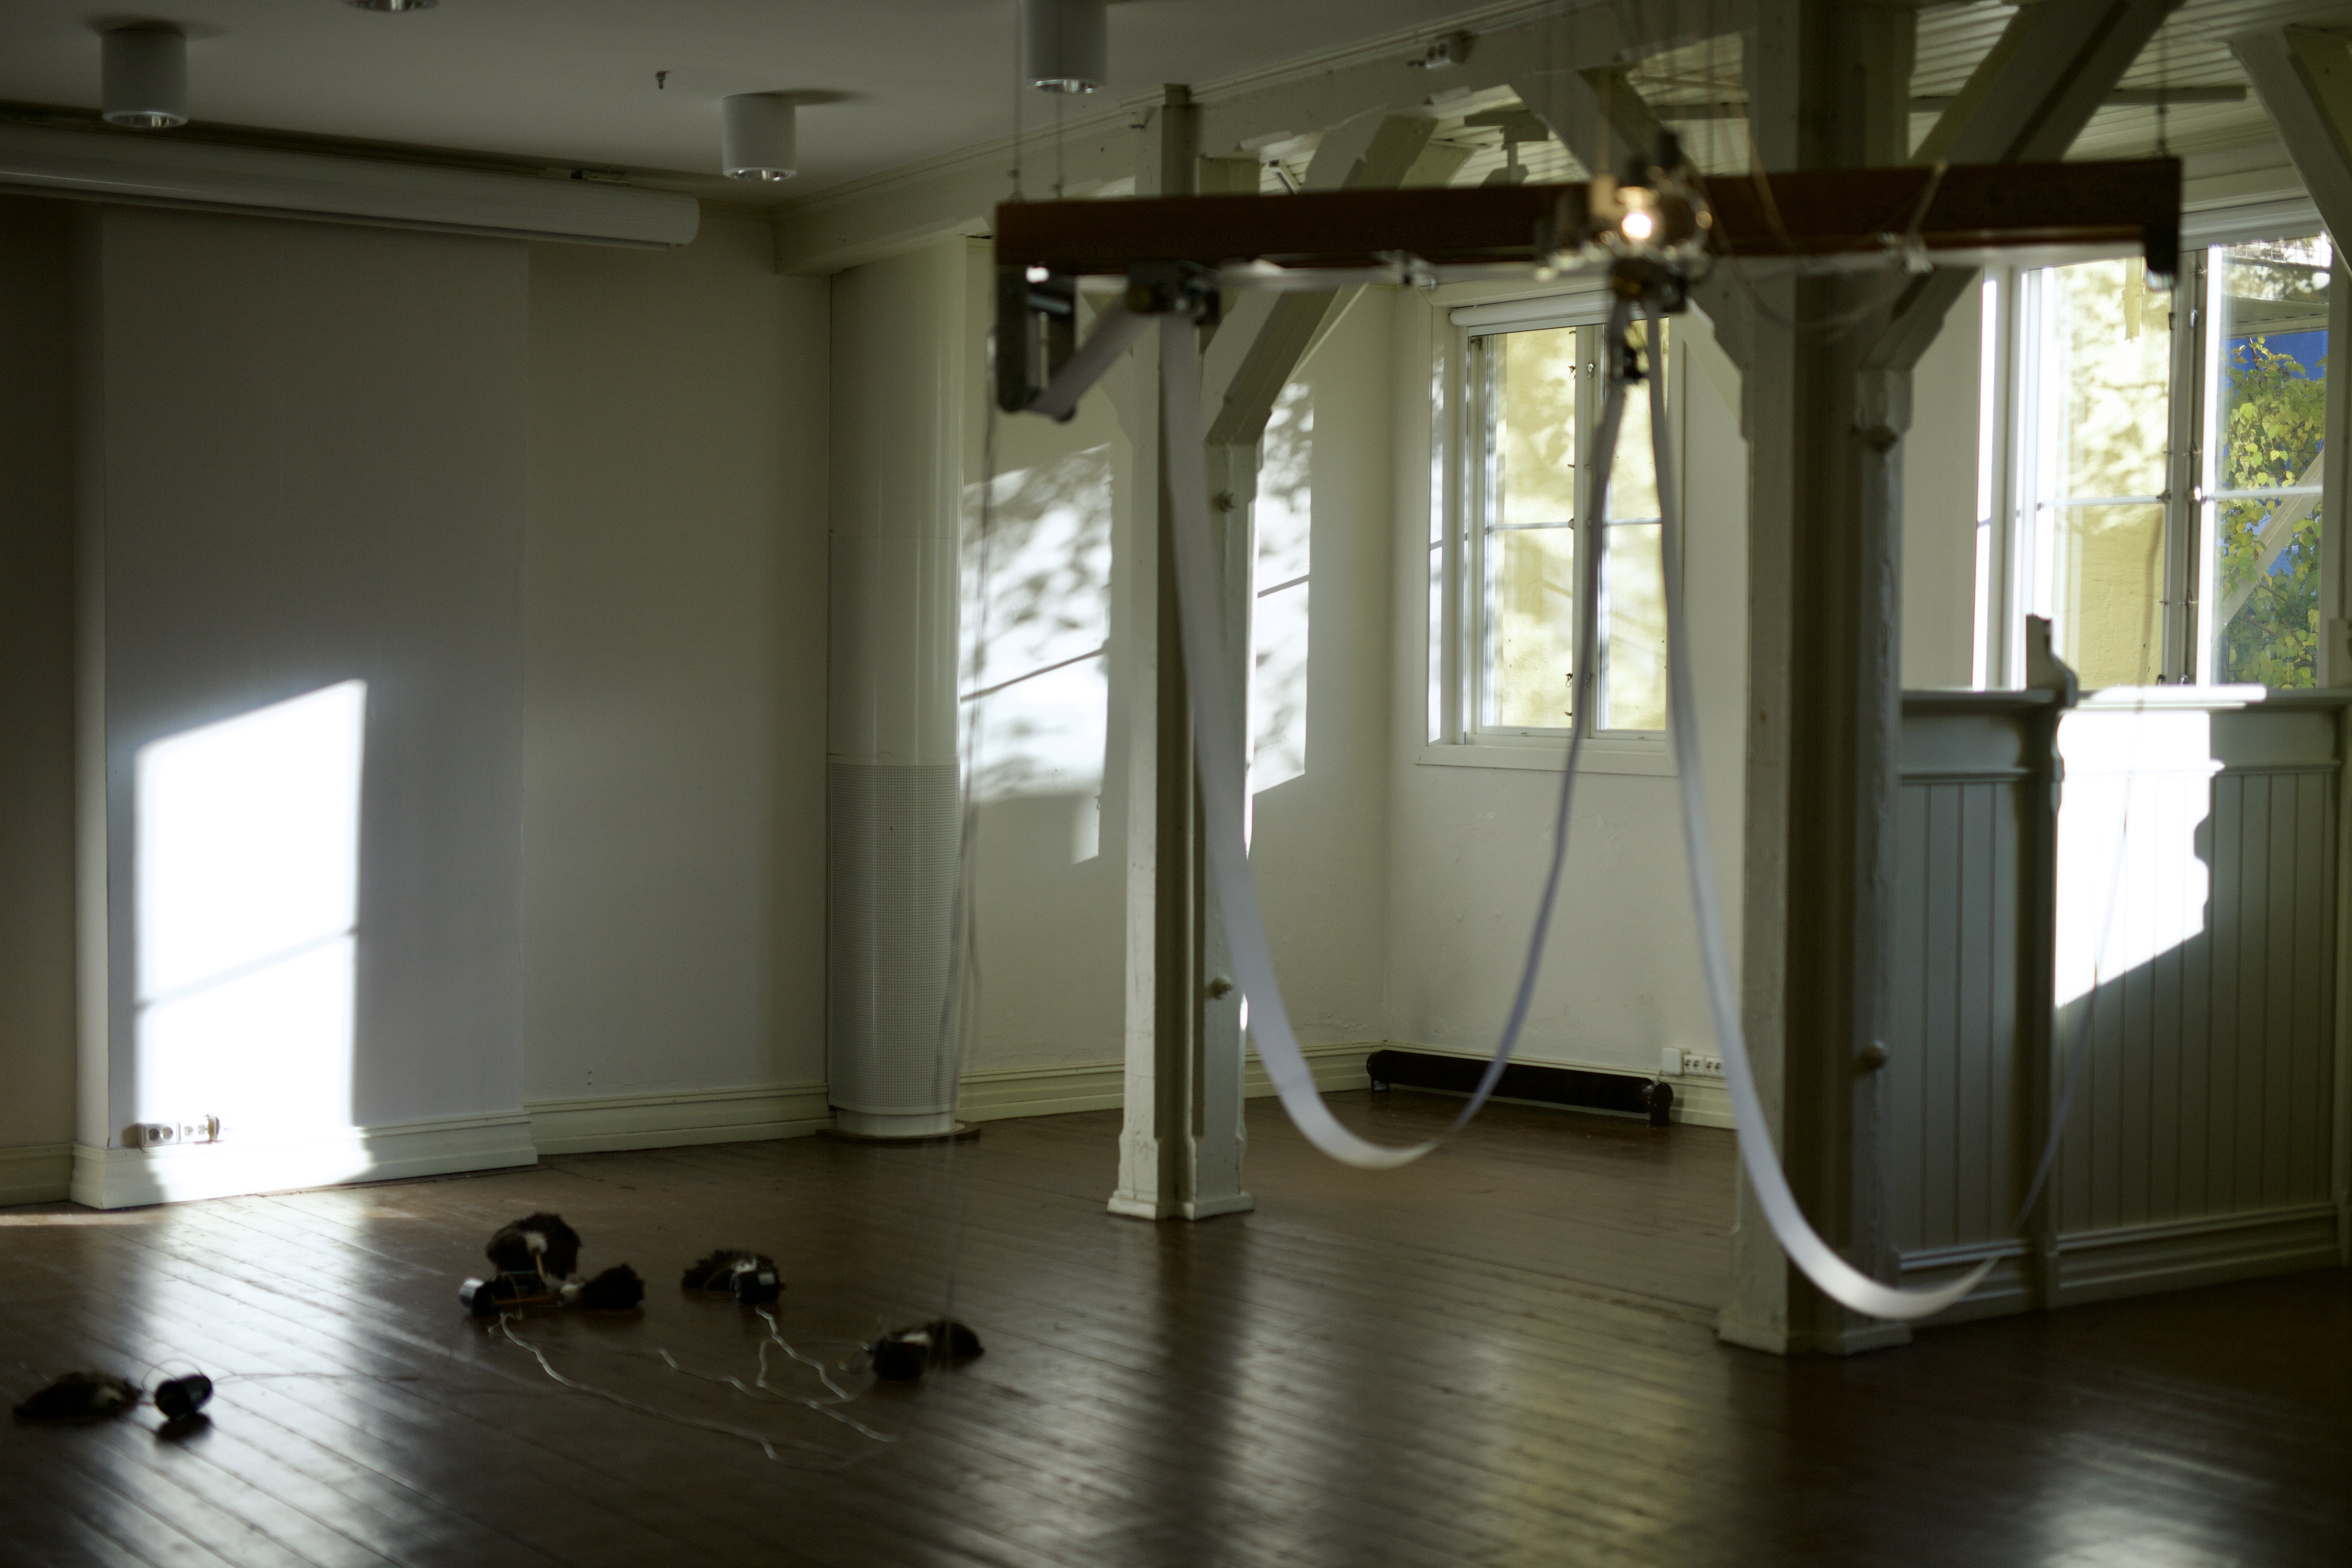
\includegraphics[width=12cm]{pictures/process/yuko_harmony.jpeg}
    \centering 
    \caption{Notice how the sunlight add a layered meaning to traces in the air being picked up by the cascading rolls of paper.}
\end{figure}

In terms of the physical/ structural dimension \autocite{hybridplace_ciolfi}, I would say that the space support group interactions, but it doesn't favour it. At least not in my experience. Therefore, I noted that the exhibition did not fit into the social dimension of the Hybrid Place framework. Coming into the showroom in a group of three, we actually had the space to ourselves for quite some time, but we walked around in silence for most of that time. Eventually, two people entered, and we were then not alone. Because we already had been there a while, we shifted focus from the installation to see how the pair moved around and used the space. The presence of a new group of people did not change the atmosphere as I described, they were also walking slowly, talking in a quiet manner and payed attention to the way we moved around the installation as well. I actually did not notice the video-room before these two new people entered, and went into the movie room as one of the first things they did after orienting themselves on the space. 

+ personal
+ cultural


\begin{figure}[H]
\includegraphics[width=12cm]{pictures/process/yuko_presence.jpeg}
\centering 
\end{figure}

The Docent who was in charge of the space and exhibition was quiet, looked tired, and did not initiate any dialogue or conversation about the installation. We were kind of just left to ourselves the entire time.


\begin{figure}[H]
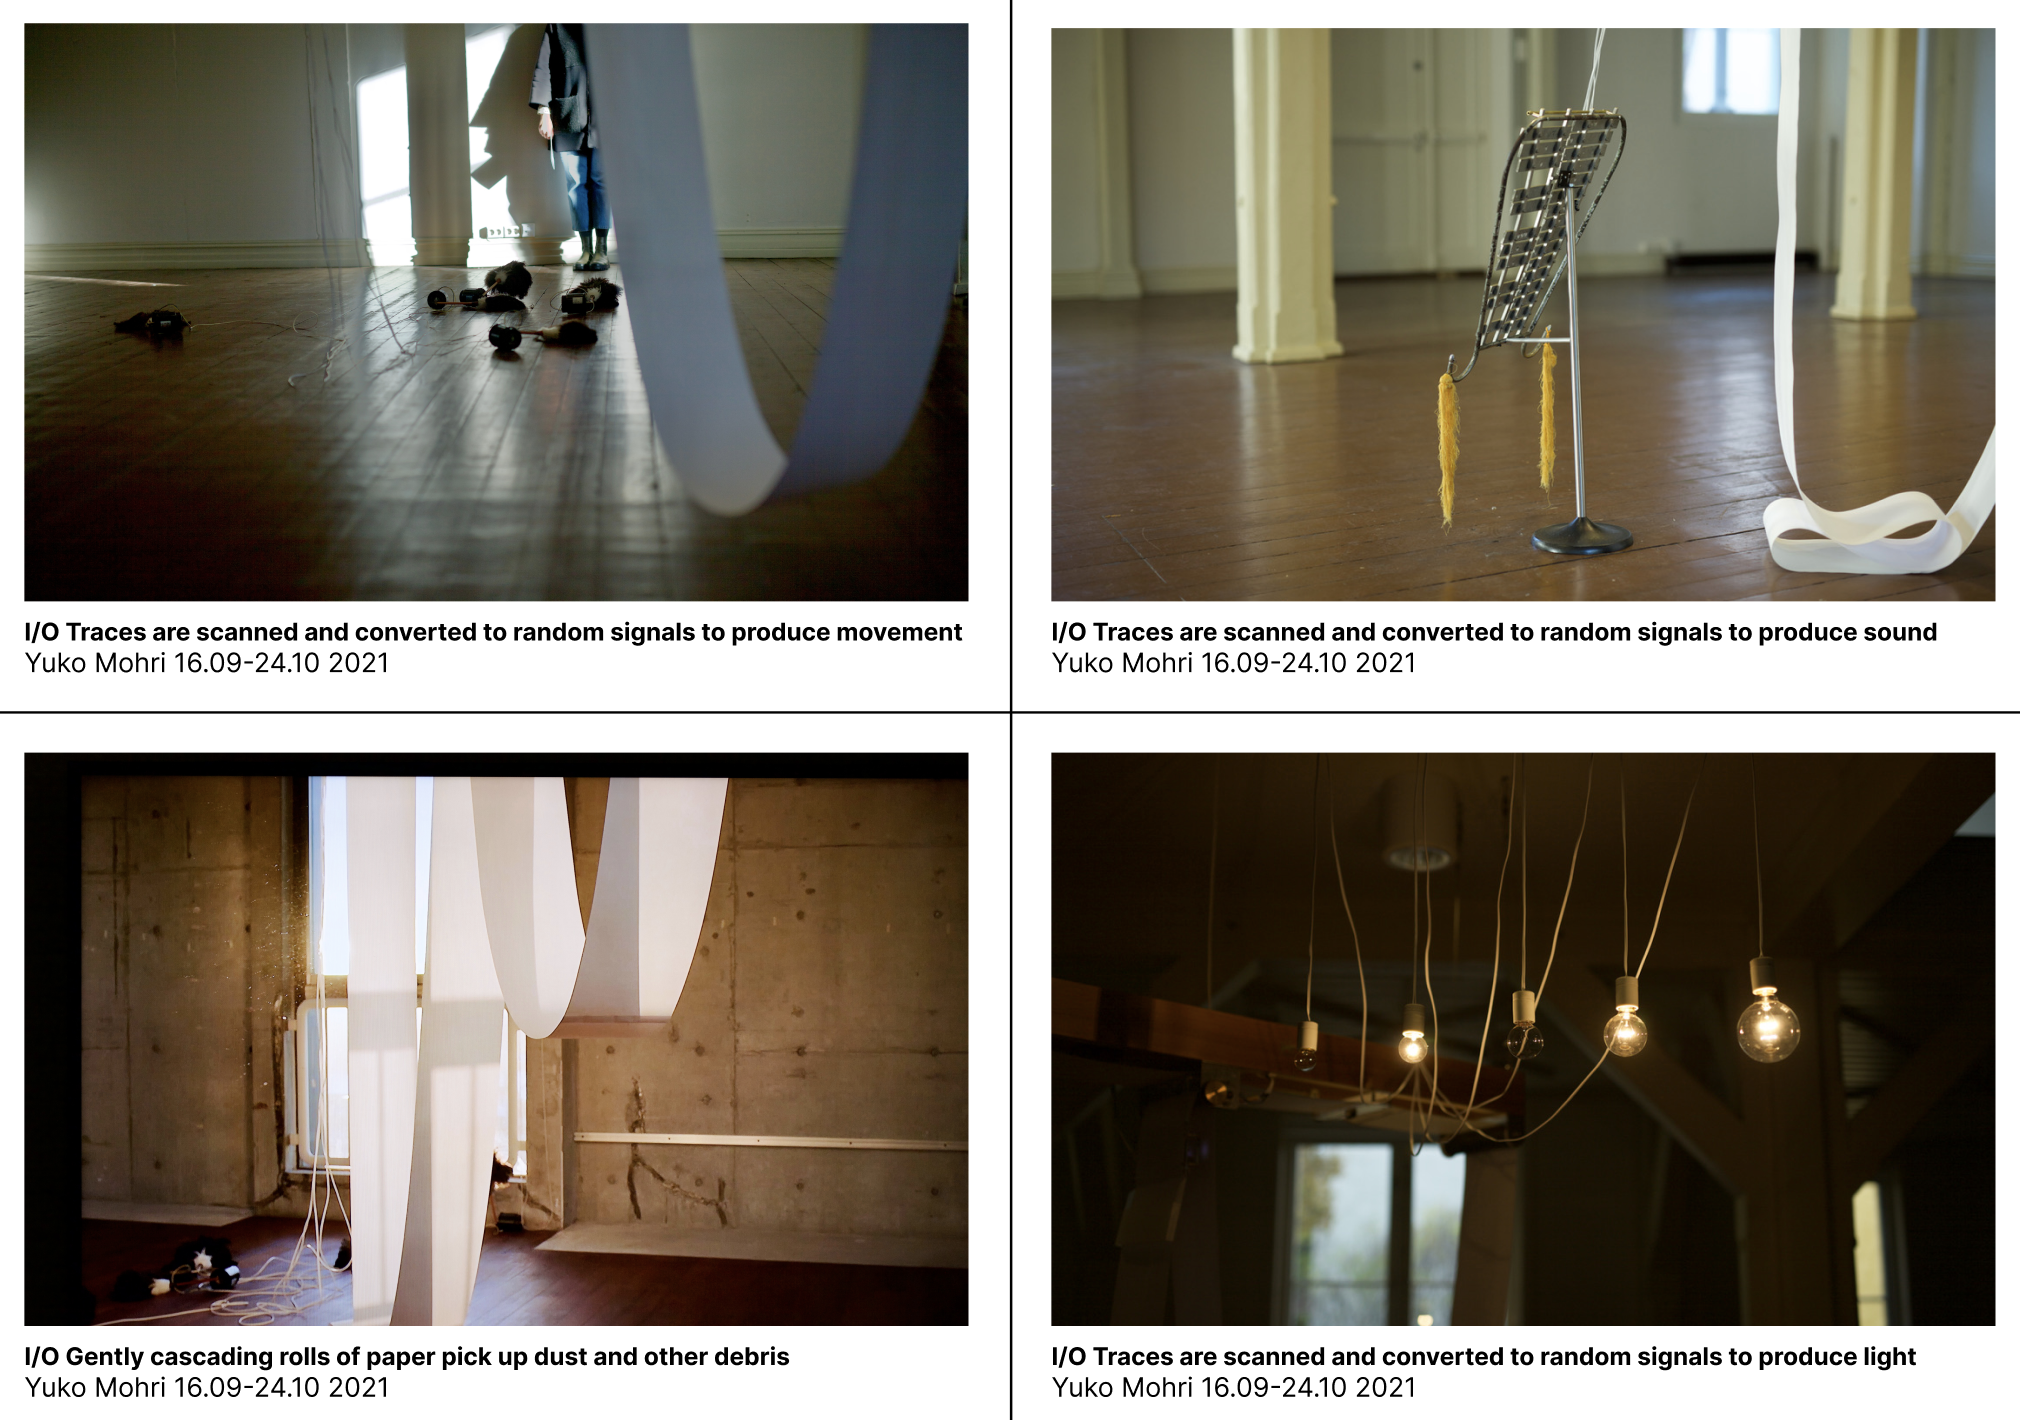
\includegraphics[width=12cm]{pictures/dataset/yuko_mohri.png}
\centering 
\end{figure}


\section{Poison by Munch}
\par
\emph{27.10.2021, excursion to Munch Museum w/ focus on the temporary exhibition Poison}
\par

Munch is a great example of how they use text and plaques to inform/guide the visitor in terms of how they can read some of the art they see. It is a good example of how one can design the visitor journey through the exhibition space. It supports the visitors sense-making, in terms of how they can use and move through the space. However, it is an analogous way to support sense-making, while I am interested in ways interactivity can support this type of sense-making. Even in the interactive Poison exhibition, the information is static.

\begin{figure}[h]
\includegraphics[width=12cm]{pictures/process/pink_munch.jpeg}
\centering 
\end{figure}

\section{Qi by Qi}
\emph{date xxxx, invited to host an energy-visualisation workshop}
\begin{figure}[h]
\includegraphics[width=11cm]{pictures/dataset/Qi.pdf}
\centering 
\end{figure}

\section{Slow Design and Haptic Interaction by tangible interaction students}
\par
\emph{date xxxx, what is it}


\section{Observing Klimahusets narrative storytelling in-action}
\par
\emph{Observation and interview 16.02.2022}
\par

After my readings on the museum and its expository agency, I wonder what Klimahuset’s stakeholders thoughts are on their agency? And their position toward whether or not they have a subjective or objective expository agency? What are the cultural attitudes, decisions, views and stances the agents involved in designing the climate exhibition in Klimahuset, took before they decided to do the act of exposing? What cultural function does the objects on display in Klimahuset pose? 

Some of these questions can already kind of be elaborated for, from initial reading on internal documents that I have gotten access through collaborating partners in Klimahuset, as well as from conversations with stakeholders from Klimahuset last semester through the workshop, mail correspondence and mini-exhibition. As accounted for in Klimahusets founding documents, their vision/ purpose of the museum is as follows:
To give the visitors an understanding of the most important climate processes that affect the living conditions on Earth so that they are able to develop their own views on climate change, take part in climate discussions or act in other ways in relation to the topic.
Visitors must gain an understanding that natural conditions also affect social structures and culture.
	
Building on Mieke Bal’s narrative analysis on cultural imperialism in museums, say we look at Klimahuset as an ethnographic museum with the expository agency to display installations, objects and data related to the climate crisis. And with a distinct and clear target group being children aged 10-14. Is Klimahusets agency and vision an attempt to display the climate crisis as a current/ ongoing discourse with the function to educate and stimulate critical reflections on current societal norms and ways of living, or is the agency to define and lay up cultural change, to a more sustainable way of living? Maybe both? If so, then comes the question if the museums cultural stakeholders, with this expository agency, are they cultural moralists? Especially because their whole museum exhibition are designed to engage children aged 10-14, though welcoming all age groups, raises the question if the museum and exhibition design in itself potentially have any moral imperialistic function as well, as to who the discourse (the climate crisis) is relevant for. 
Asked the klimaverter about  this, need to do some structural analysis of some sort….

\begin{figure}[h]
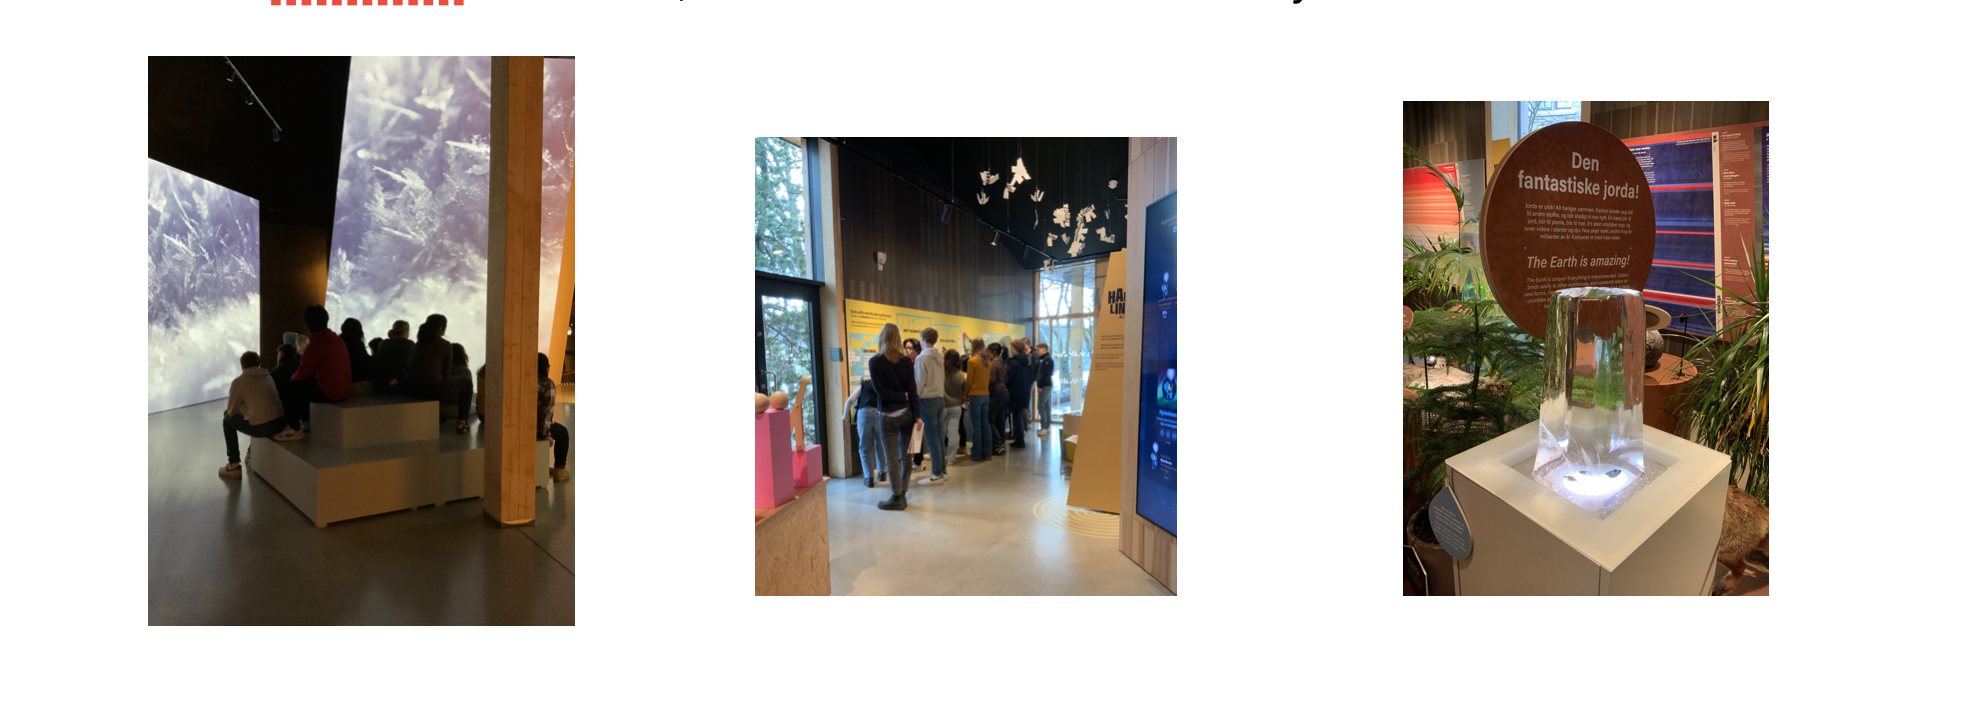
\includegraphics[width=13cm]{pictures/elever_i_klimahuset.png}
\centering 
\end{figure}

Med en klimavert til stede får man bedre hjelp og en form for retning til å “lese” installasjonene, som støtter deg når du senere går gjennom avdeling for avdeling. 
Man blir stilt spørsmål som er knyttet til faktiske ting, som for eksempel i video-atriet sier klimavert; jeg er 160cm høy, hvor høy tror dere denne veggen er?
Etter litt håndsopprekning får vi vite at dersom Grønlandsisen smelter vil havet stige like høyt som det den veggen er. Det er tankevekkende og setter inntrykk!

Her blir man også litt senere spurt: ser dere vær eller klima? et åpent spørsmål som setter i gang en god diskusjon på forskjellen mellom vær og klima, med fokus på hvordan vær påvirker klima. Dette blir forklart at mange blander og tenker at vær og klima er det samme, og at klimaforandringer og værforandringer ikke er det samme. Her får noen elever aha-øyeblikk.


Et annet eksempel er isbiten inne i “den naturlige avdelingen”.  Først får elevene i oppgave å finne noe i området som påvirker klimaet naturlig. Senere når det blir tatt en liten runde spør verten; har alle tatt på isbiten? For så å gå videre til å forklare hvordan menneskelig påvirkning påvirker klimaet. “For eksempel har deres varme hender bidratt til å smelte litt av isbiten her i Klimahuset”. Dette er også tankevekkende og setter inntrykk!


Ice Cube: a good example of a meaningful exp. !!!


\section{Interview with a concept developer from Munch}
\par
\emph{date date date}
\par





\part{Review/ Evaluation }

\chapter{\ding{167} Analysis}

\section{Narrative workshop dataset}



\section{Museum visit dataset}

Over the course of this thesis, my research buddies and I have visited in total 10 exhibitions from 7 different museums in Oslo. From these museum visits, we have documented 22 interactive installations that forms the dataset used for analysis and similar investigations in our respective thesis's. 

\begin{figure}[H]
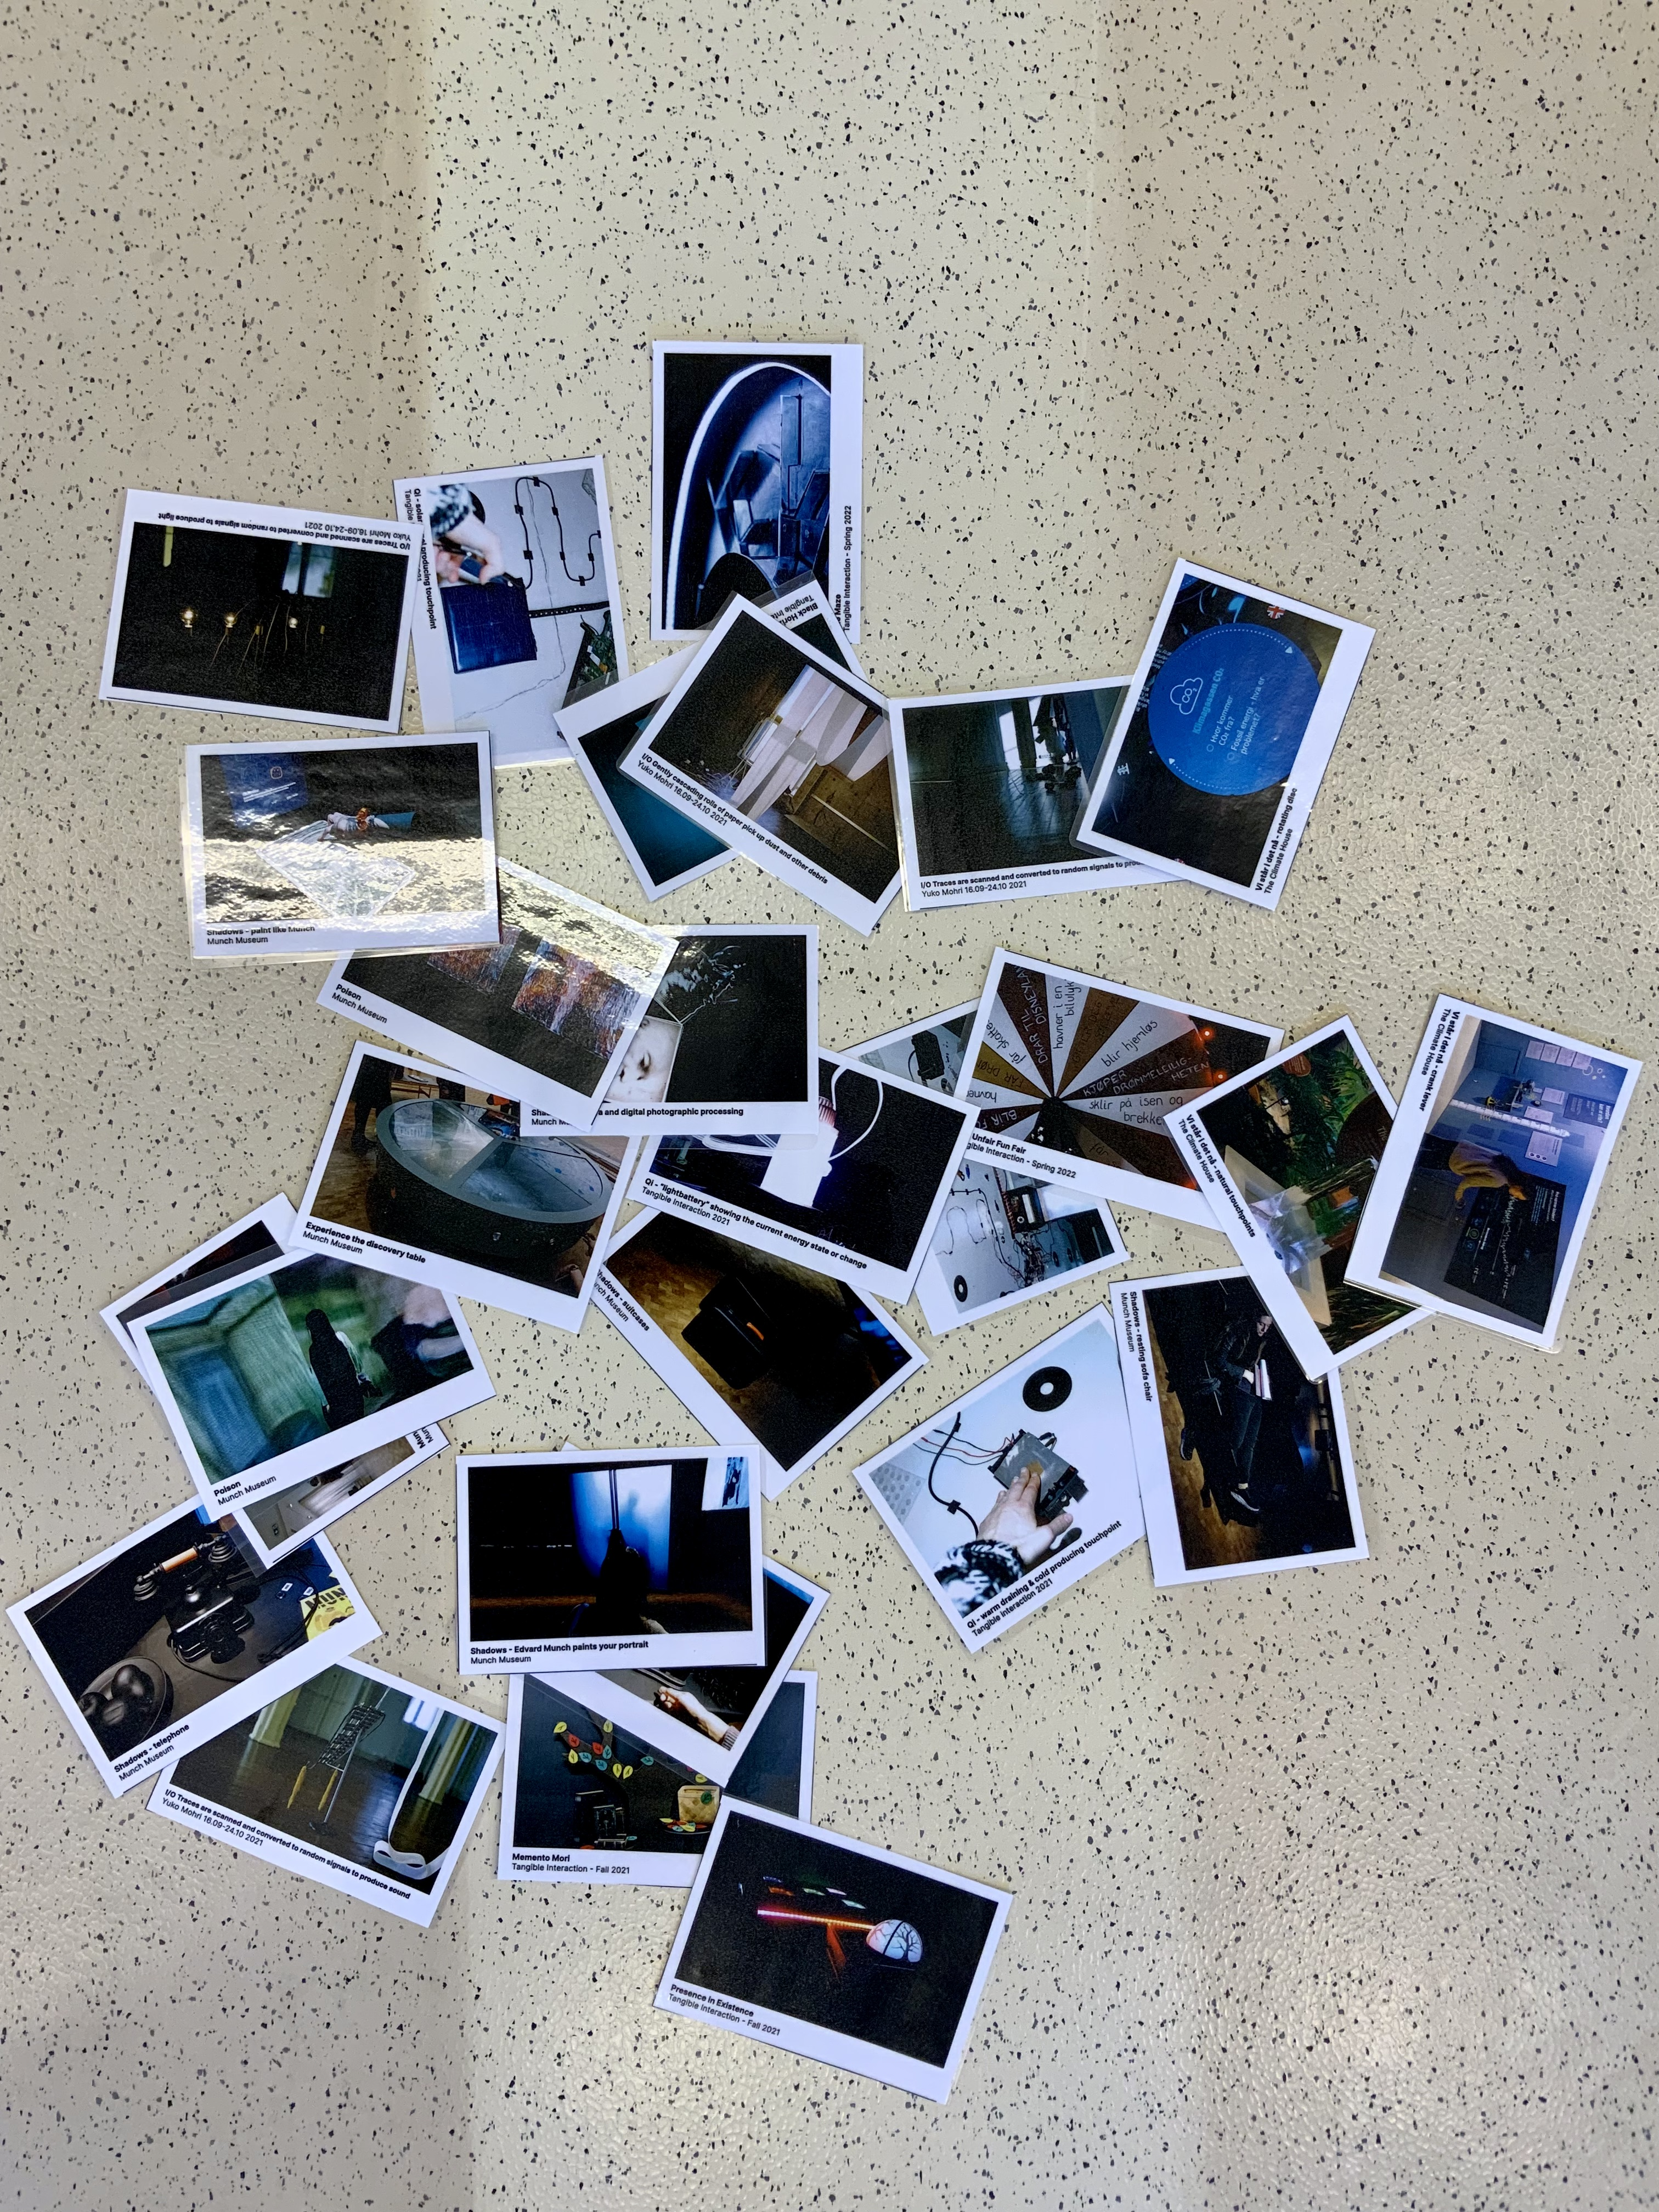
\includegraphics[width=12cm]{pictures/dataset/datasett_oversikt.jpeg}
\centering 
\end{figure}

I think this is basic qualitative analysis?

Måten jeg har gått frem på ved bruk av dette datasettet, sett opp mot mine utvalgte teorier, har vært en form for deduktiv systematisk prosess. Det vil si at jeg til å begynne med har systematisert og kategorisert installasjonene opp mot hver teori; feks som jeg har gjort her fra en av de interaktive installasjonene på klimahuset haar jeg

\subsection{"data laundering"}
Write out:
\begin{itemize}
    \item explain why munch shadows is analysed as one. and only weighted as one. and how that affects the dataset.
    \item discuss how the amount of tangible installations affect the dataset
    \item discuss the analog-tangible vs interactive-tangible installations (ice cube, munch peepholes and discovery table)
\end{itemize}

\begin{figure}[H]
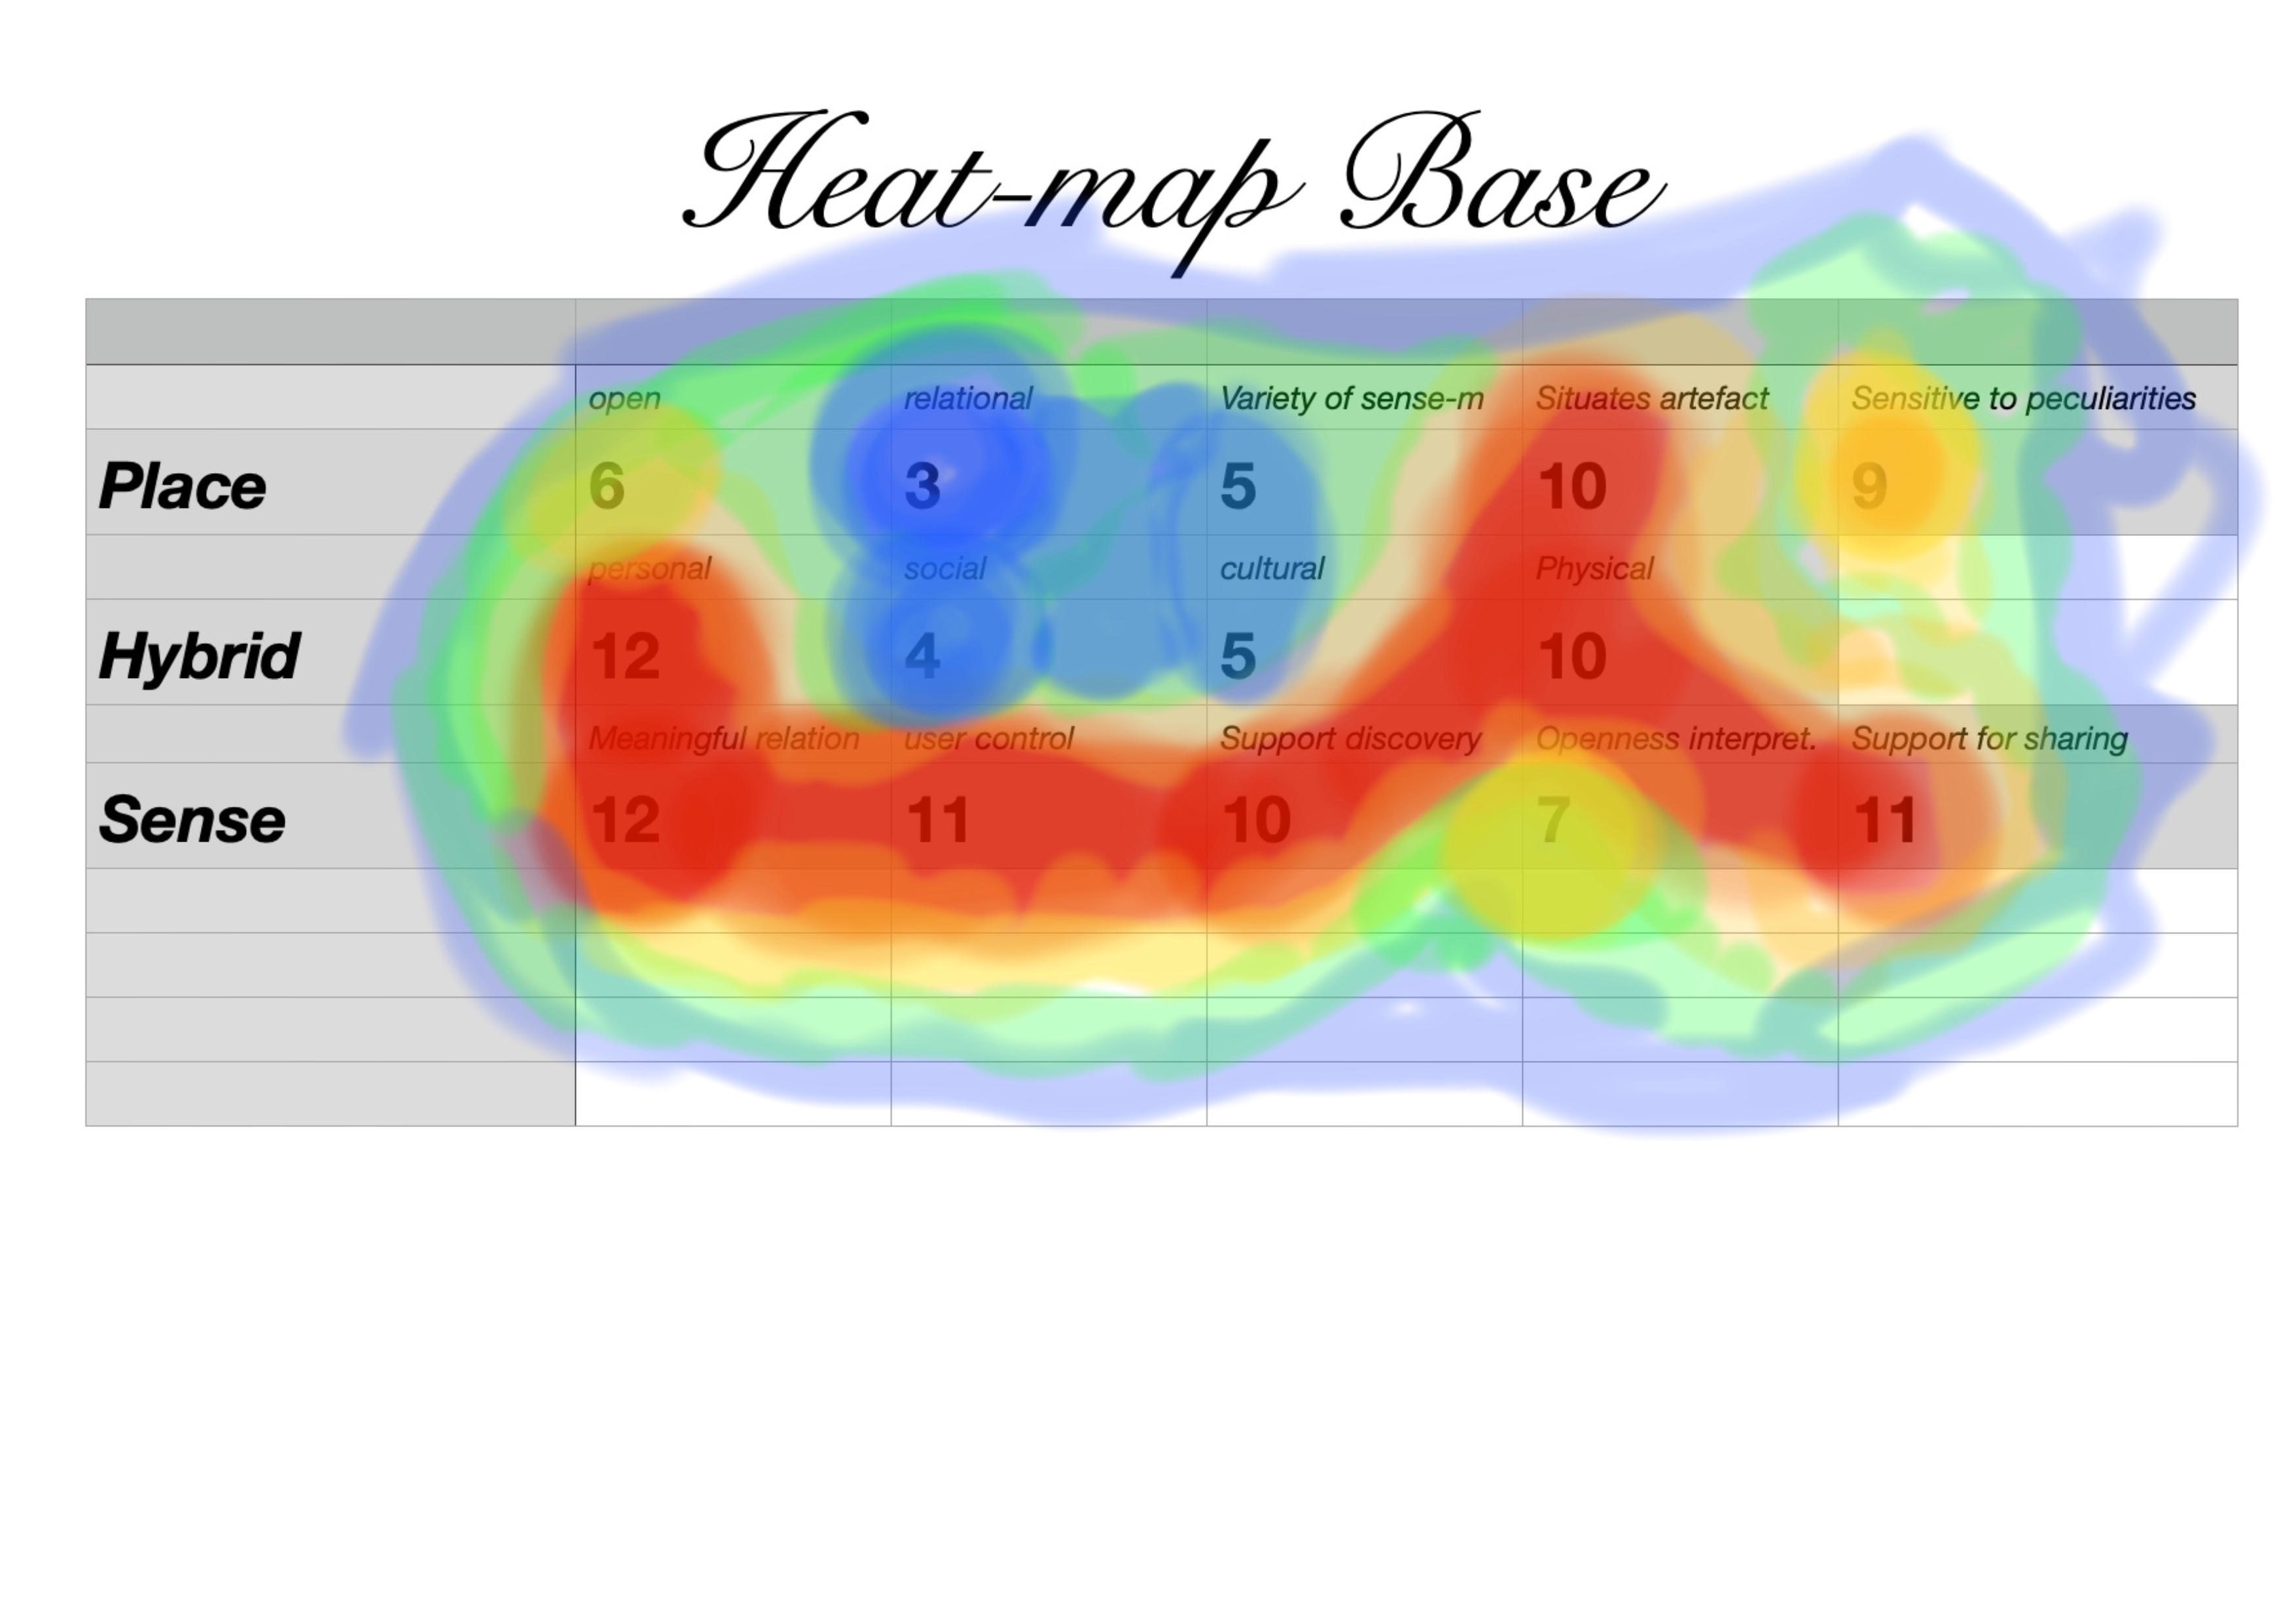
\includegraphics[width=11cm]{pictures/dataset/heatmap.jpg}
\centering 
\end{figure}


\section{First iteration: seeing the bigger picture}

I started the first analytical iteration by sorting the dataset into the three theories I base my understanding of meaningfulness on; \emph{Hybrid place, place as a dialogue} and \emph{Sense-making strategies}. I made one table for each theory, where the frameworks's principles/ and dimensions formed the columns and the 22 different installations the rows. I then went through each installation and plotted in whether or not the installation fulfilled the principle/ dimension. Categorising it this way opened up for looking at the dataset in correlation with each theory separately, making it possible to see overall trends in the dataset according to the theories. Another


respective theory from a birds-eye, holistic, perspective, but it will also work as a quick-reference guide for the second analysis iteration when I'm trying to merge the three theories and/ or finding new relationships between the data across the theories.

The categorisation of the data is highly subjective, but theoretically grounded, based on my personal experience with- and interpretation of the installations and knowledge of the museum institution the installation was part of. I have also chosen to merge all the Munch - \emph{Shadows} installations as one, because they are a part of the same exhibition and do not differ in their interactive qualities. Because of this, the dataset used for this analysis shrinked from 22 to 16. This choice of merging the \emph{Shadows} installations was made in the process of fitting the installations into the theory's principles/ dimensions, when I saw that they all checked the same boxes. 


\begin{figure}[H]
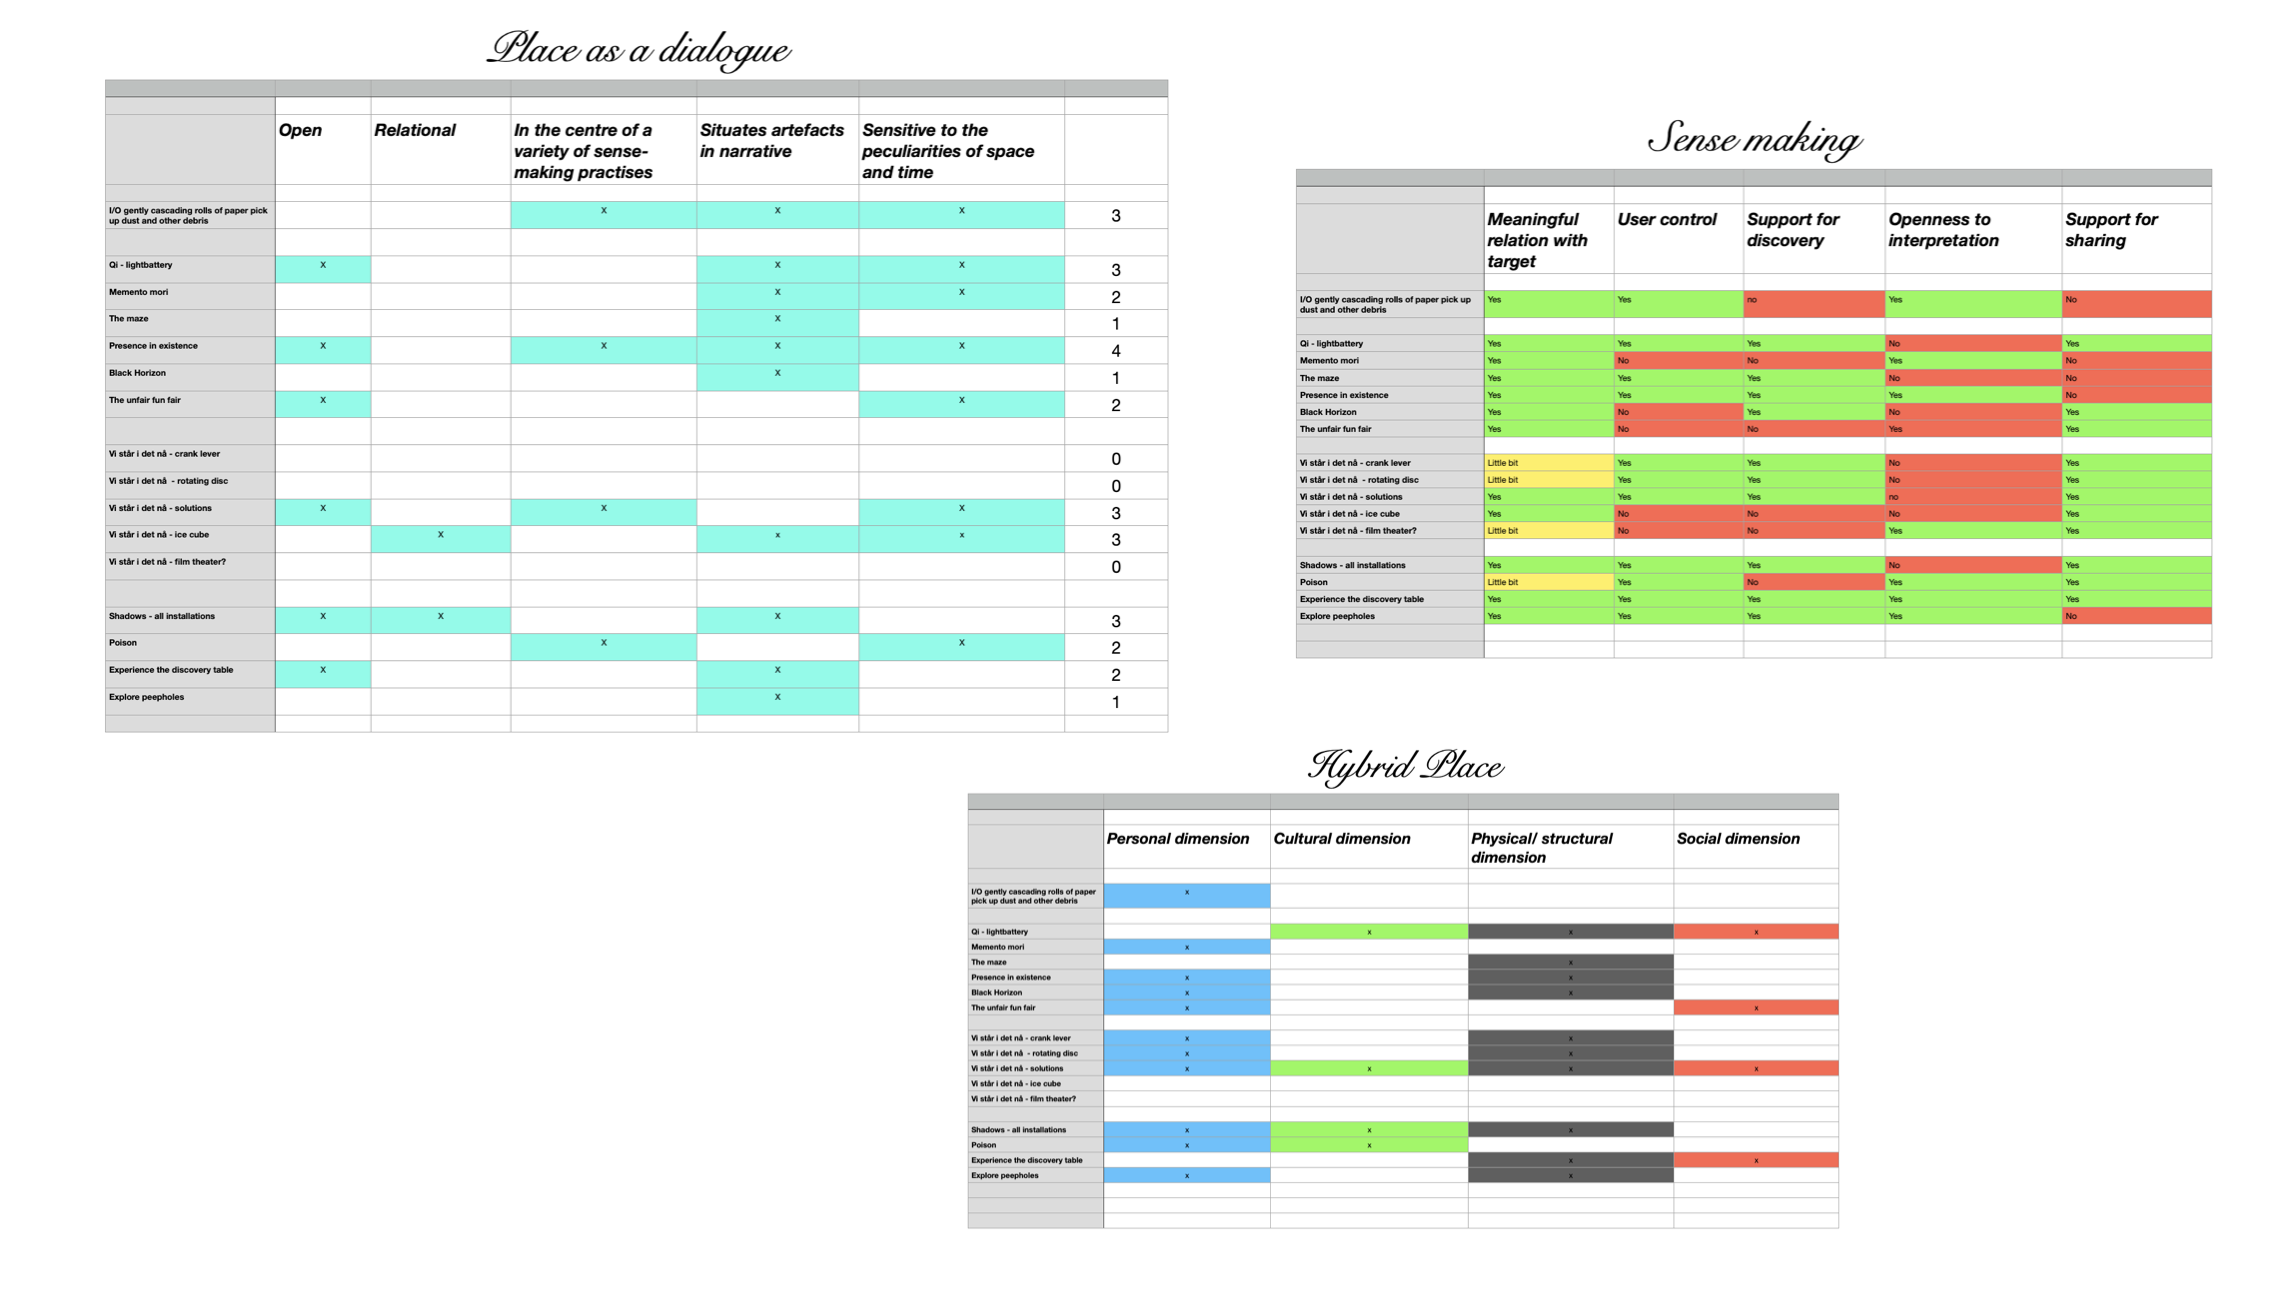
\includegraphics[width=13cm]{pictures/dataset/analysis_tables.png}
\centering 
\end{figure}

After mapping the installations in the tables, it opened up for crunching the first numbers. In this iteration I want to see the dataset from a holistic view. Abstracting from the details and seeing how the installations map up in the bigger picture. To do this I needed a diagram that could compare the different principles up against eachother. I chose to create radar charts to do this, and made a radar chart for each theory. 

\begin{figure}[H]
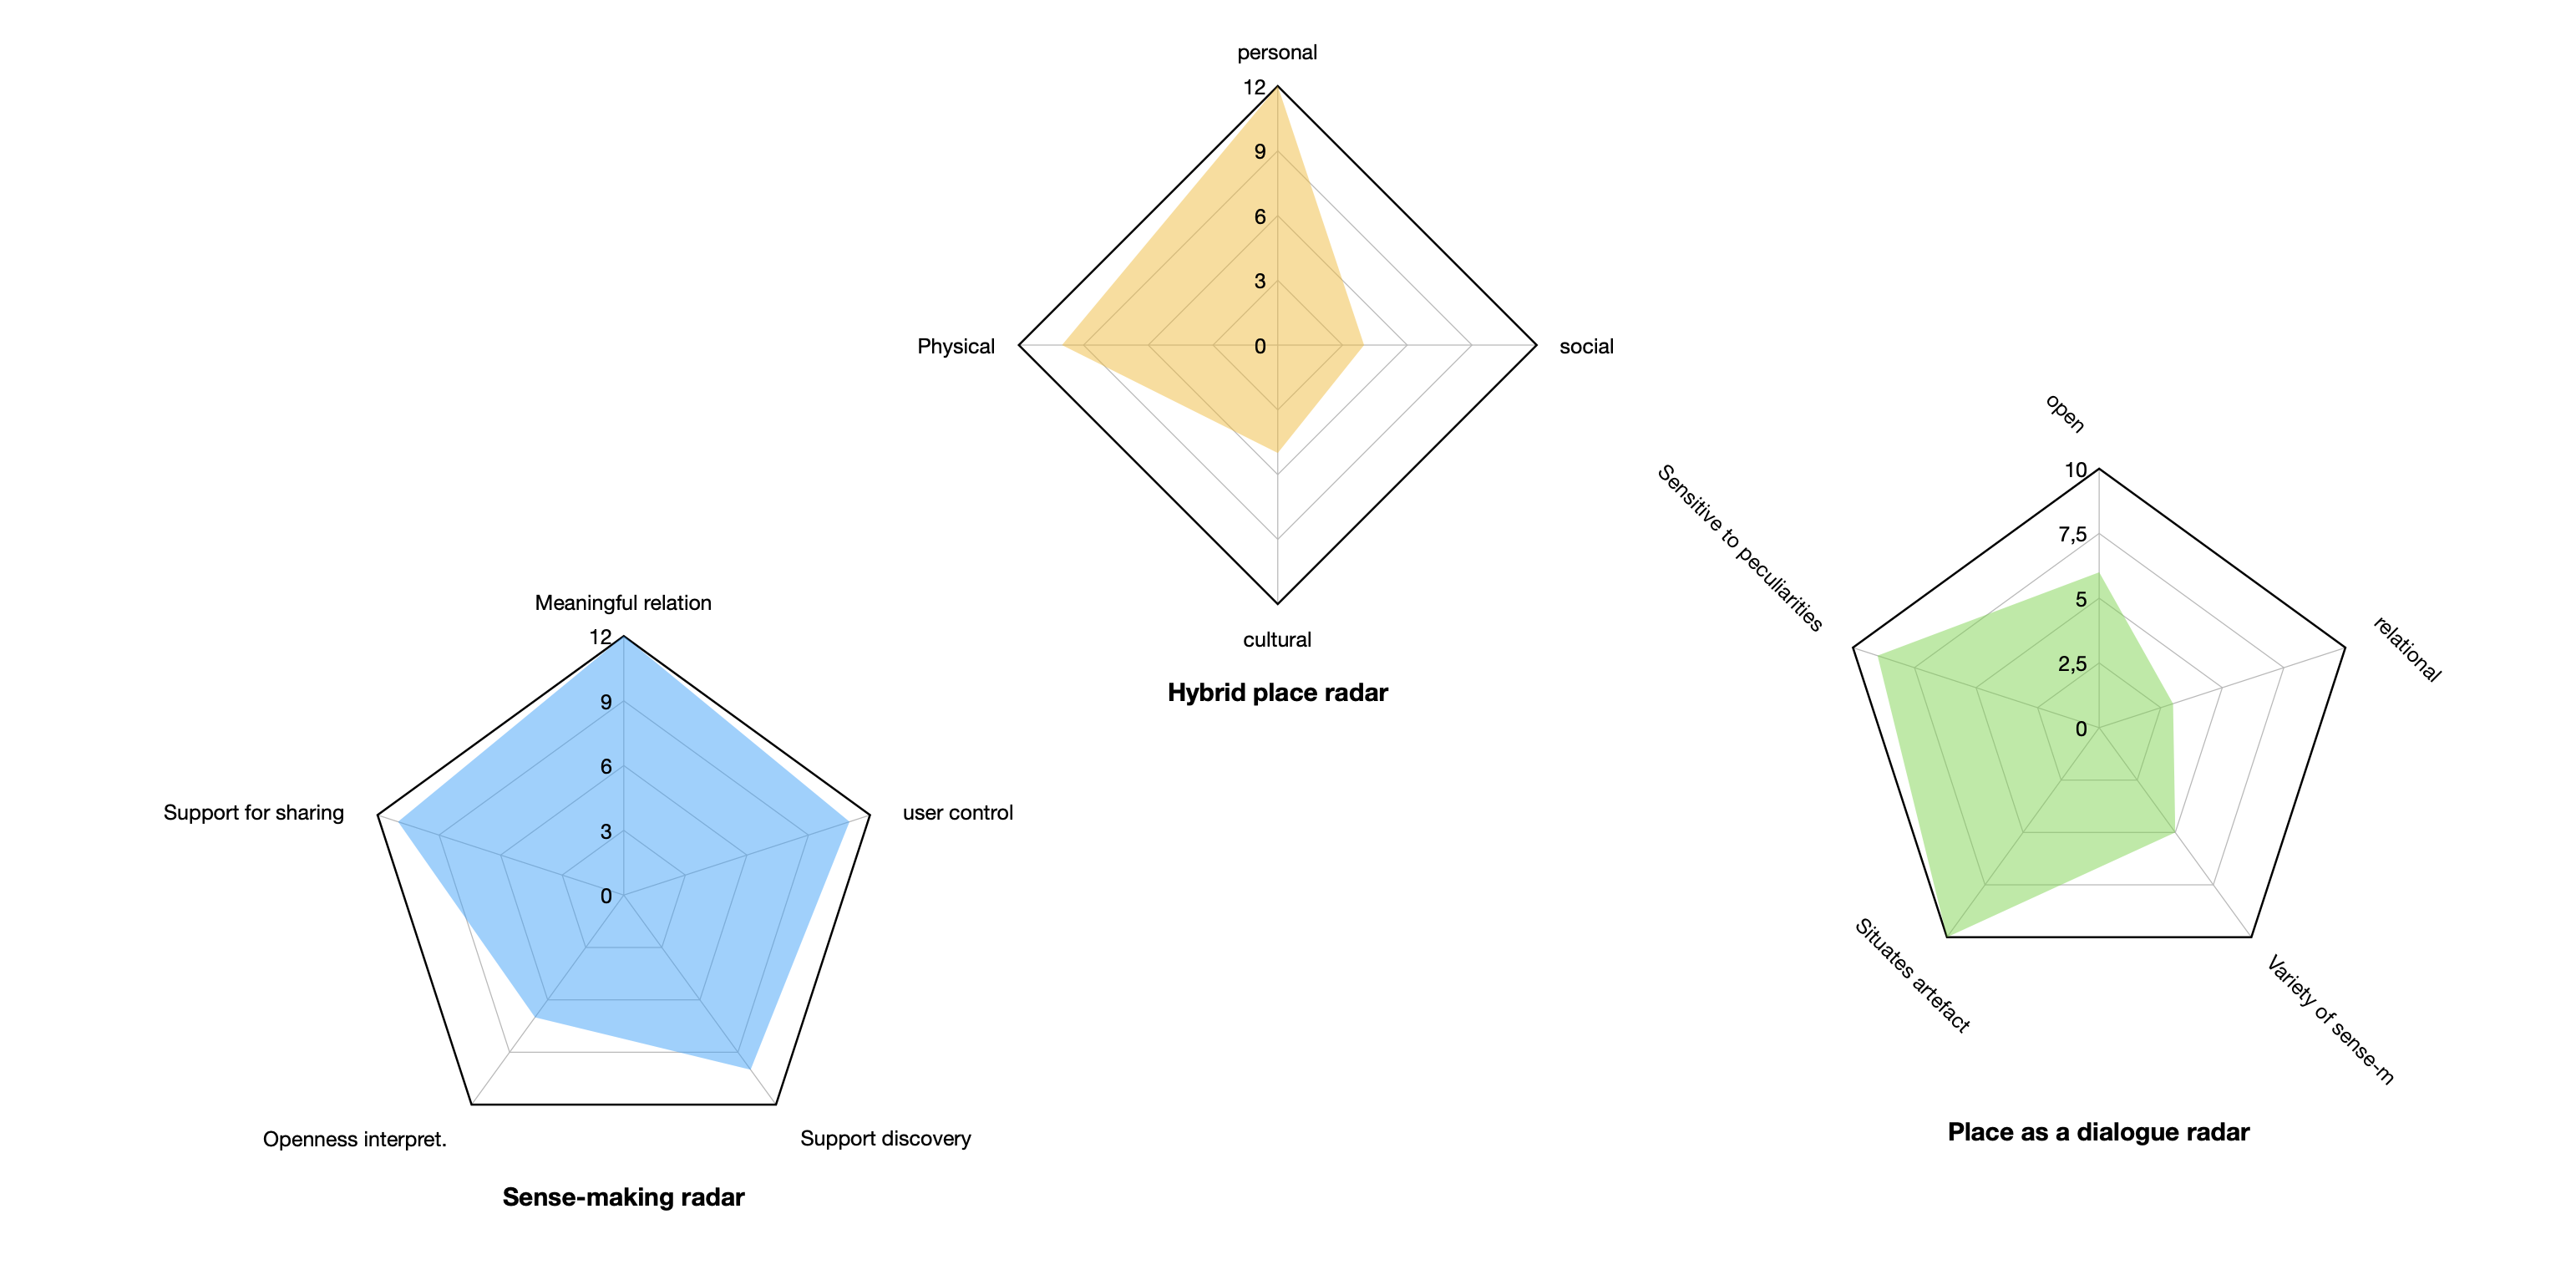
\includegraphics[width=13cm]{pictures/dataset/analysis_radars.png}
\centering 
\end{figure}

\emph{"Findings"}
\par

What I have learned by looking at the radar charts so far is how the different theories fulfill, or complement eachother. The way I have gone forward in looking at the radar charts is as following:
\par I'll start by looking at the hybrid place radar chart, noticing how the personal and physical dimension is fulfilled, while the social and cultural dimension is very little fulfilled. What does this mean? According to the Norwegian museum policy strategic thinking, it is wanted that museums transition from the personal dimension to the more social and cultural dimension. The fact that installations in my analysis shows presence in the physical dimension is positive, in terms of enabling the personal dimension, experience-wise, to involve more tangible or at least dynamic experiences in the museum space.
\par Then, if we shift focus for a second to look into the sense-making radar chart, we see that one of the corners that is fulfilled by almost all installations in this analysis - support for sharing is fulfilled. How come, that even though the social dimension is not fulfilled while almost all installations, in terms of sense-making have good support for sharing? 

\par Then again, we can look at what dialogic qualities the installations turns out to have little "relationalness", which is a dialogic principle/ quality that involves the Docents in the museum for example, or relational qualitites.




\chapter{\ding{167} Discussion}
In this chapter we look back at the thesis project and discuss it.

\section{So, how can one design for meaningful interactive experiences in a museum space that addresses sustainability?}



\subsection{Research question evolution and documentation}

\textbf{Research as a creative, generative process}
Documentation --> the researchers basis for contributions (\emph{the research}). In research through design, the documentation also play a creative and generative role - because it is involved as part as a design process just as much as the research process.
In a way, I see the research question as something "levende", fluid, that is not static. 
Forskning er en generativ prosess - science is a generative and creative process.
Perhaps also say something about autoethnography/ biography?
"The inner-organisation of the portfolio is annotated to make it communicable to other people (researchers, designers, users, whoever). Effective annotation will also enable comparative work" \autocite[p. 72]{bowers_annotated_2012}. 



\subsection{Research through design, methodology}

The methodological approach in this thesis reflects the same challenges that is discussed in the literature in terms of doing 

The methodological approach in this thesis reflects the same challenges that is discussed in the literature in terms of doing research through design. Not only is there little 

A researcher's methodology allows the reader to understand the approach and methods used to reach conclusions. This is important in any academic discipline, an

A research methodology gives research legitimacy and provides scientifically sound findings. It also provides a detailed plan that helps to keep researchers on track, making the process smooth, effective and manageable. A researcher's methodology allows the reader to understand the approach and methods used to reach conclusions.

To showcase and give reason for the process and progress of any aca

In academic papers



The methodology for this study reflects the challenges resulting from the intersection between installation design, museum facilitating attitude change and sustainability as a contemporary, and complex (!), discourse. 

Liker ikke "fase-tenkningen" dems. Its difficult to lock and close the activities in a box!!

Research through design is a "radical" way of doing science. I think it is groundbreaking and paving a more authentic and selfless way of doing science. One of the things which makes RtD a different methodology than other is the focus on the designer/ scientist@s knowledge, and how subjective but theoretically grounded opinions and forces fulfil and complement the science project. 

Writing is a creative process, and scientist/ researchers are good writers. A lot of knowledge is produced during the writing process, and in traditional science this writing isnt appreciated enough. Writing is a creative process (method) where a lot of knowledge is processed and produced. In my opinion, RtD is recognising and acknowledging, legitimising, this knowledge producing process. Research, of all diciplines, should aim to rightfully showcase the knowledge-process that happens through writing and reading..  (literature review..)

Zimmerman and Forlizzi are one of "the big names" in terms of research through design in interaction design, hci, and I know they exist. However, I find their approach to be very analytical, and actually, a bit difficult to apply in a real-time project. Which is why I'd rather use a more open-ended way of describing my thesis process. 

I find Zimmerman and Forlizzi's model (define, discover, synthesize, construct, refine, reflect) difficult to be a good fit in terms of RtD's practical nature. Thinking and structuring the process in phases mean 



\section{The "practical" researcher}
Early in the book Doing Ethnographies, we are introduced to the concepts of ‘the detached researcher’ and of ‘the pure subject’ which together adresses the power relations between the researcher and the research-subject. “Research is an embodied activity that draws in our whole physical person, along with all its inescapable identities. (…) what we bring to the research affects what we get .“(Crang and Cook, 2007, p. 9). I have most definitely brought with me biases, opinions and attitudes toward the theme of sustainability, [...] which definitely framed the way I looked and inquired into the topic,

Limitations, scientist role on the debate and as a researcher, specifically related to the climate debate:
“What’s the motivation? True, research has become a political or resource issue, as much as an academic one. And, as a slight digression, it always amuses me to see the word ‘academic’ used as a pejorative - by people who themselves earn their livings within the academy. Research has become a status issue, as much as a conceptual or even practical one. And that - I must confess - worries me.” \autocite[p. 5]{frayling_1994}. This is quite interesting, and in some way, it could also be something we see the consequences of in regards to the ongoing climate debates where scientists are doubted and not trusted. That the science they predict feels more like a hoax. Perhaps this mistrust is somewhat manifested through this stereotypical description that Frayling describes.

\subsection{What designers make of what they see}
% If relevant, add citation to bibliography
Jane F. Suri writes in her article Poetic Observation: What Designers Make of What They See(2011), that “Designers need to interpret what they see (and otherwise sense) in ways that will lead to design outcomes.” Which is especially true for me and the outcome of my thesis, and also why I need to be aware and critical of my role and values as a researcher, because  I am the one shaping and deciding how and what the aspects of the installation that adresses sustainability should be. Suri further emphasises how interpreting what we see is both a personal and a social process, and that “In our own individual ways, all of us pay attention to what’s meaningful and interesting to us. While we might guess that certain activities will be fruitful, not everyone sees the same things or finds them equally useful.”(Suri, 2011, p. 18).

Jane Fulton-Suri, reflecting on her training in social science followed by her experience working at a design consultancy, identified a gap between design with its focus on the future and social science research with its focus on the past and present \autocite[p. 167]{zimmerman_research_2014}.

\subsubsection{Has research become a status issue?}

Fraylings questioning of research becoming a status issue have been a perspective in the back of my mind 

\emph{"Where the tradition is concerned, one interesting question is why people want to call it research with a big 'r' at all. Whats the motivation? True, research has become a political or resource issue, as much as an academic one. And, as a slight digression, it always amuses me to see the word 'academic' used as a pejorative - by people who themselves earn their livings within the academy. Research has become a status issue as much as a conceptual or even practical one. And that - I must confess - worries me. There may well be opportunities for research within the expressive tradition, but they need dispassionate research, rather than heated discussion about status, class and reverse snobbery"} \autocite[p. 5]{frayling_1994}.

\par

\begin{comment}
\subsection{form, fit, context: learning about the context }

I believe, as a first step, it is important to try to be as fully immersed in the existing context of ‘what Klimahuset is’, as possible. Before thinking about what form the installation should have, I need a thorough understanding of the context the installation is to be placed in, to be able to start shaping the form. The existing context will also set some constraints for what kind of fit the installation will have in the context, a fit that will be continually evaluated throughout the design process. 


In the documents I have gotten access to from Klimahuset, there is a great focus on the buildings architecture. Design and architecture goes hand in hand, and the architectural outline of the exhibition space, sets creative constraints and limits for what the installation can be. It is also the “opportunity space” (mulighetsrom) I have available in the design of the installation. It is therefore important for me to know the “material”, thoughts and reasoning behind it.
\end{comment}


\chapter{\ding{167} Conclusion}
This thesis has considered the development and shift in museology practise while making clear a stronger connection between the Interaction Design / HCI field and museology. This has been explored through sustainability as a representative discourse being disseminated in museums, as a catalysator and manifestation of how museums aim to better disseminate (show and tell) contemporary discourses in society. 

The aim has been to theorize a new way to look at meaningfulness as a quality that you can design for, as a way to answer how one can design meaningful interactive experiences in a museum space that addresses sustainability. 



\backmatter{}

\printbibliography[nottype=online]
\printbibliography[type=online,title={Web sources}]

% \appendix
% \chapter{Appendix}
% \section{Three approaches to place-centred design}

% Hybrid place dimensions reference
% Place as dialogue reference

\section{Methodology & Process}
% zimmerman and Forlizzi (2004), knowledge opportunity map in the design process

\subsection{Klimahuset stories workshop dataset}

\subsubsection{Results from the Narrative Workshop}
\begin{figure}[H]
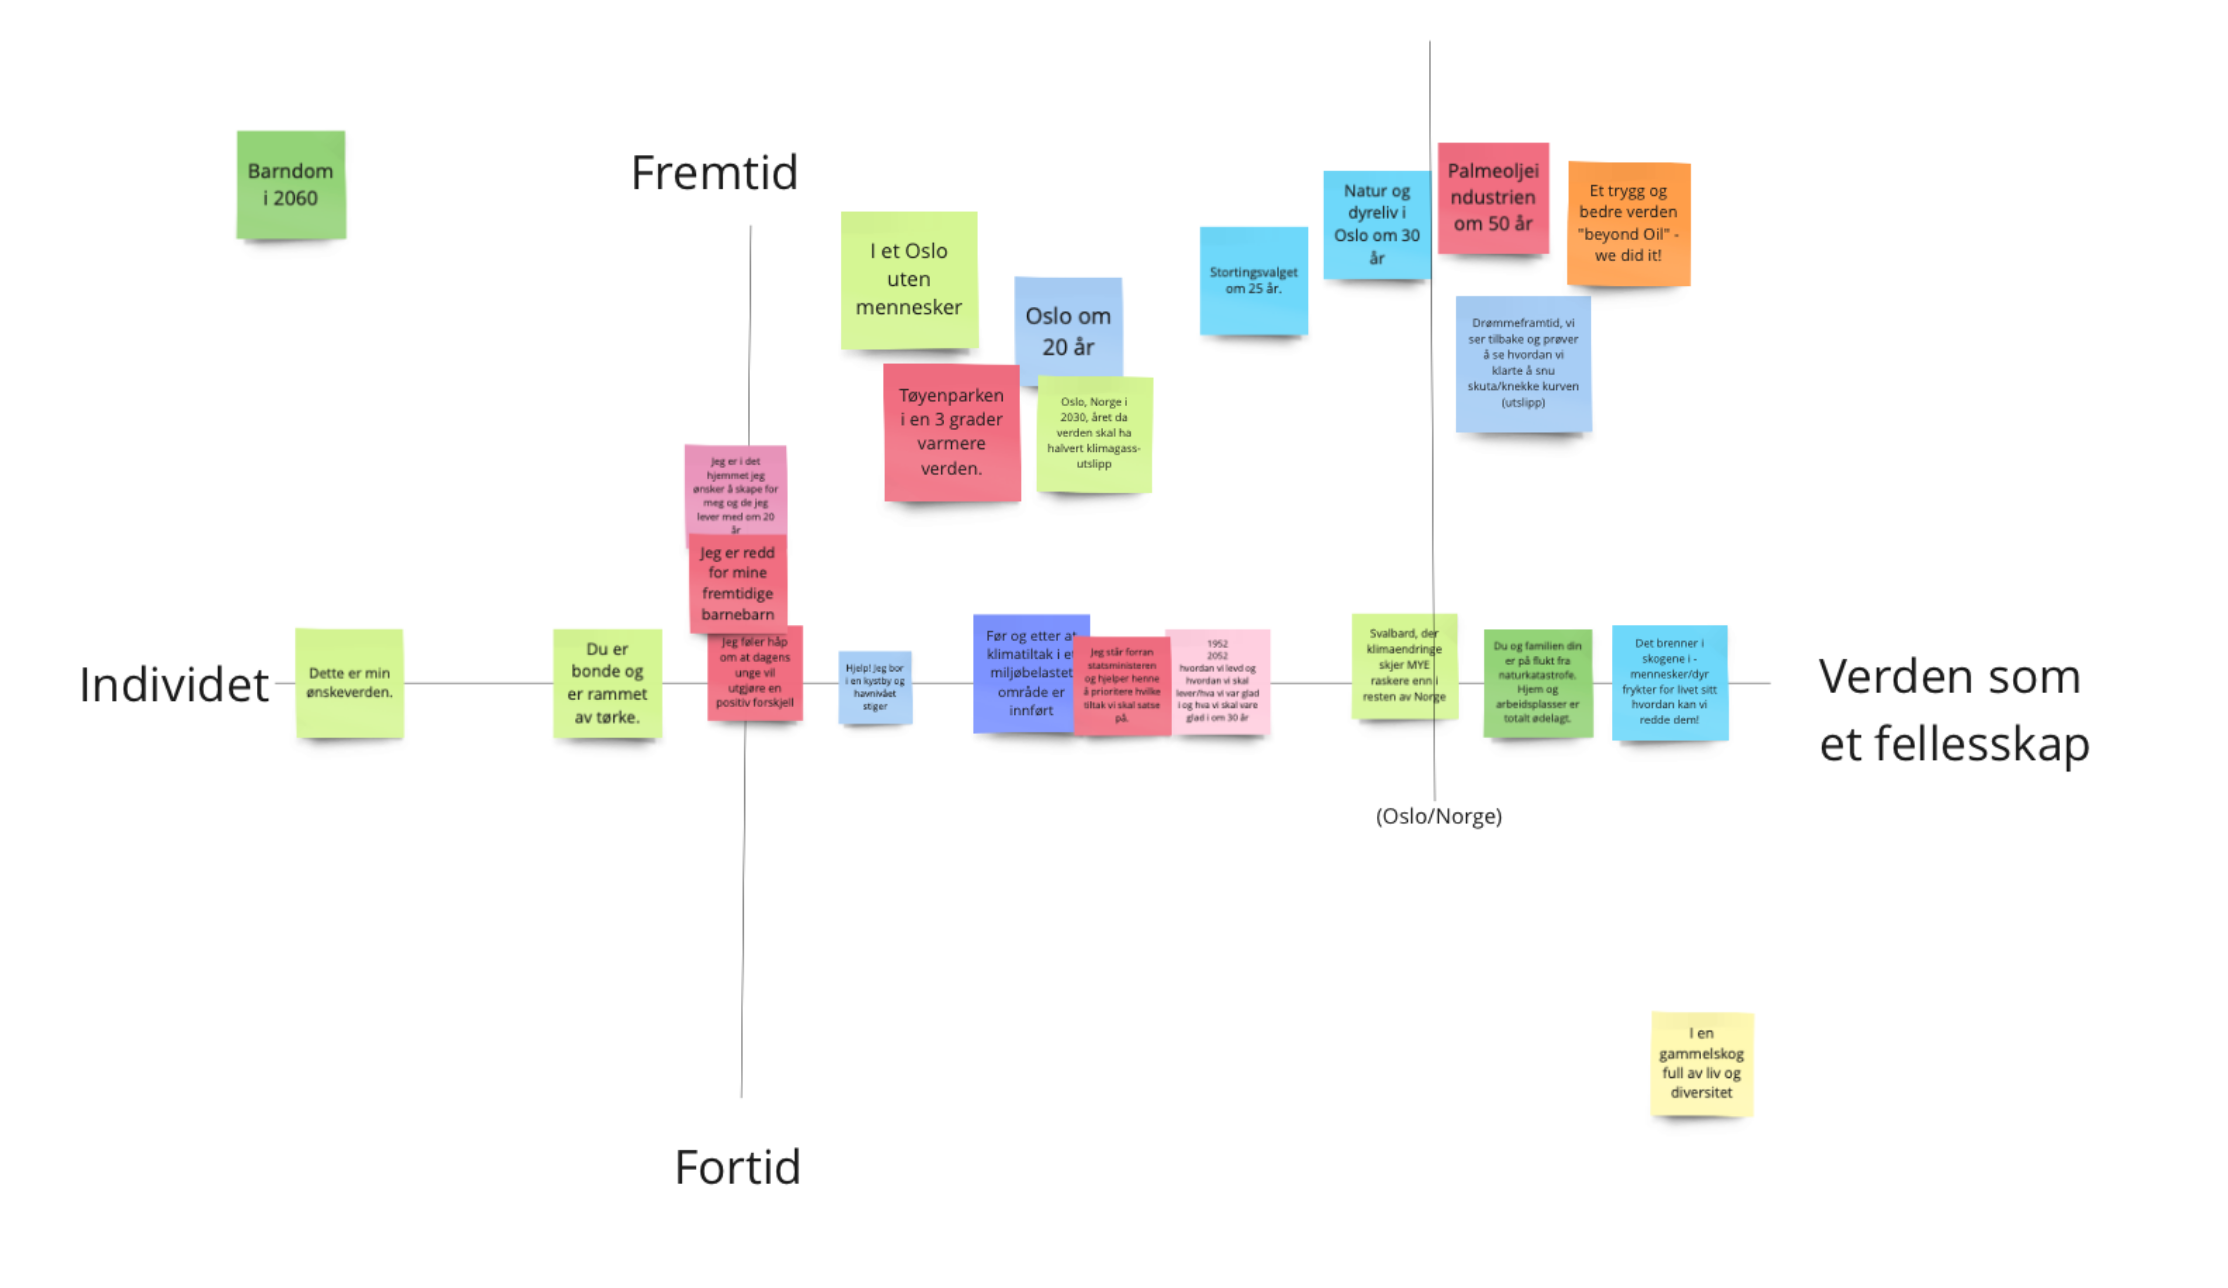
\includegraphics[width=12.5cm]{pictures/process/workshop_results.png}
\caption{Results from the Narrative Workshop described in section 8.2: Investigating narratives and storytelling with Klimahuset.}
\centering 
\end{figure}


\section{Analysis}
This section contains 

\begin{figure}[H]
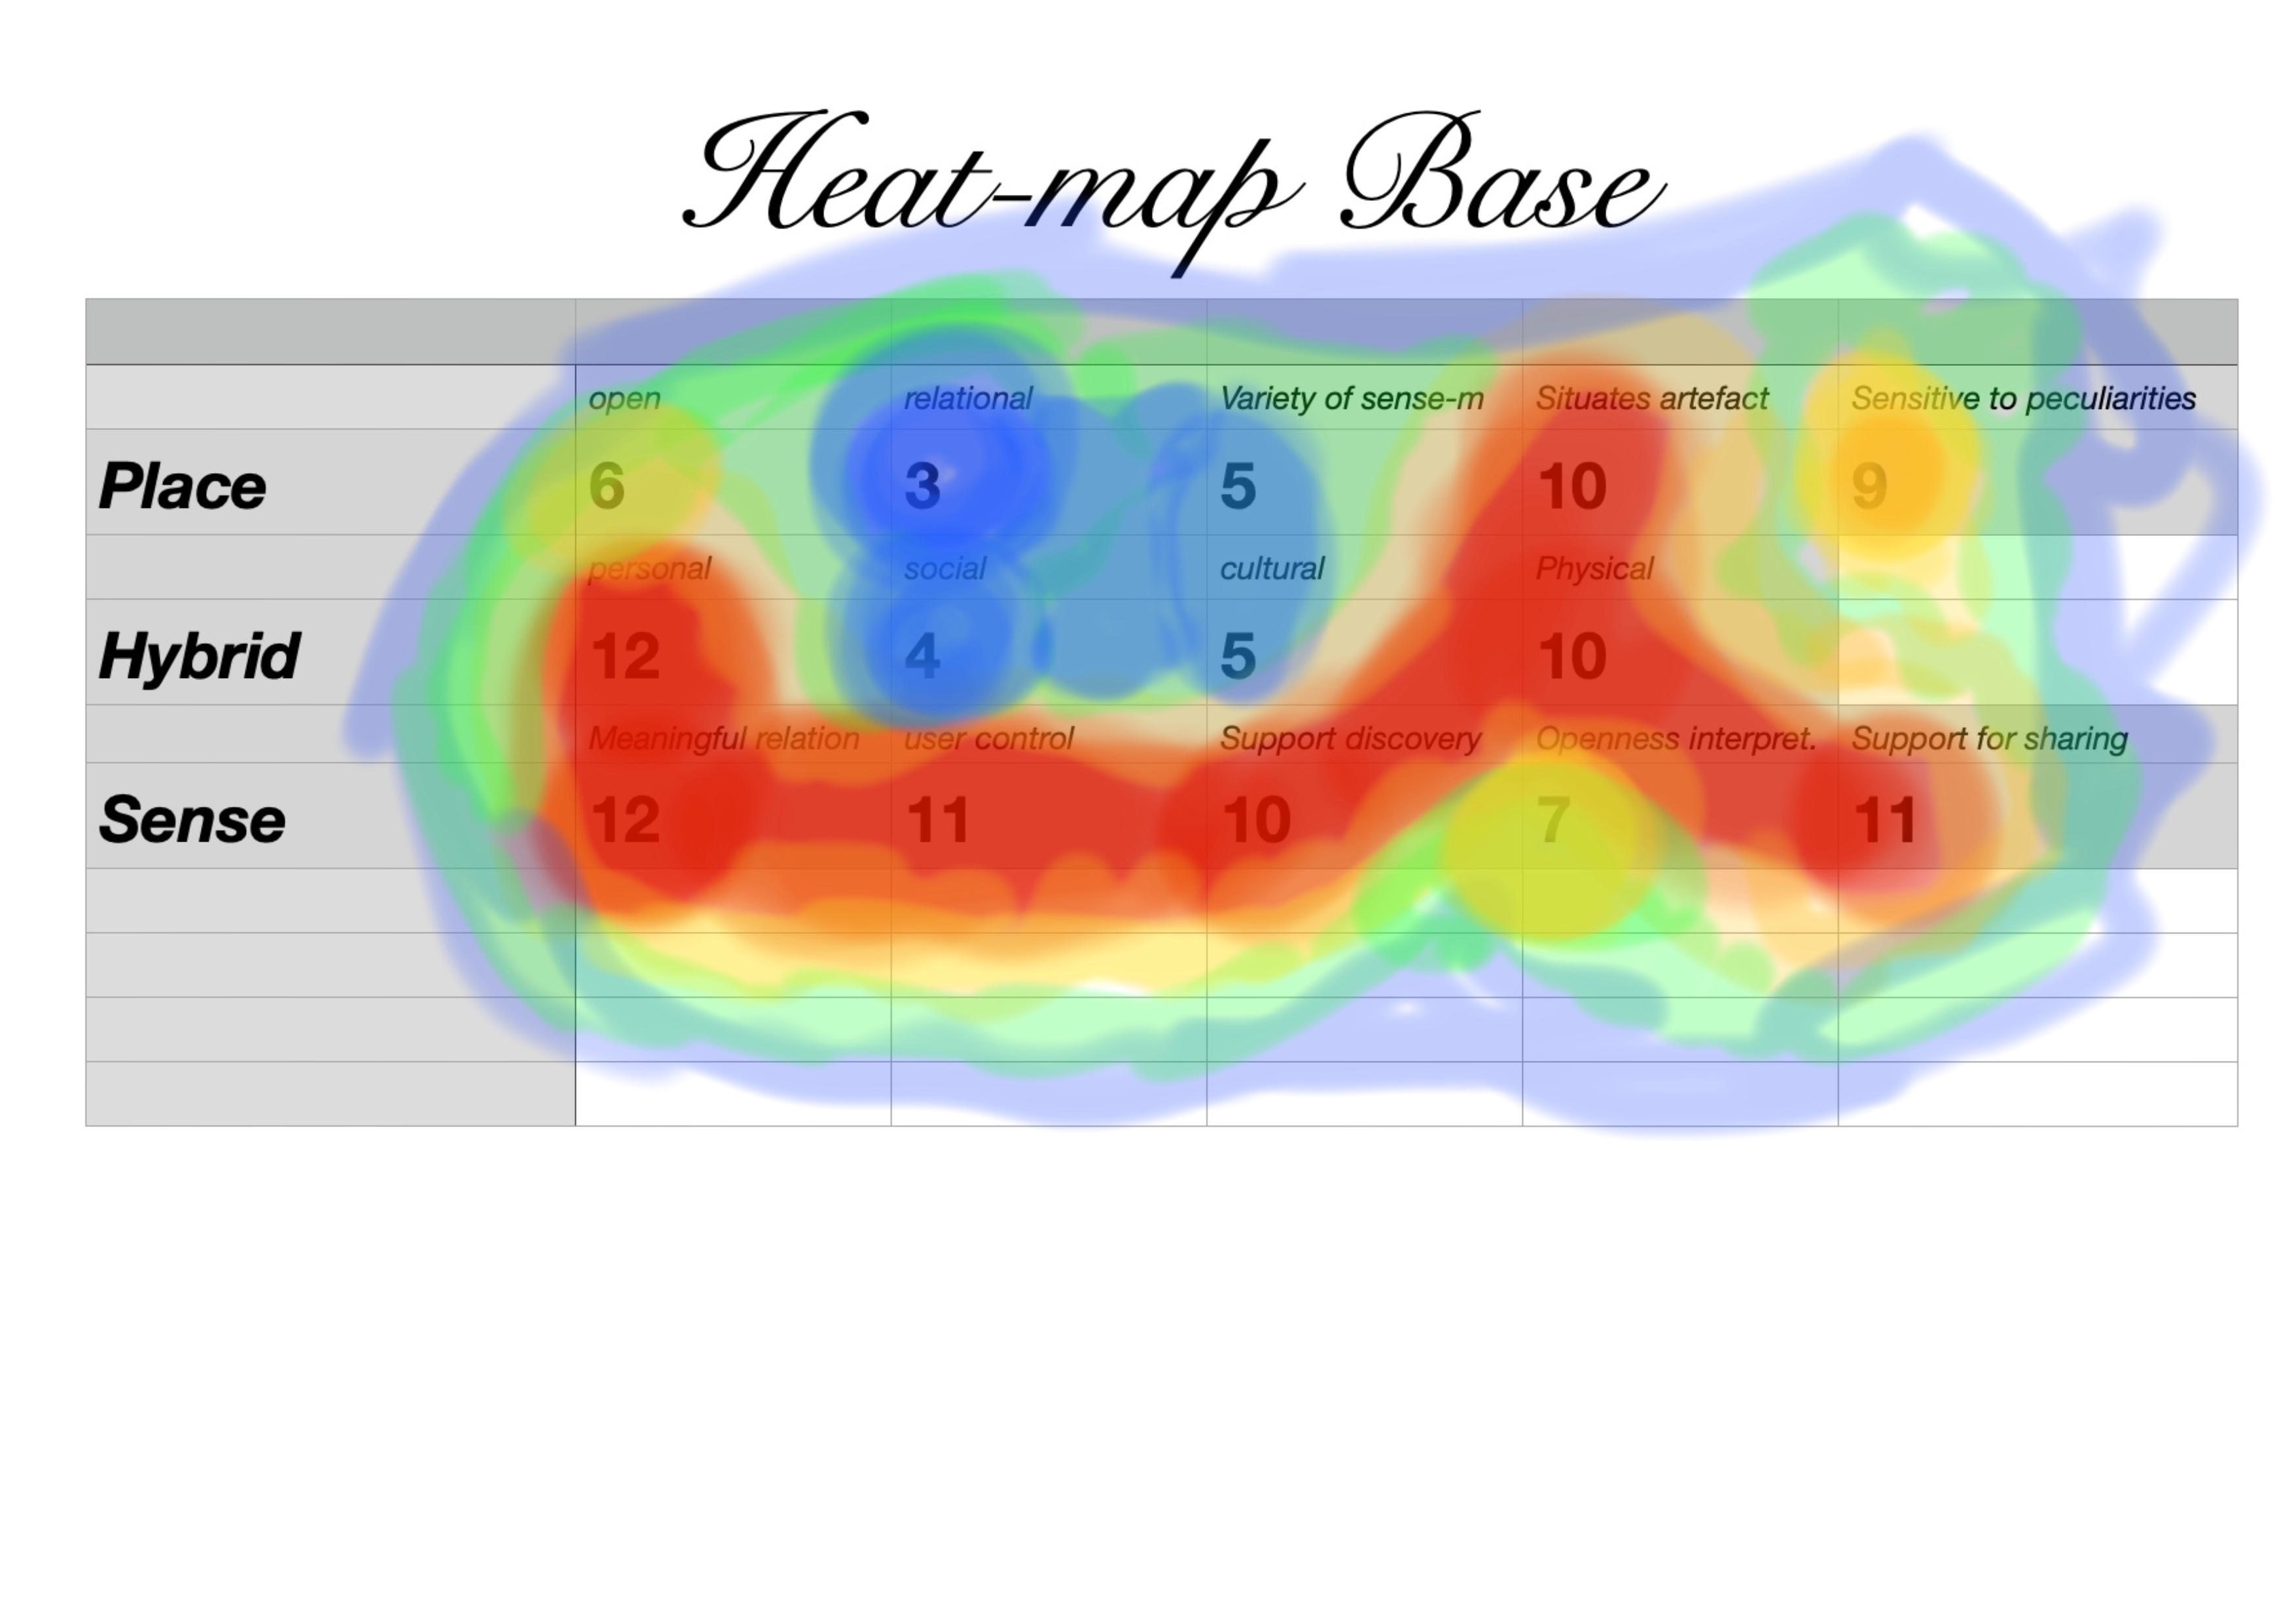
\includegraphics[width=12.5cm]{pictures/dataset/heatmap.jpg}
\caption{Heatmap version 1, Munch shadows is weighted as one}
\end{figure}

\section{Datagathering: observation guide}
\begin{figure}[H]
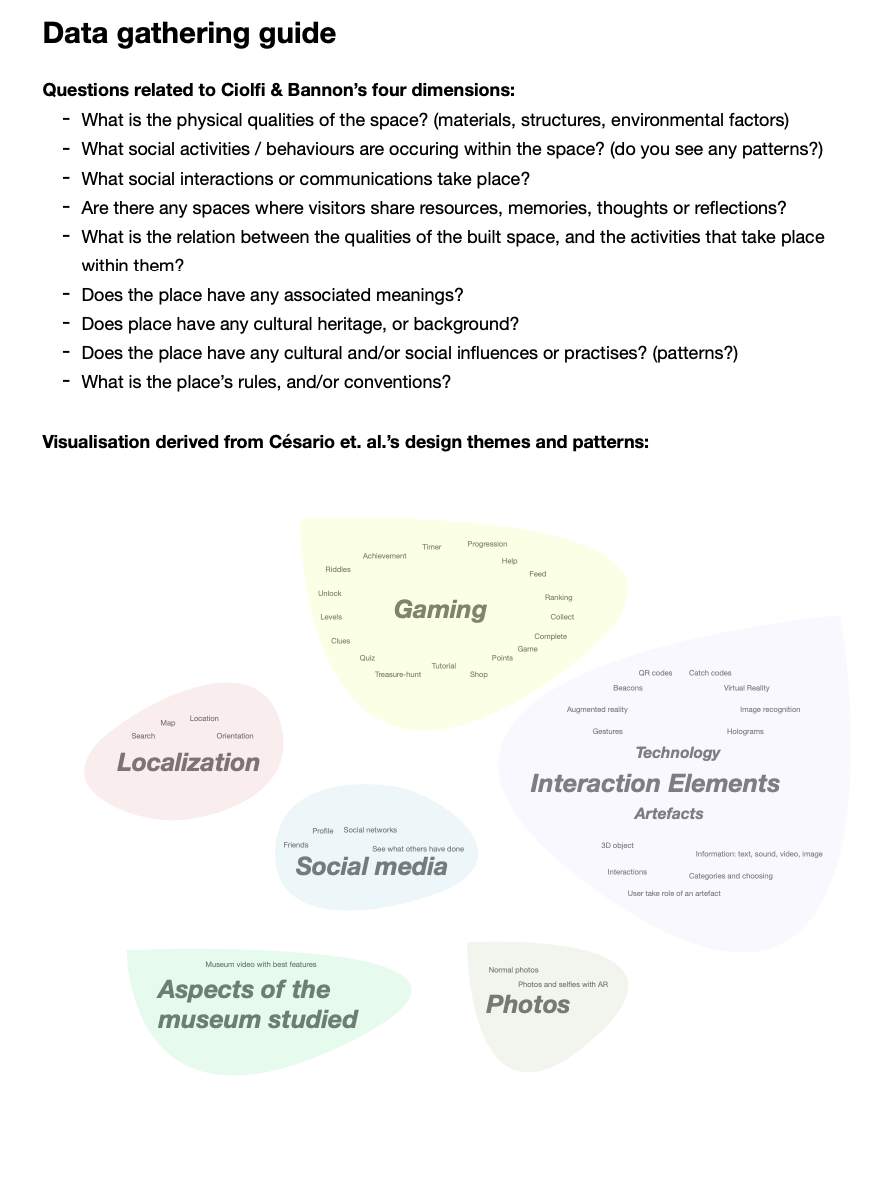
\includegraphics[width=13cm]{pictures/appendix/datagathering.png}
\centering 
\end{figure}

\section{Datagathering: interview guide}
\section{Dataset: Interactive Installations}

\begin{figure}[H]
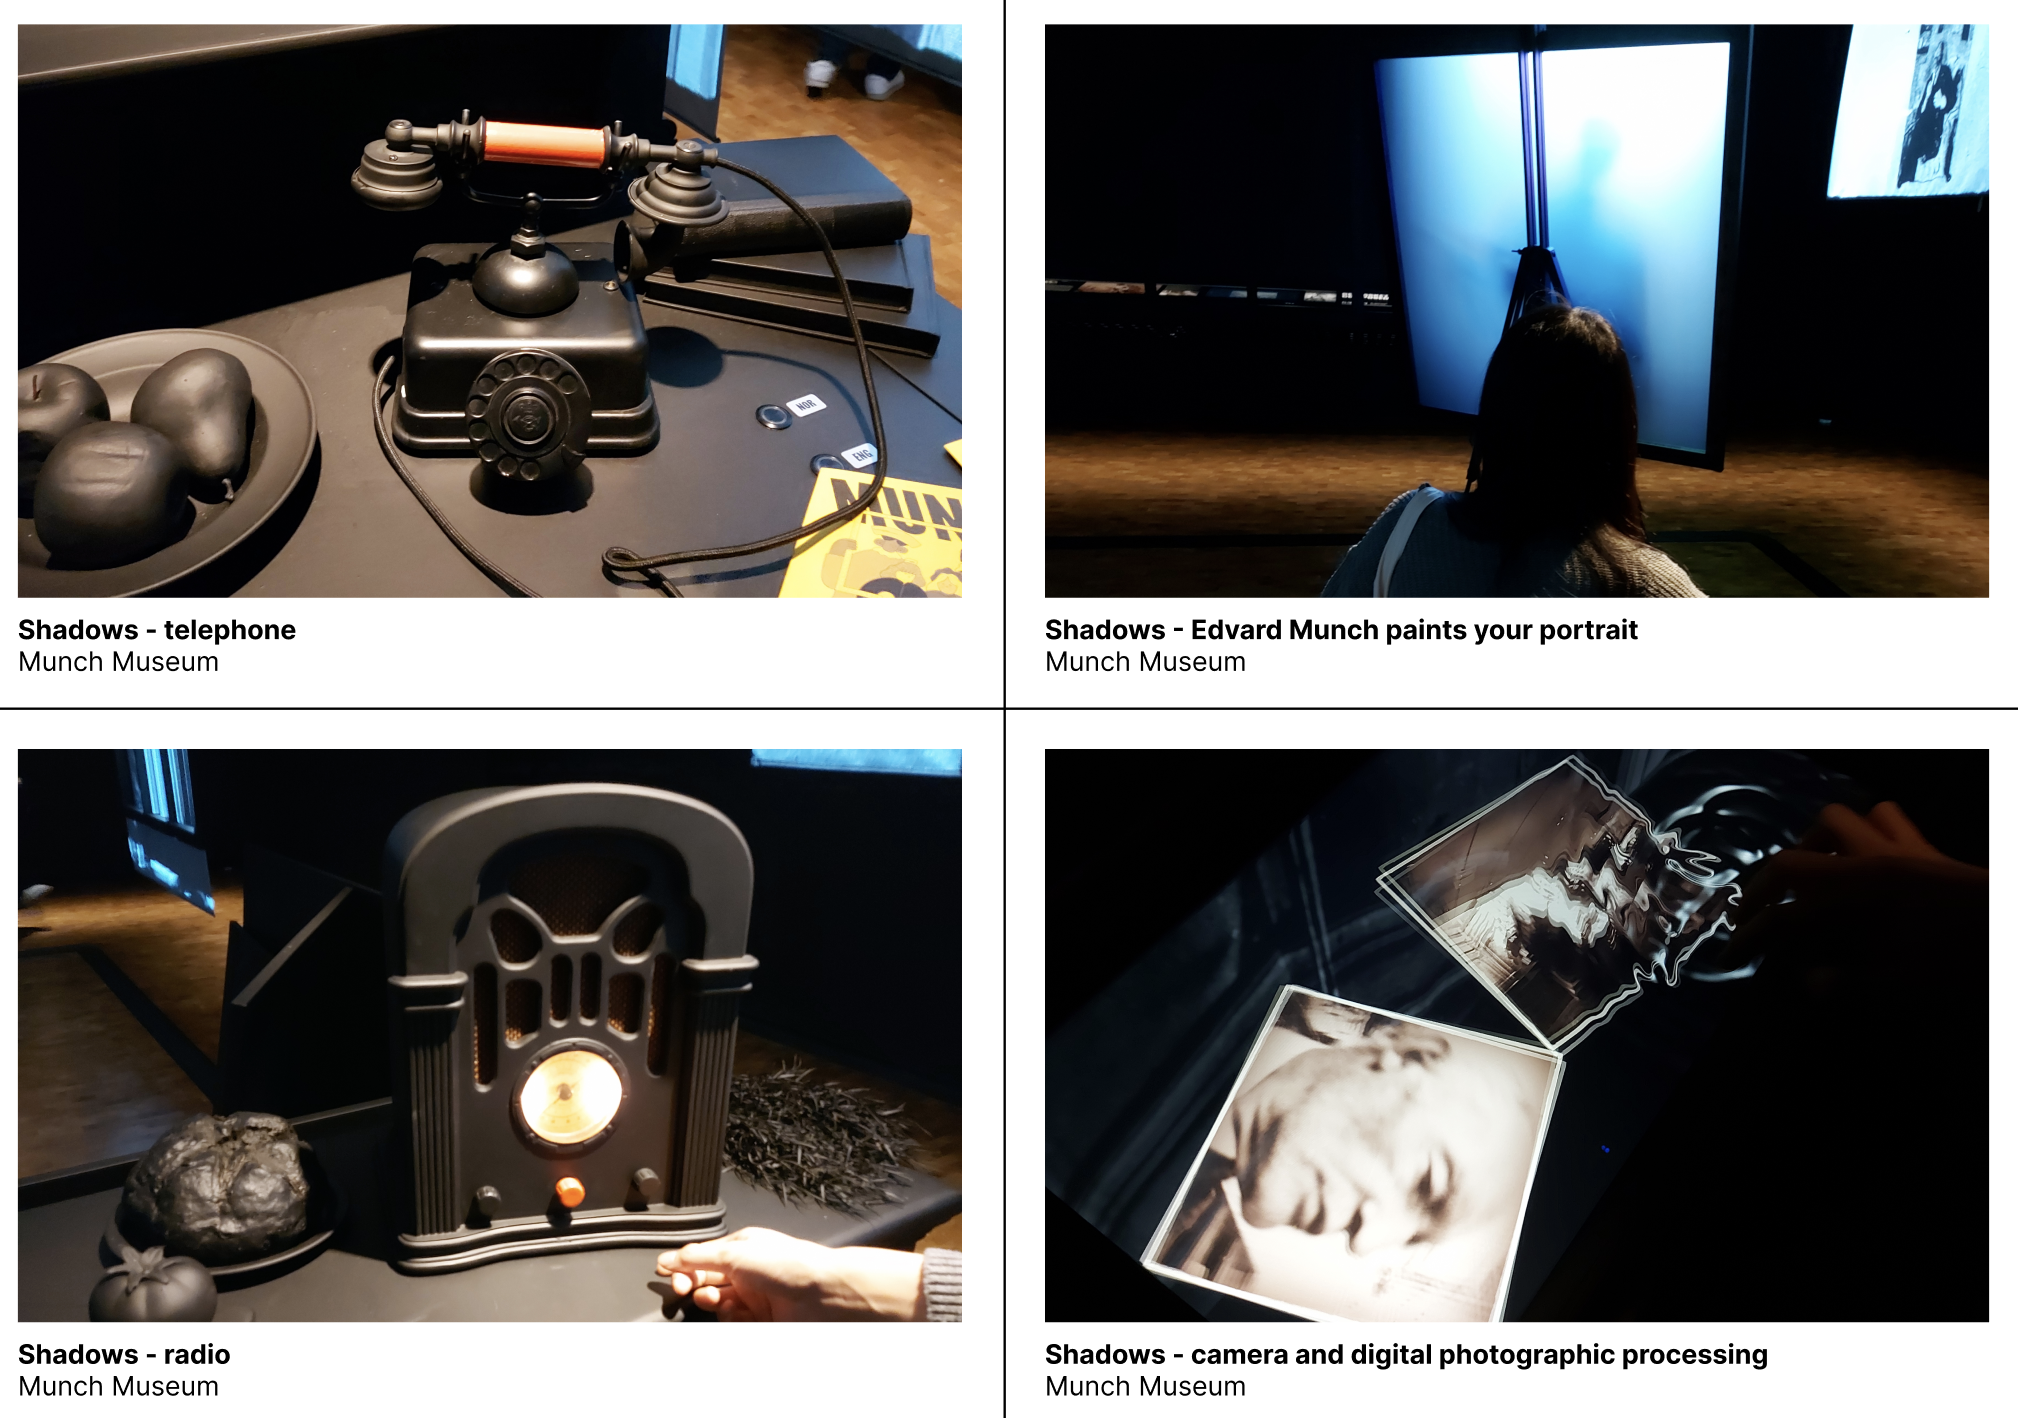
\includegraphics[width=13cm]{pictures/dataset/munch_1.png}
\centering 
\end{figure}

\begin{figure}[H]
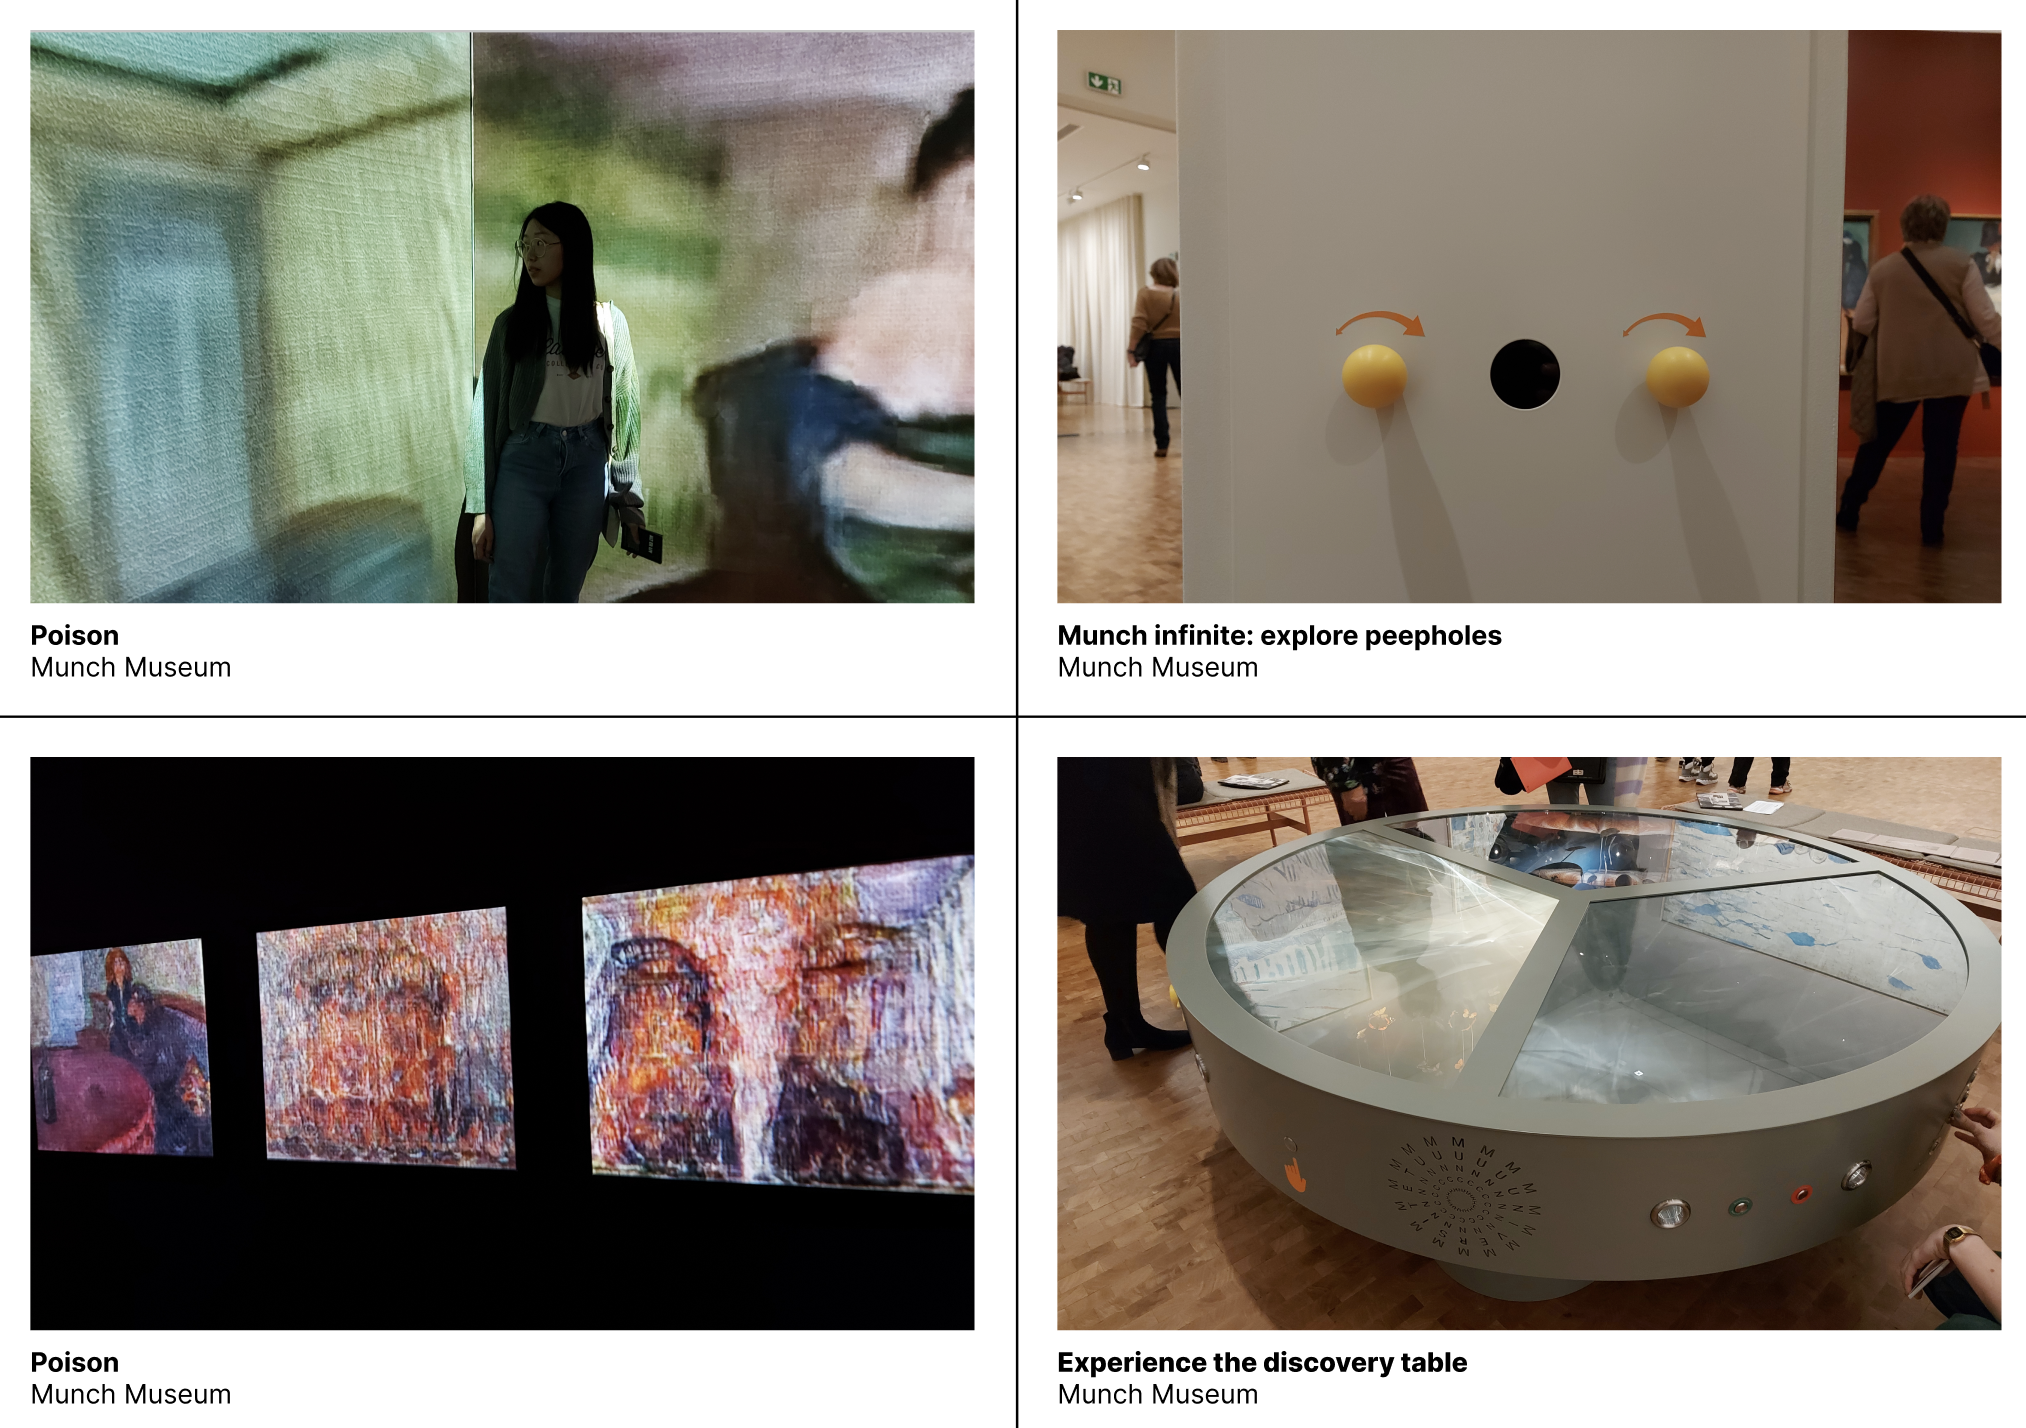
\includegraphics[width=13cm]{pictures/dataset/munch_2.png}
\centering 
\end{figure}

\begin{figure}[H]
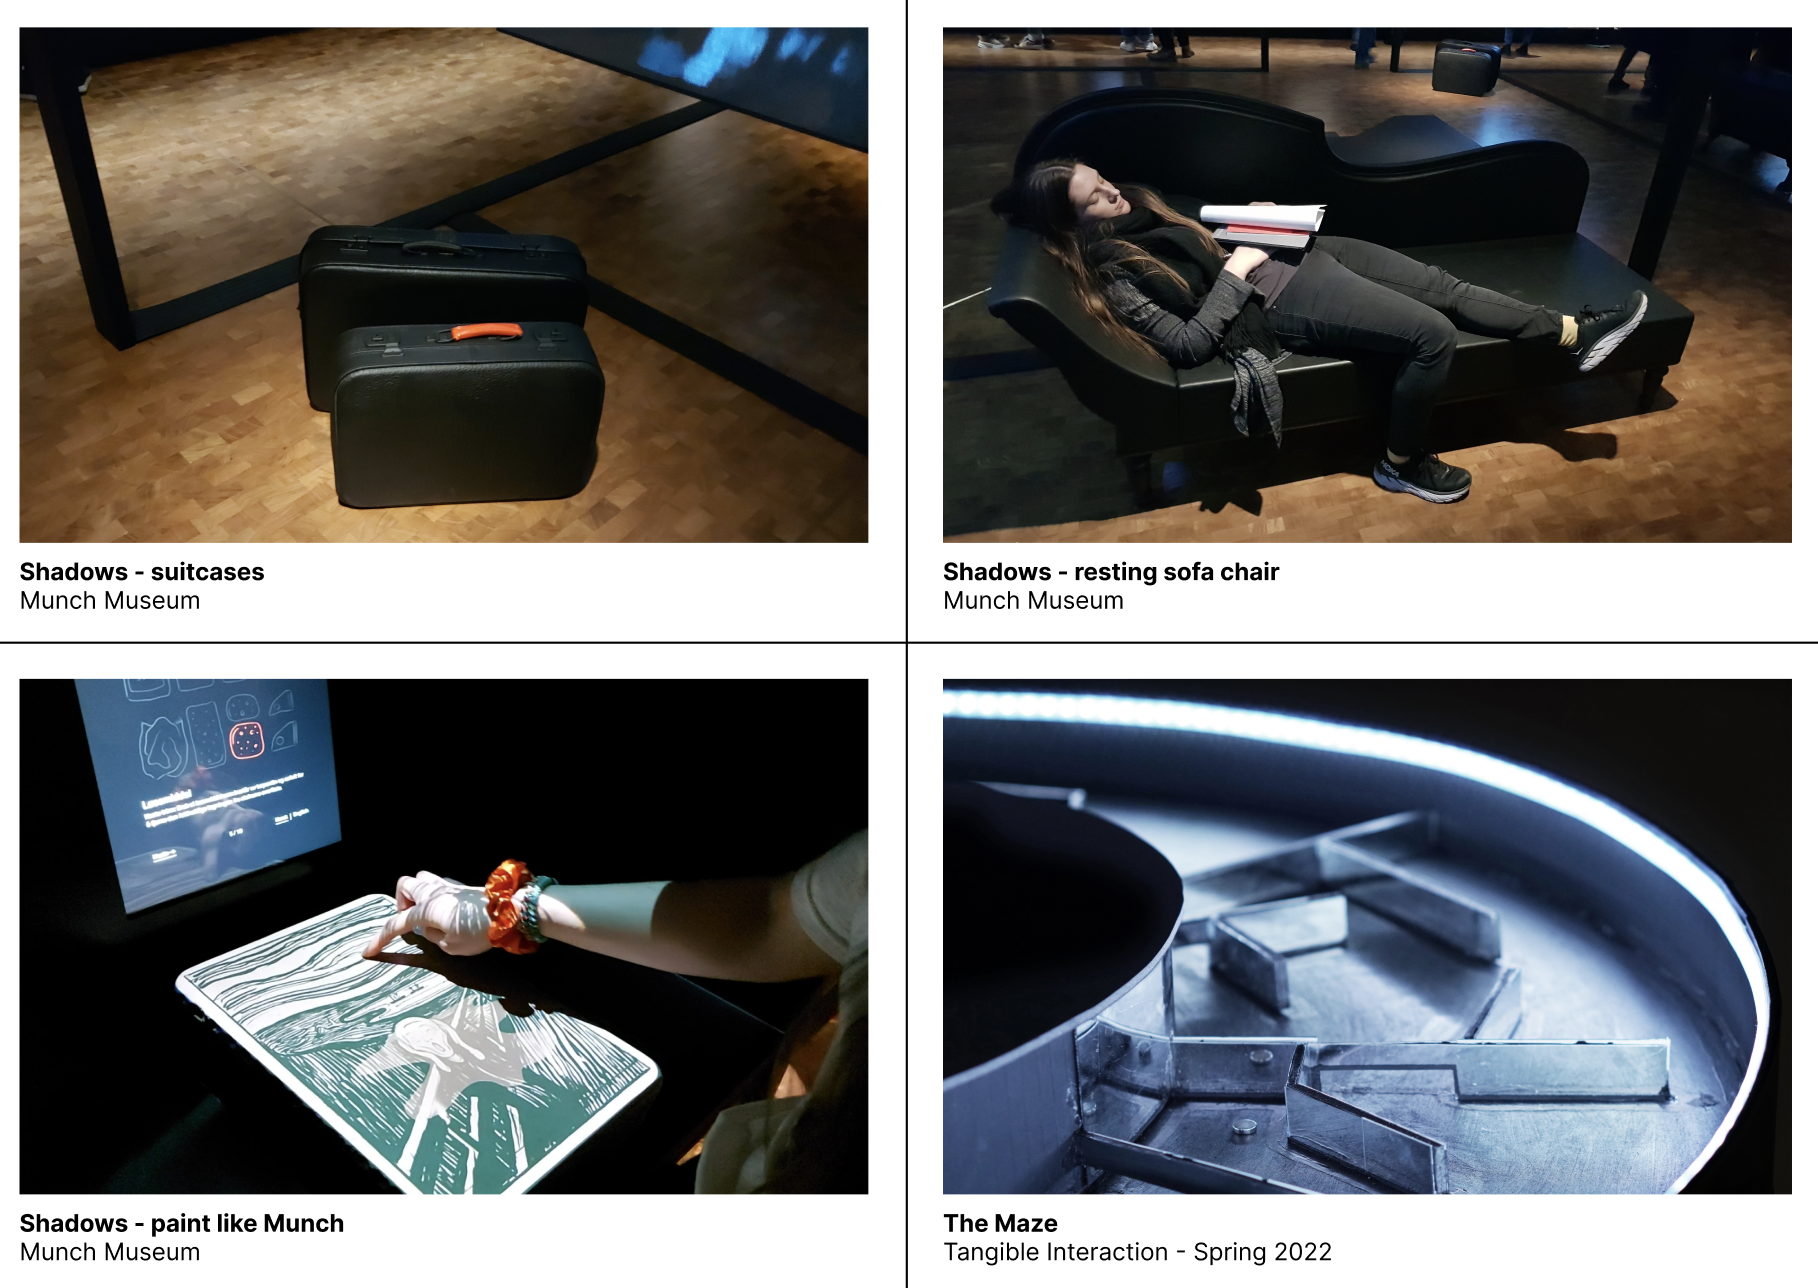
\includegraphics[width=13cm]{pictures/dataset/munch_3.png}
\centering 
\end{figure}

\begin{figure}[H]
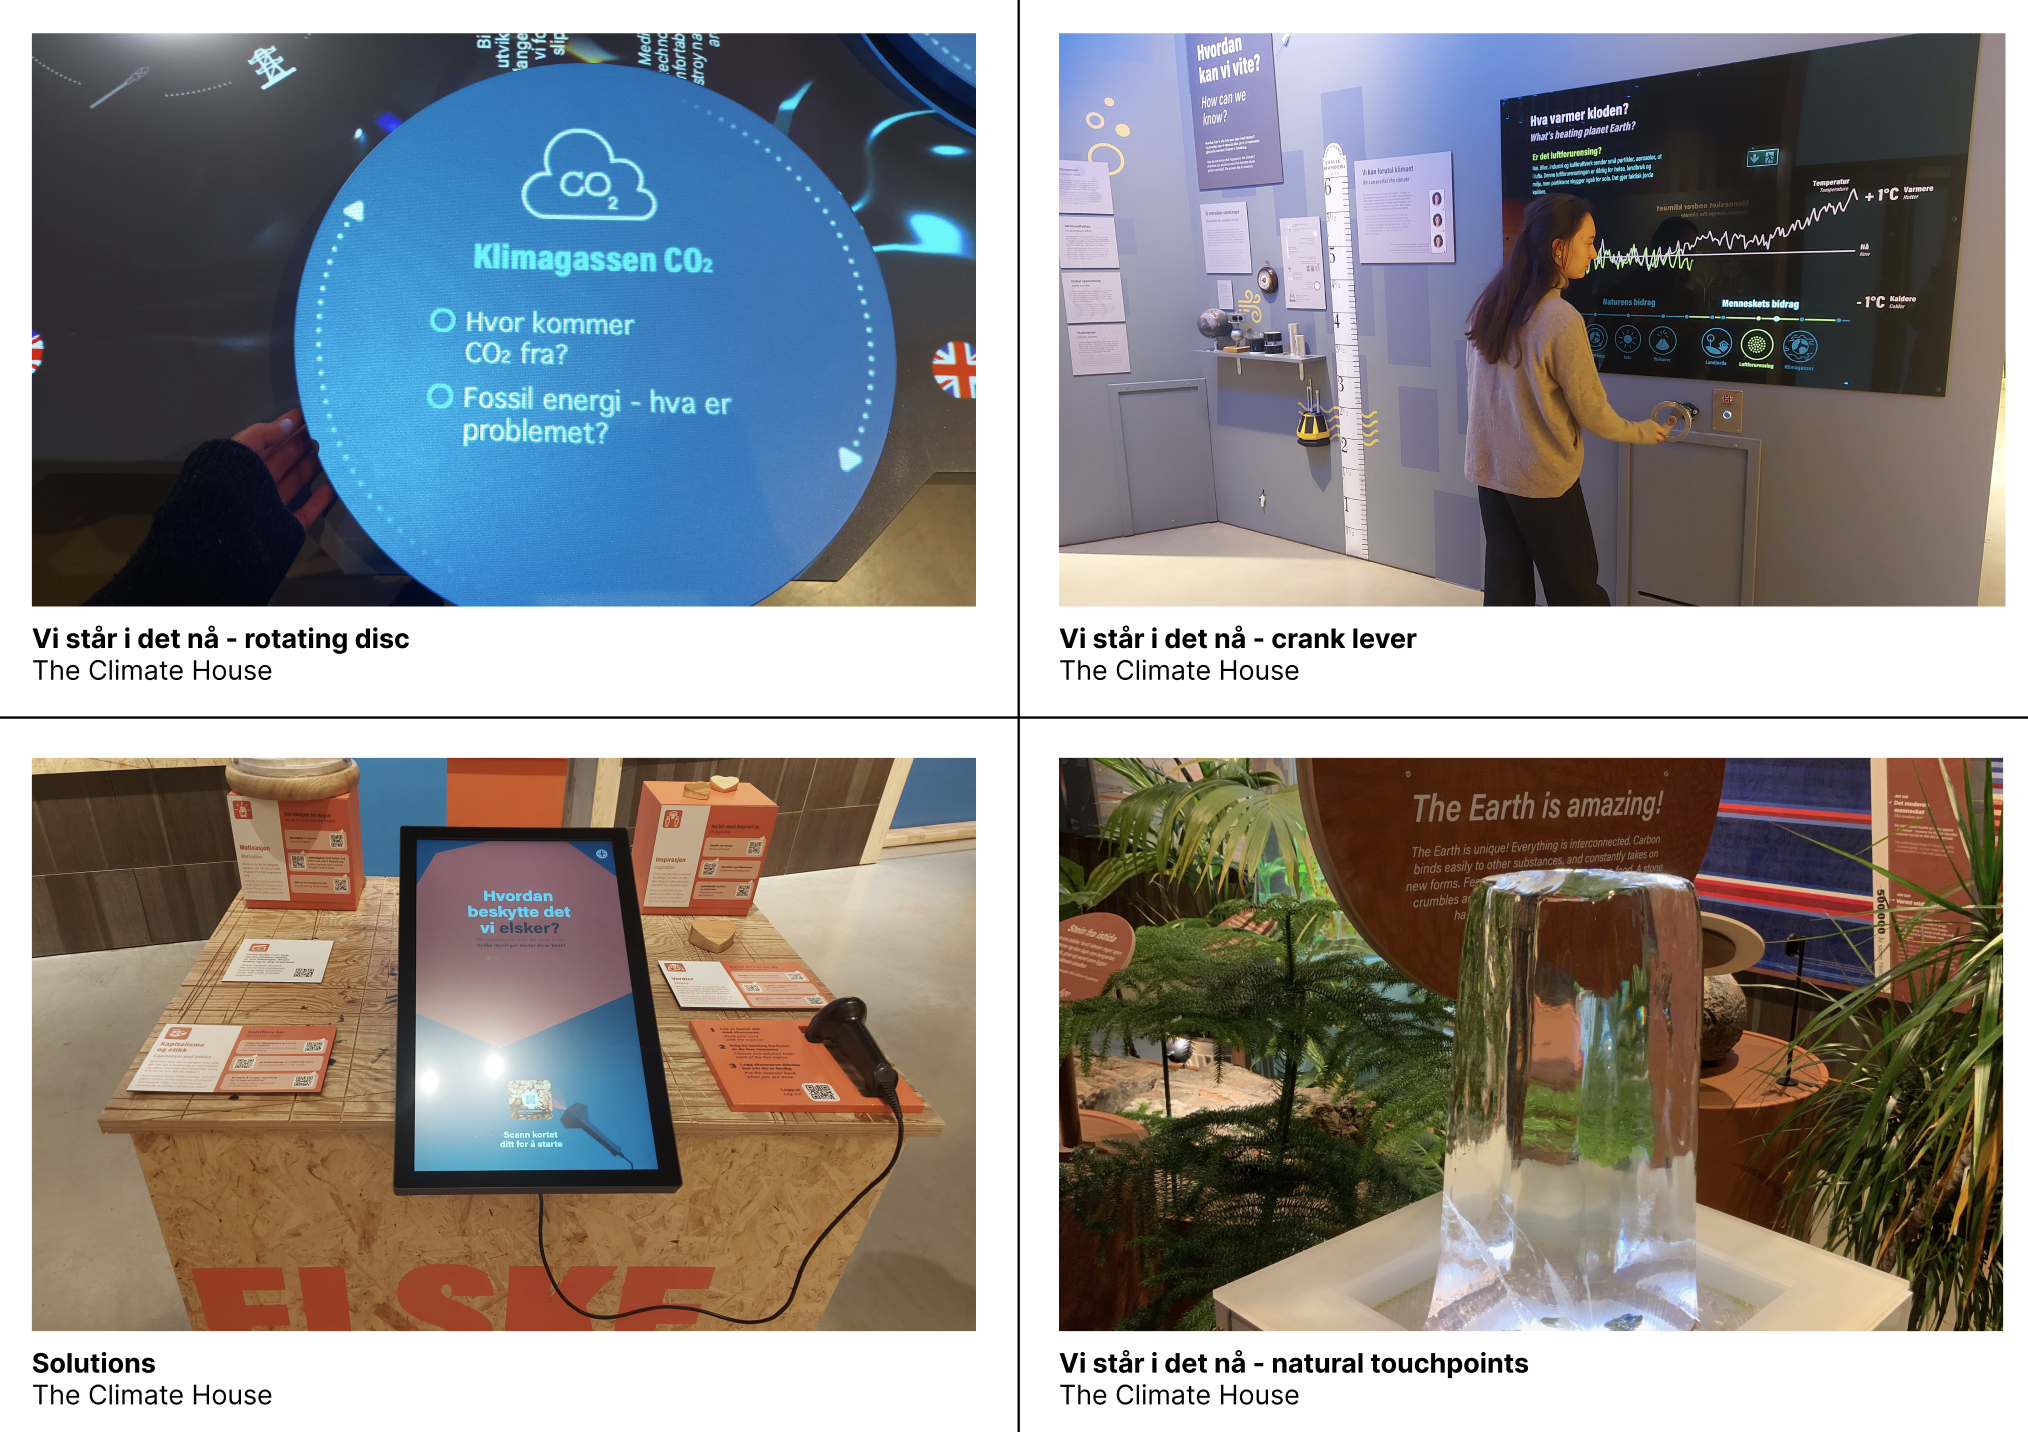
\includegraphics[width=13cm]{pictures/dataset/klimahuset.png}
\centering 
\end{figure}

\begin{figure}[H]
\includegraphics[width=13cm]{pictures/dataset/Qi.pdf}
\centering 
\end{figure}

\begin{figure}[H]
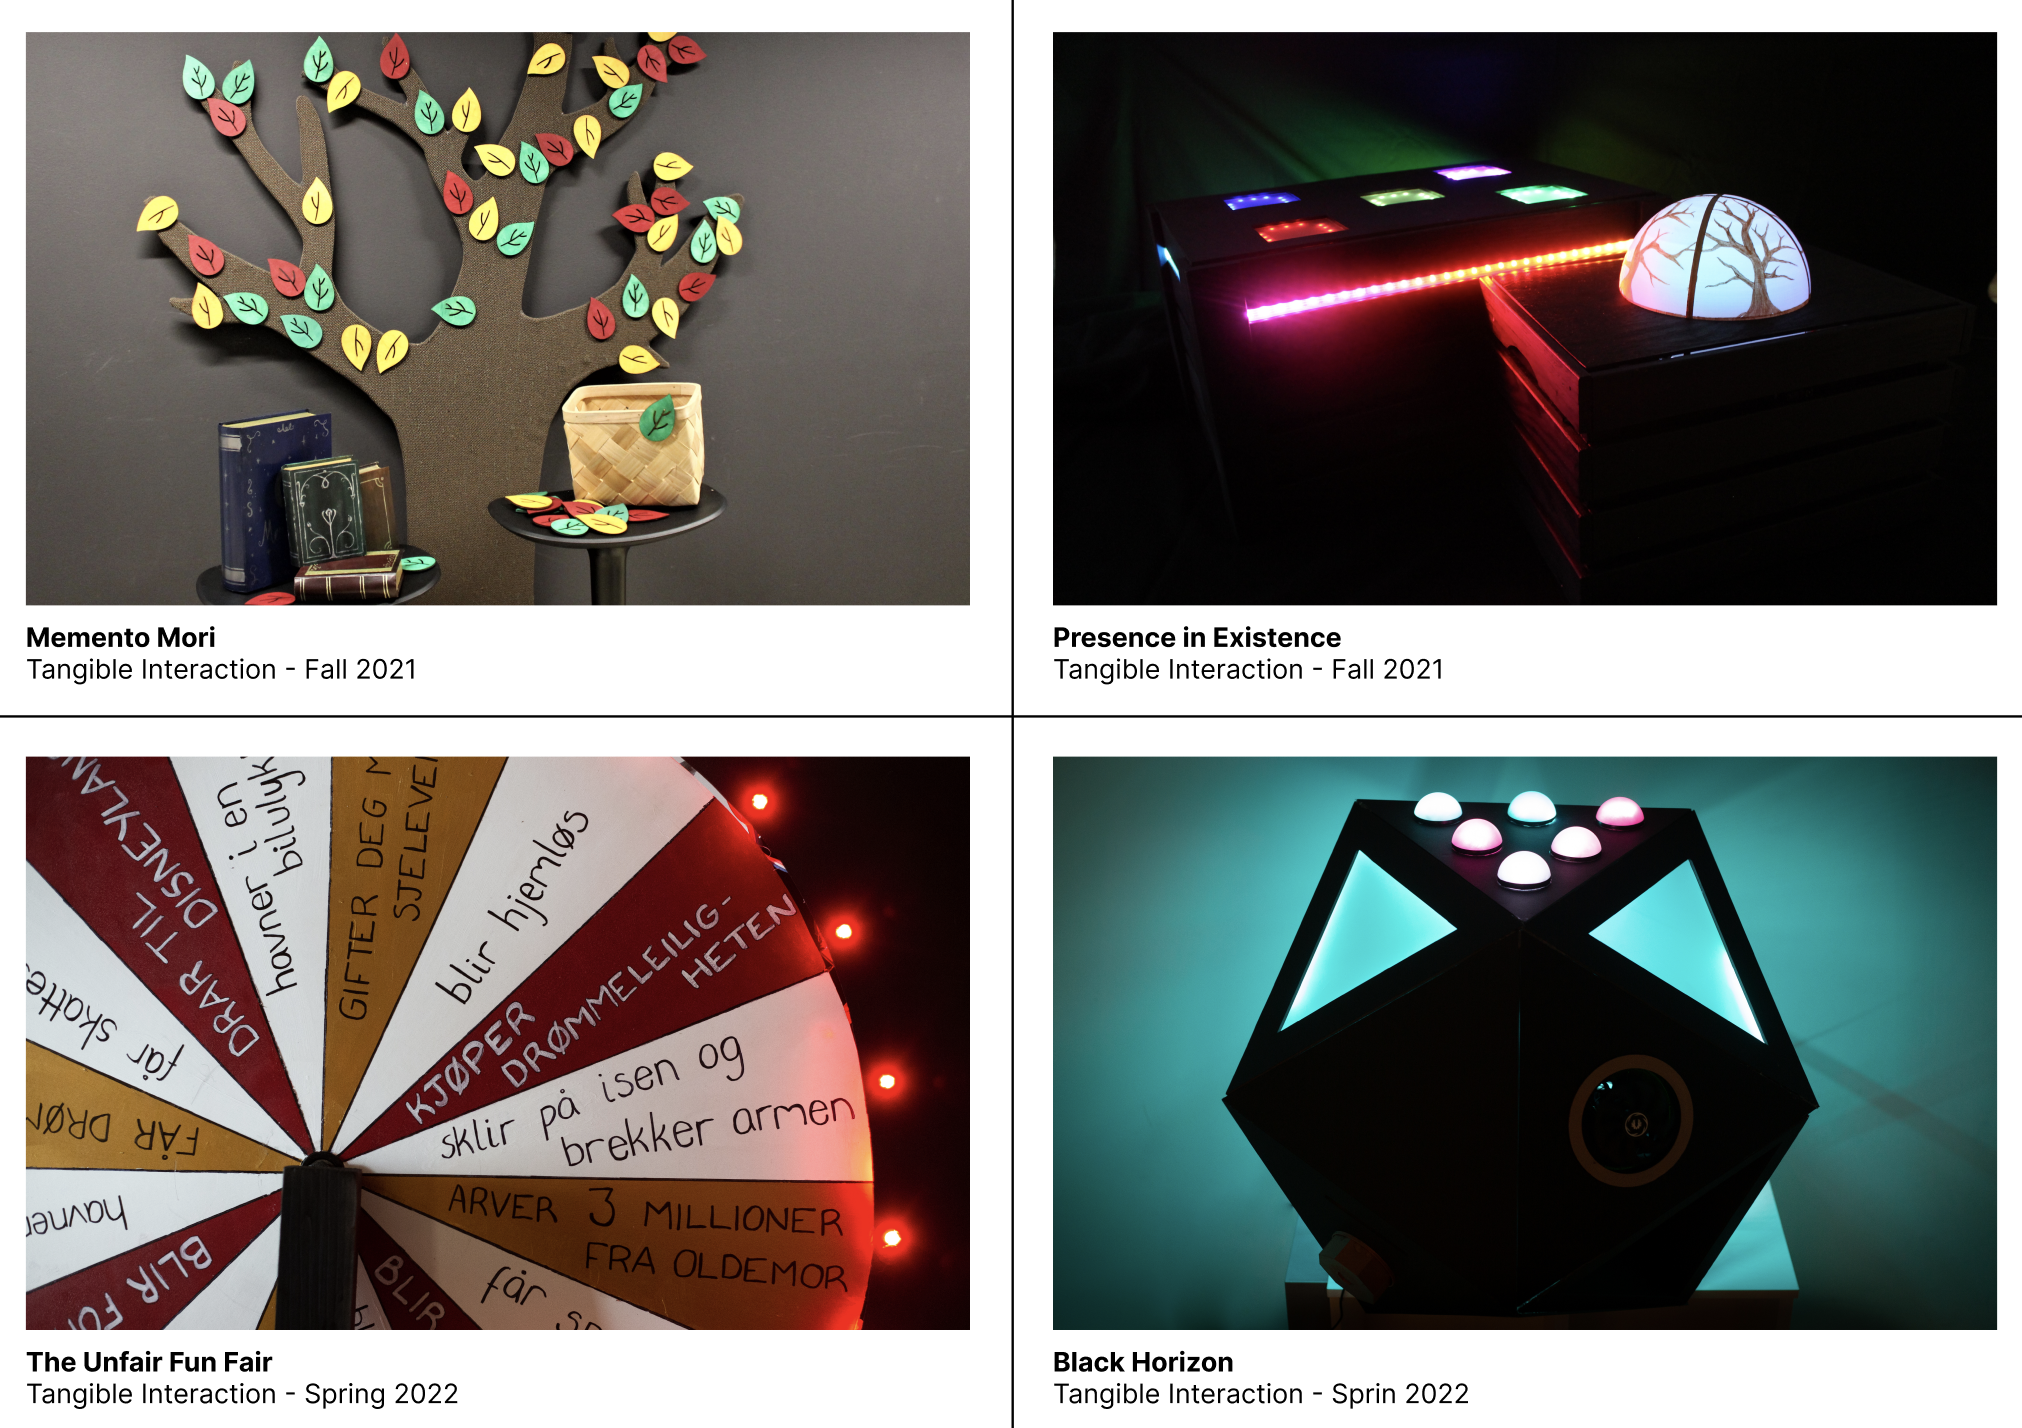
\includegraphics[width=13cm]{pictures/dataset/tangible.png}
\centering 
\end{figure}

\begin{figure}[H]
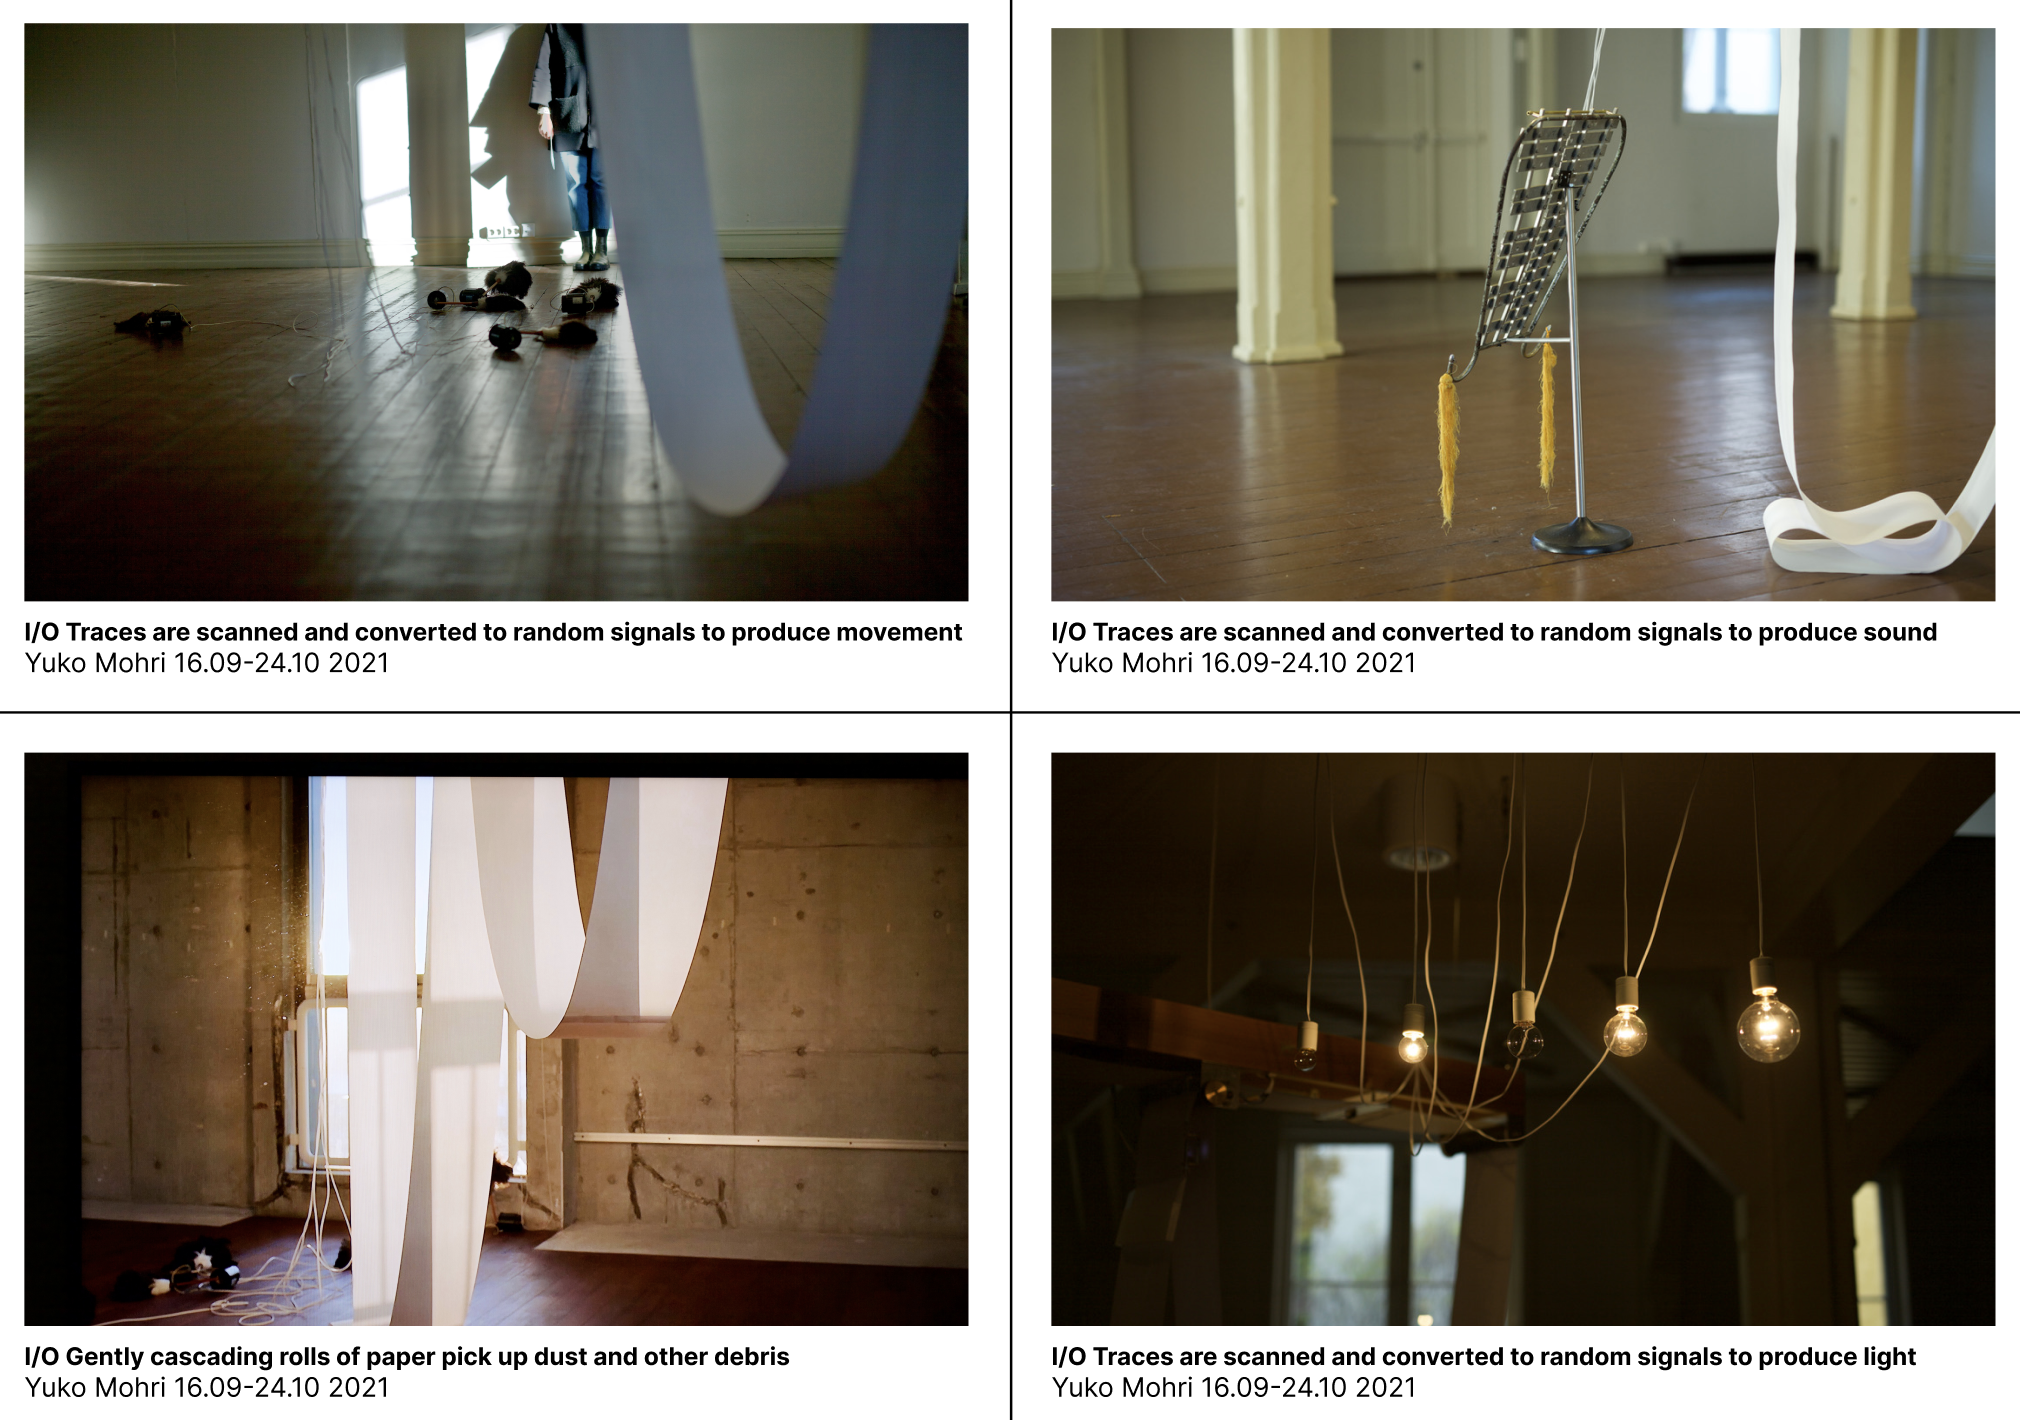
\includegraphics[width=13cm]{pictures/dataset/yuko_mohri.png}
\centering 
\end{figure}

\section{Consent forms}

\begin{figure}[H]
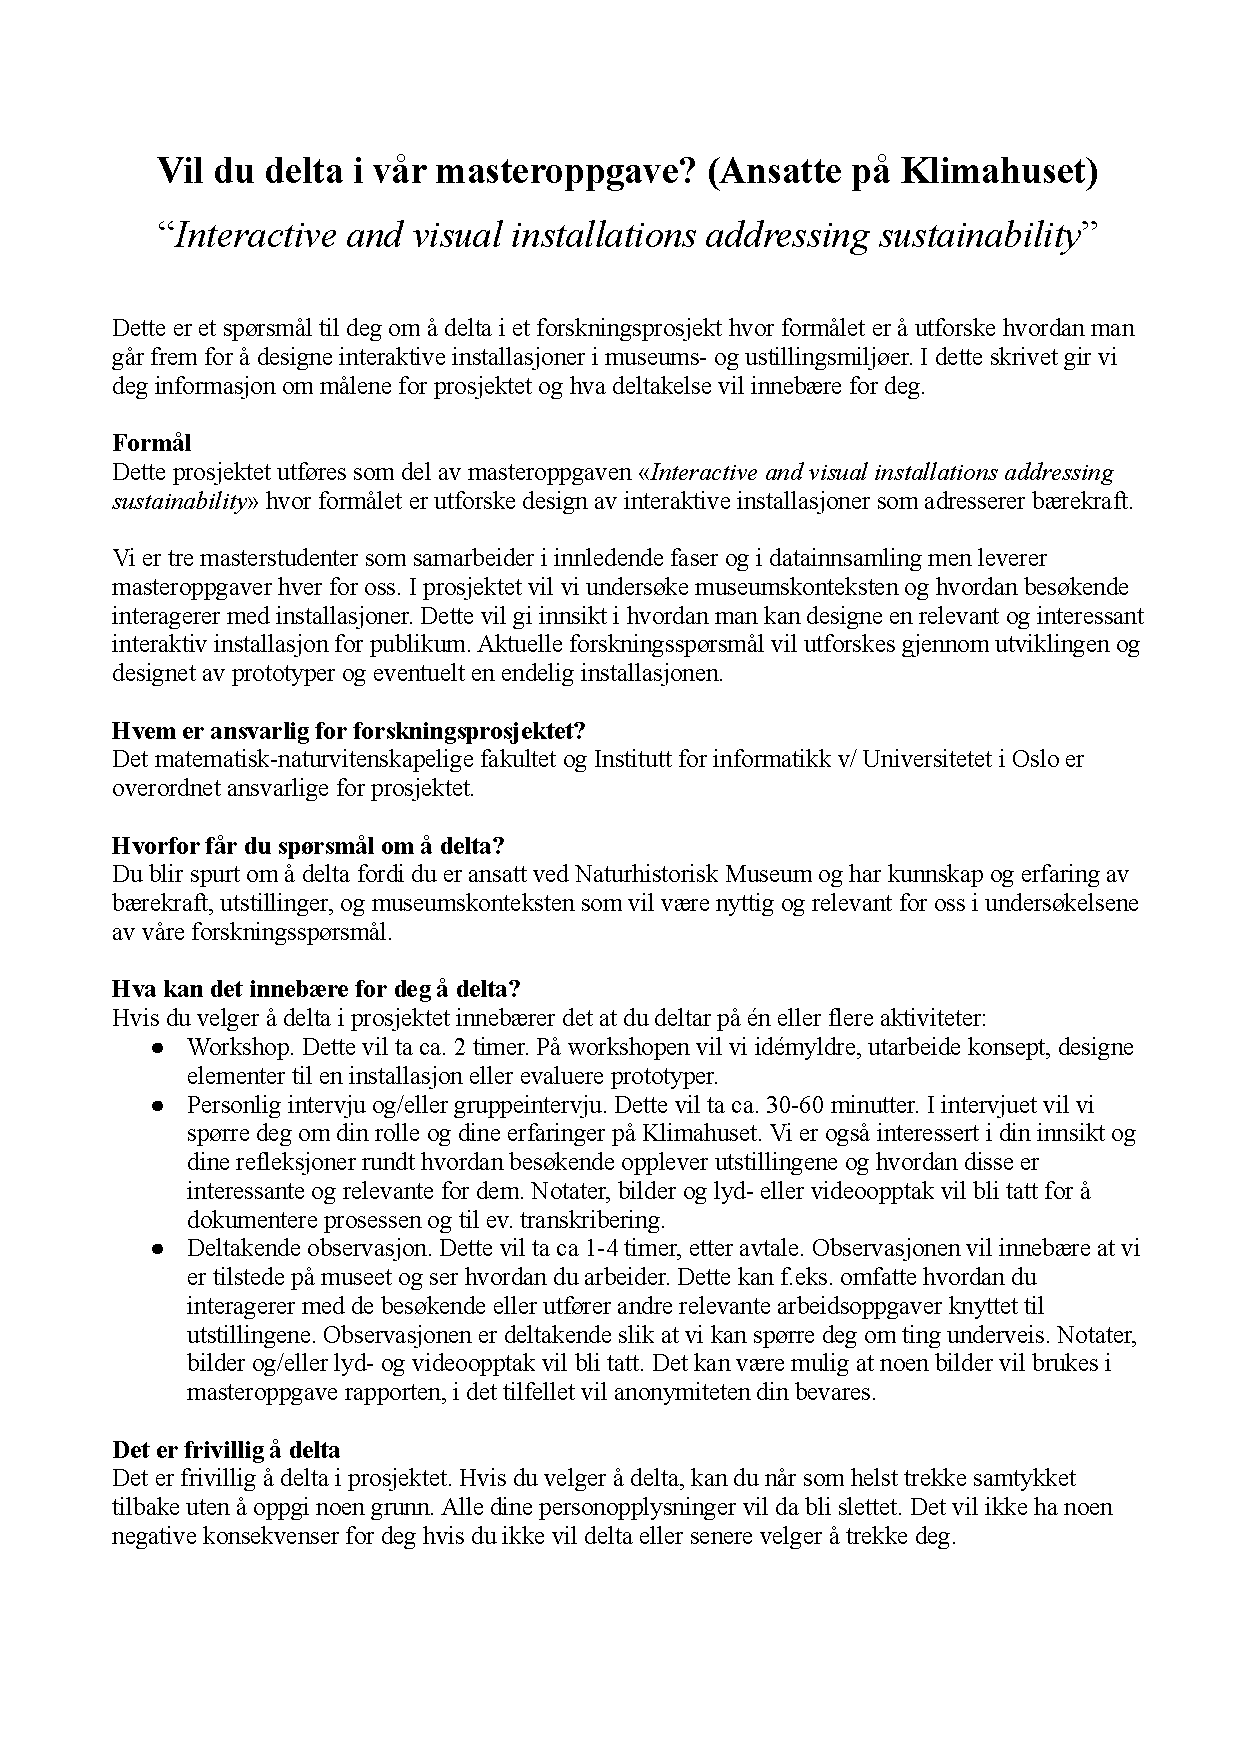
\includegraphics[width=12.5cm]{pictures/appendix/Samtykkeskjema_klimahuset.pdf}
\caption{Consent form for employees at Klimahuset}
\end{figure}

\begin{figure}[H]
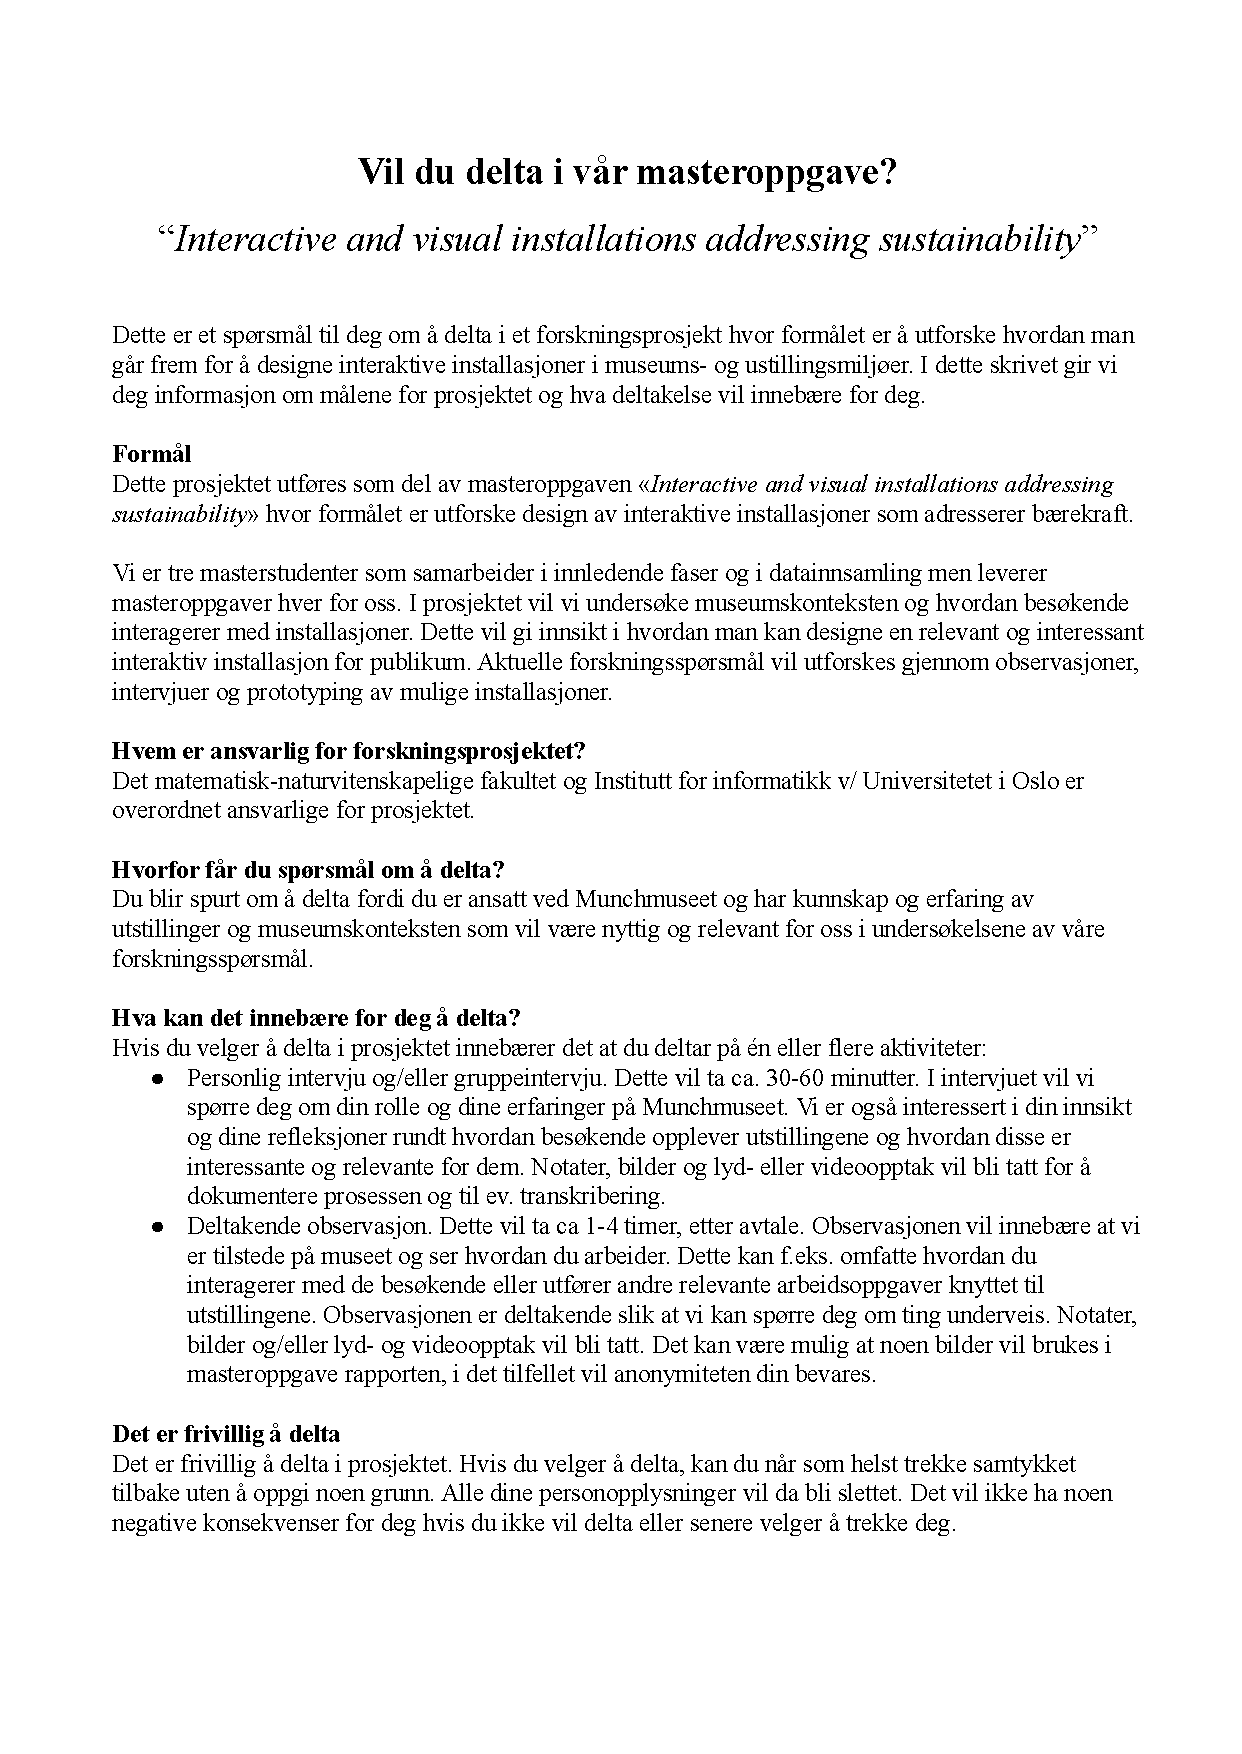
\includegraphics[width=12.5cm]{pictures/appendix/Samtykkeskjema Munch.docx.pdf}
\caption{Consent form for employees at Klimahuset}
\end{figure}



\end{document}